%% English-only manuscript. Chinese paragraph translations are omitted.
%% Compile from this folder with MiKTeX:
%%   $env:TEXINPUTS = ".;..;"; xelatex main.tex; bibtex main; xelatex main.tex; xelatex main.tex
%% 
%% Copyright 2019-2024 Elsevier Ltd
%% 
%% Version 2.4
%% 
%% This file is part of the 'CAS Bundle'.
%% --------------------------------------
%% 
%% It may be distributed under the conditions of the LaTeX Project Public
%% License, either version 1.2 of this license or (at your option) any
%% later version.  The latest version of this license is in
%%    http://www.latex-project.org/lppl.txt
%% and version 1.2 or later is part of all distributions of LaTeX
%% version 1999/12/01 or later.
%% 
%% The list of all files belonging to the 'CAS Bundle' is
%% given in the file `manifest.txt'.
%% 
%% Template article for cas-dc documentclass for 
%% double column output.

\PassOptionsToPackage{no-math}{fontspec}
\documentclass[a4paper,fleqn]{cas-dc}
\graphicspath{{../}}

% Allow continuous Type1 scaling (STIX/.fd discrete sizes → ≤0.5pt substitution warning)
\usepackage{anyfontsize}

%\usepackage[authoryear,longnamesfirst]{natbib}
%\usepackage[authoryear]{natbib}
\usepackage[numbers]{natbib}
\usepackage{array}

%%%Author definitions
\def\tsc#1{\csdef{#1}{\textsc{\lowercase{#1}}\xspace}}
\tsc{WGM}
\tsc{QE}
\tsc{EP}
\tsc{PMS}
\tsc{BEC}
\tsc{DE}
%%%Mine

\DeclareMathOperator*{\argmax}{arg\,max}
\DeclareMathOperator*{\argmin}{arg\,min}
\usepackage[ruled,vlined]{algorithm2e}
\DontPrintSemicolon
\SetAlFnt{\footnotesize}
\SetAlCapFnt{\footnotesize}
\SetAlCapNameFnt{\footnotesize\bfseries}
\SetAlgoSkip{smallskip}
\SetInd{0.4em}{0.7em}
\SetCommentSty{textit}
\hypersetup{
  colorlinks=False,
  citecolor=Violet,
  linkcolor=Red,
  urlcolor=Blue}
% Make bibliography DOI identifiers resolve directly to the publisher landing page.
\providecommand{\doi}[1]{\href{https://doi.org/#1}{\nolinkurl{doi: #1}}}

\usepackage{tabularx}
\usepackage{multirow}
\usepackage{makecell}
\usepackage{booktabs}
\usepackage{subcaption}
% Figure/table captions: small Times New Roman, bold "Figure N:" label, colon separator.
\captionsetup{font={small,rm},labelfont={bf,rm},labelsep=colon}
\usepackage{xcolor}
\usepackage{soul}
\usepackage{amsthm}
\usepackage{amsmath}
\usepackage{placeins}
\usepackage{fontspec}
% Body text and captions in Times New Roman.
% Mathematical symbols keep the class math font.
\IfFontExistsTF{Times New Roman}
  {\setmainfont{Times New Roman}
   \setmonofont{Times New Roman}}
  {\setmainfont{lmroman10-regular.otf}
   \setmonofont{lmmono10-regular.otf}}
\IfFontExistsTF{Arial}
  {\setsansfont{Arial}}
  {\IfFontExistsTF{Helvetica}
    {\setsansfont{Helvetica}}
    {\setsansfont{lmsans10-regular.otf}}}
% Tables (body and caption) stay in Times New Roman for numeric alignment.
\IfFontExistsTF{Times New Roman}
  {\newfontfamily\tablefont{Times New Roman}}
  {\newcommand{\tablefont}{\rmfamily}}
% cas-common hardcodes \sffamily in figure/table floats and captions; remap
% \sffamily to Times New Roman inside those environments.
\newcommand{\tablestyle}{\let\sffamily\tablefont\tablefont}
\AddToHook{env/table/begin}{\tablestyle}
\AddToHook{env/table*/begin}{\tablestyle}
\AddToHook{env/tabular/begin}{\tablefont}
\AddToHook{env/tabular*/begin}{\tablefont}
\AddToHook{env/tabularx/begin}{\tablefont}
\newcommand{\figurestyle}{\let\sffamily\tablefont\tablefont}
\AddToHook{env/figure/begin}{\figurestyle}
\AddToHook{env/figure*/begin}{\figurestyle}
% Use the final shipped-page count, including deferred appendix floats.
\AtBeginDocument{\renewcommand{\lastpage}{\PreviousTotalPages}}
% Page headers/footers: cas-common hardcodes \sffamily; force Times New Roman.
% Top-align float pages (avoid vertically centred orphan appendix figures).
\makeatletter
\setlength{\@fptop}{0pt}
\setlength{\@fpsep}{8pt plus 1fil}
\setlength{\@fpbot}{0pt plus 1fil}
\makeatother
\ExplSyntaxOn
\cs_set:Npn \__cas_head:
  {
    \parbox{\textwidth}{ \rmfamily\small\centering \__short_title: }
  }
\cs_set:Npn \__cas_foot:
  {
    \parbox[t]{\textwidth}
      {
        \rule{\textwidth}{.2pt}\\
        \rmfamily\small
        \__first_footerline:
        \hfill Page~\thepage {}~of~ \PreviousTotalPages
      }
  }
\cs_set:Npn \__first_footerline:
  {
    \group_begin:
    \small\rmfamily
    \ifnum\theblind>0\relax
    \else
      \__short_authors: :~
    \fi
    { \itshape Preprint~ submitted ~to ~Elsevier }
    \group_end:
  }
\AddToHook{begindocument/end}
  {
    \pagestyle{cas}
  }
\ExplSyntaxOff
\newcommand{\uprep}{$R_{\mathrm{up}}^{\mathrm{rep}}$}
\newcommand{\upwho}{$R_{\mathrm{up}}^{\mathrm{who}}$}
\newcommand{\onwho}{$R_{\mathrm{on}}^{\mathrm{who}}$}
\newcommand{\na}{---}
\renewcommand{\labelitemi}{\ensuremath{\bullet}}
\newtheorem{assumption}{Assumption}[section]
\usepackage[switch]{lineno}

% The class prints "orcid(s):" even when no ORCID is given.
\ExplSyntaxOn
\RenewDocumentCommand \printorcid { }
  {
    \seq_if_empty:NF \g_stm_orcid_seq
      {
        \group_begin:
          \tex_let:D \thefootnote \relax \footnotetext
            {
              \raggedright
              \textsc{orcid}(s):\c_space_token
              \seq_use:Nn \g_stm_orcid_seq { ;~ }
            }
        \group_end:
      }
  }
\ExplSyntaxOff

%%%%%%

\begin{document}
%% Bibliography order by work relevance: [1] PDFormer, [2] STGNPP, then factory GNN/LSTM predictors, detection reviews, DT/diagnosis, HRC/multimodal.
\emergencystretch 3em %%%exceed margin
\let\WriteBookmarks\relax
\def\floatpagepagefraction{1}
\def\textpagefraction{.001}
\shorttitle{Process-informed heterogeneous graph learning with delayed propagation for dynamic bottleneck prediction in manufacturing}
\shortauthors{Yuxiao Tian et al.}

\title [mode = title]{Process-informed heterogeneous graph learning with delayed propagation for dynamic bottleneck prediction in manufacturing}

\author[1]{Yuxiao Tian}[]
\credit{Conceptualization, Methodology, Data curation, Original draft}
\author[1]{Xiao Li}[]
\cormark[1]
\credit{Conceptualization, Supervision, Review \& editing}
\author[1]{Jintao Xue}[]
\credit{Conceptualization, Methodology, Data curation, Review \& editing}
\author[1]{Wantong Xu}[]
\credit{Investigation, Validation}
\affiliation[1]{organization={CI3 Lab, Department of Civil Engineering, The University of Hong Kong},
                city={Hong Kong SAR},
                }

\cortext[cor1]{Corresponding author: CI3 Lab, Department of Civil Engineering, Faculty of Engineering, The University of Hong Kong, Pokfulam, Hong Kong, China.}

\begin{abstract}
Dynamic bottleneck prediction is essential in multi-entity production systems.
Existing studies face limitations in observation scope and bottleneck supervision.
They mainly rely on single-entity data from workstations, with limited representation of multiple entities including workers, materials, buffers, and logistics and the relations among them.
This narrow observation scope leads to incomplete factory-graph modelling, making it difficult to capture delayed propagation across resources and thereby reducing prediction accuracy.
In addition, constructing reliable bottleneck supervision is difficult: bottleneck events are scarce, while simple threshold-based labels may mistake short-term changes for lasting bottlenecks and provide little information about their causes.
To address these limitations, we propose the \textbf{Process-Informed Heterogeneous-Graph Spatiotemporal Transformer with a Propagation-Delay-Aware Module (PHGST-PD)}.
Firstly, to broaden the observation scope, PHGST-PD combines a heterogeneous process--logistics graph with a propagation-delay-aware module guided by recurrent operating patterns, linking earlier resource states to operating changes that emerge elsewhere after a propagation delay.
Secondly, to improve bottleneck supervision, process-informed supervision generates labels for sustained bottlenecks and their causes, while clustering identifies repeated operating patterns.
In addition, the model extends bottleneck prediction beyond simple temporal estimates to provide a more comprehensive bottleneck description.
It jointly outputs bottleneck station, onset, duration, process cause, and remaining order time.
Experiments in the evaluated simulation setting demonstrate higher event-prediction accuracy than the compared baselines and detailed bottleneck forecasts, while ablation studies support the contributions of heterogeneous resource information, process-informed supervision, and the propagation-delay-aware module.
These results highlight the potential of PHGST-PD to provide advance warning of bottlenecks and inform timely resource interventions in multi-entity production systems.

\end{abstract}

\begin{keywords}
Multi-entity production systems \sep
Dynamic Bottleneck Prediction \sep
Process-aware weak supervision \sep
Spatiotemporal Transformer \sep
Propagation Delay
\end{keywords}

\begin{NoHyper}
\maketitle
\end{NoHyper}

%% ========================================================================
\section{Introduction} \label{sec:intro}
%% ========================================================================

A production bottleneck is the resource or process that limits system throughput at a given time~\cite{subramaniyan2023throughput,tang2024comprehensive}. Its identity and location are dynamic: changes in resource availability, material supply, work-in-process, and operating conditions can cause the bottleneck to migrate during production~\cite{lai2021data}. Timely and accurate prediction of these changes is therefore important for production management: advance warning can inform resource allocation and production scheduling.

Existing bottleneck-prediction studies face two limitations. First, existing studies mainly model workstation data. Time-series and recurrent methods forecast active periods, blockage, starvation, or bottleneck scores from workstation-centred observations~\cite{li2011throughput,subramaniyan2018data,lai2018twolayer,liu2023lstmdam}; graph-based methods further introduce task or material-flow relations~\cite{lai2023bstan,yin2025btgcn,ma2023tusb,cen2025dstnn,wu2025knowledge}. Nevertheless, workers, material availability, buffers, and transport resources are rarely represented together, even though their interactions can determine where and when a bottleneck appears. This narrow observation scope leaves the factory graph incomplete and makes delayed cross-resource propagation difficult to capture: an operating change may pass through transport and buffering before emerging as blockage or starvation at a downstream station, so the resource where the operating change originates may differ from the resource that later constrains throughput~\cite{gu2015passive,zhang2022vulnerability}. Recurrent transmission and local graph aggregation can capture temporal or neighbourhood dependence~\cite{liu2023lstmdam,yin2025btgcn}, but do not explicitly align an earlier cross-resource pattern with its delayed consequence.

Second, bottleneck supervision is difficult to construct. Bottleneck events are scarce in normal operation, and deliberately inducing failures, worker absence, material shortages, or logistics interruption to obtain training data is not feasible during real factory production. Conventional scalar scores and turning-point indicators derived from utilization, blockage, or starvation~\cite{subramaniyan2023throughput,lai2021data,su2022dynamic} can support retrospective analysis. However, when such indicators are used alone to construct prediction targets, they reduce a changing production process to a narrow decision criterion and may ignore the combined evidence of queues, resource availability, material shortages, and logistics conditions. Without this process context, the resulting labels may mistake short-term changes for lasting bottlenecks and assign similar labels to events with different operational causes. Such ambiguous targets can limit prediction accuracy and make the causes of predicted events difficult to interpret. These limitations motivate a unified approach to heterogeneous observation, process-informed supervision, and delay-aware prediction.

To address these limitations, we propose the \textbf{Process-Informed Heterogeneous-Graph Spatiotemporal Transformer with a Propagation-Delay-Aware Module (PHGST-PD)}. First, to broaden the observation scope and capture delayed interactions, PHGST-PD combines a heterogeneous process--logistics graph with a propagation-delay-aware module guided by recurrent operating patterns. An open-workspace factory model developed for NVIDIA Isaac Sim provides traceable trajectories of workstations, workers, material supply, buffers, and transport resources under configurable operating conditions~\cite{lu2020digital,isaacsim2026,xue2026safe}. These observations are organized as a heterogeneous process--logistics graph: workstations and handling resources are represented as interacting entities, while material shortage, buffer occupancy, labour availability, and transport delay provide resource-specific operational context. This representation brings production and logistics observations into a shared graph, allowing the predictor to account for interactions beyond workstation states alone. The propagation-delay-aware module matches recent resource trajectories to fixed temporal-pattern prototypes and conditions cross-resource attention on the resulting pattern context. Earlier resource states can therefore contribute to the prediction of bottlenecks that emerge elsewhere after transport or buffering delay. Second, to improve bottleneck supervision, process-informed supervision combines queue, blockage, starvation, availability, shortage, and logistics evidence with persistence requirements. This supervision distinguishes sustained bottleneck events from short-term fluctuations and assigns observable process-cause targets, connecting supervision to traceable production evidence. Clustering summarizes training-only short temporal patches as recurrent operating-pattern prototypes, providing the pattern context used by the propagation-delay-aware module. Together, these components provide bottleneck-event and process-cause supervision.

In addition, PHGST-PD extends bottleneck prediction beyond simple temporal estimates to provide a more comprehensive bottleneck description. The model jointly outputs bottleneck station, onset, duration, observable process cause, and remaining order time, providing a minute-level report to support advance warning and timely resource intervention. In the evaluated simulation setting, PHGST-PD achieves higher event-prediction accuracy than the compared baselines and generates detailed forecasts. Ablation studies further support the contributions of heterogeneous resource information, process-informed supervision, and the propagation-delay-aware module. These results highlight the potential of PHGST-PD to provide advance warning of emerging bottlenecks and inform timely resource interventions in multi-entity production systems.

The contributions of this work are summarized as follows.

(1) We extend dynamic bottleneck prediction from workstation-centred observations to heterogeneous multi-entity factory data. Workstations, workers, material-supply states, buffers, and transport resources are jointly represented with their process and logistics relations, enabling the model to capture bottlenecks arising from production, labour, material, and handling interactions rather than from workstation states alone.

(2) We develop \emph{process-informed supervision and temporal pattern clustering} for bottleneck data whose events are scarce and weakly separable from normal fluctuations. Resource-specific rules and persistence constraints construct operationally meaningful event and process-cause targets, deterministic cause-aligned regime identifiers provide structured context, and training-only clustering summarizes short temporal patches as recurrent operating-pattern prototypes. This design provides reliable supervision to improve bottleneck-identification accuracy.

(3) We propose a \emph{propagation-delay-aware module guided by recurrent operating patterns}. It matches recent resource trajectories to fixed temporal-pattern prototypes and injects the resulting pattern context into cross-resource geographic attention, allowing the model to associate an upstream precursor with a downstream bottleneck that appears after transport or buffering delay.

The remainder of this paper is organized as follows. Section~\ref{sec:review} reviews bottleneck detection and prediction methods and spatiotemporal graph forecasting. Section~\ref{sec:problem} formulates the station-level dynamic bottleneck prediction problem. Section~\ref{sec:method} presents the factory-model data pipeline and PHGST-PD architecture. Section~\ref{sec:exp} reports the experimental setup and results.

%% ========================================================================
\section{Literature review} \label{sec:review}
%% ========================================================================

\subsection{Dynamic bottleneck prediction concepts and task scope}

A throughput bottleneck is a resource or process that constrains the overall output of a manufacturing system. Skoogh et al.~\cite{subramaniyan2023throughput} show that bottleneck-identification methods differ in both the information they use and how they are operationalized; the appropriate choice depends on the system and on the available data. High utilization, a failure, or a queue at an individual resource can provide useful evidence, but its effect on system throughput must be interpreted together with the other resources and process relations.

The dynamic nature of a bottleneck depends on the observation time scale. A bottleneck that dominates over a long period may migrate when processing conditions, resource availability, or material supply changes. Lai et al.~\cite{lai2021data} addressed shifting bottlenecks in complex manufacturing systems by combining production data with factory-physics knowledge and extending the turning-point method to non-serial configurations. Dynamic bottleneck research therefore concerns both the constrained location and the trajectory of that constraint as production evolves.

Detection identifies a constraint from a process that has already occurred or is currently occurring, whereas prediction uses historical and current observations to infer a future state. Subramaniyan et al.~\cite{subramaniyan2021ai} classify artificial-intelligence-supported throughput bottleneck analysis into identification, diagnosis, prediction, and prescription. The classification separates future prediction from detection and decision support: updating a detection result in real time does not by itself constitute advance prediction.

Existing prediction studies follow three main approaches: extrapolating bottleneck indicators, adapting to changing production conditions, and explicitly modelling production relations. Subramaniyan et al.~\cite{subramaniyan2018data} combined ARIMA with machine active-period analysis to predict throughput bottlenecks, while Huang et al.~\cite{huang2019proactive} used future bottleneck predictions to support proactive task dispatching. Liu et al.~\cite{liu2023lstmdam} constructed bottleneck indicators from station supply--demand relations, learned temporal dependencies with a dual-attention LSTM, and updated the model through concept-drift detection and transfer learning. Ma et al.~\cite{ma2023tusb} jointly modelled spatial and temporal information for high-variety shops with complex routings, and Lai et al.~\cite{lai2023bstan} predicted blockage and starvation from station relations before inferring future bottlenecks. These studies extend prediction from single-indicator extrapolation to production relations and adaptation to changing operating conditions.

For production warning, a prediction must have an explicit temporal meaning so that it can support scheduling, resource allocation, and process intervention. Existing event-prediction studies commonly consider whether a constrained event will occur, where it will occur, when it will start, and how long it will last. For an event that is already active, its remaining duration can also be estimated. Dynamic bottleneck prediction can therefore organize continuous indicators or state decisions into advance-warning information with explicit temporal attributes.

\subsection{Bottleneck indicators and input representation}

Constructing a state representation from production records requires explicit definitions of the observed resources, time range, and indicator semantics. Queue length, waiting time, activity ratio, and blockage or starvation time describe different aspects of resource operation and can form a multi-dimensional observation. Skoogh et al.~\cite{subramaniyan2023throughput} group bottleneck-detection information into queue states, process states, and combinations of the two, representing product accumulation and waiting, resource activity, and constrained operating conditions. Subramaniyan et al.~\cite{subramaniyan2016realtime} computed average active periods from machine states and their timestamps in real-time MES data to identify production bottlenecks. Compared with a point-wise state or a window-level activity ratio, a continuous active period preserves persistence information, showing that indicator design must also reflect the temporal organization of production changes.

The resulting multi-dimensional indicators can be processed in two complementary ways: process knowledge can define state rules, or data similarity can reveal operating regimes. The first approach combines resource activity, material supply, and neighbouring-process relations to interpret blockage, starvation, or other production conditions. Lai et al.~\cite{lai2021data} combined blockage and starvation information with production-structure knowledge for complex manufacturing systems, while Liu et al.~\cite{liu2023lstmdam} used station supply--demand relations to construct predictive indicators. The second approach clusters machine indicator sequences or multi-dimensional window observations according to similarity. Subramaniyan et al.~\cite{subramaniyan2020clustering} generated bottleneck-indicator time series from event logs and used dynamic-time-warping distance with agglomerative hierarchical clustering to group machines with similar production dynamics. For multi-dimensional window samples, K-means can also summarize similar operating conditions, although its result depends on the feature representation and similarity measure~\cite{jain2010clustering}. Process rules produce interpretable state judgements, whereas clustering produces groups of similar samples; the two can be combined. A cluster is therefore a recurrent operating pattern rather than a bottleneck label, and its production meaning must be interpreted from within-cluster features and domain knowledge before being mapped to state or cause categories.

After indicators and states or regimes have been defined, model inputs generally contain both continuous and categorical variables. Queue length, waiting time, and activity ratio preserve numerical changes in resource constraints, while resource type and rule- or pattern-derived state labels provide categorical information. Because these variables have different representation forms, they are often encoded separately before being mapped into a common vector space. Temporal Fusion Transformer (TFT) embeds categorical variables, linearly projects continuous variables, and uses a variable-selection network to combine them~\cite{lim2021tft}. Indicators quantify the observed resource conditions. State rules and regime analysis add process interpretations or identify similar operating patterns, while input encoding converts these heterogeneous observations into model representations.

\subsection{Delayed cross-resource effects in production systems}\label{sec:manufacturing-delay}

Manufacturing-system studies show that finite buffers can delay the transmission of disruption effects between resources. Finite buffers can temporarily decouple neighbouring stations: an upstream interruption need not starve a downstream machine until the available work-in-process is consumed, while a downstream interruption need not block an upstream machine until the intervening storage fills. Gu et al.~\cite{gu2013hidden} analysed these buffering effects through maintenance opportunity windows in discrete and complex production lines, with simulations and real automotive-assembly-plant cases. Gu et al.~\cite{gu2015passive} further predicted failure-induced starvation or blockage intervals on bottleneck machines when other machines fail upstream or downstream, and validated their algorithm using simulations and an automotive assembly plant. These studies establish an operational reason to consider both the originating disruption and its later effect on a different resource.

Zhang et al.~\cite{zhang2022vulnerability} made the delay explicit in a finite-buffer smartphone-assembly model by defining \emph{Bottleneck Time Delay} as the interval from a disruption to production stoppage at the bottleneck station. Their analysis relates this interval to the disruption location and the intervening buffer occupancy, and distinguishes it from the delay before the end-of-line station stops. The study provides analytical and numerical evidence through a smartphone-production digital-twin evaluation tool. Taken together, this literature supports delayed transmission of disruption effects, rather than the assumption that every local disruption immediately changes system throughput. It also distinguishes such transmission from bottleneck migration: a bottleneck can be affected by a remote disruption without its location changing. For prediction, this motivates using earlier observations of related resources together with the target resource's recent state. The remaining modelling question is how to exploit that lagged evidence in a heterogeneous, multi-entity event predictor, rather than whether manufacturing propagation delays exist.

\subsection{Graph-based spatiotemporal modelling and event prediction}

Manufacturing resources form networks through process precedence, material transfer, and shared tasks. Representing resources, workstations, or tasks as nodes and production relations as edges allows a model to use related resources when analysing an individual object. Graph neural networks learn node representations through neighbourhood propagation and aggregation~\cite{wu2021gnn}. GCN aggregates neighbourhood information according to a normalized graph structure~\cite{kipf2017gcn}, whereas GAT learns the contribution weight of each neighbour from node features~\cite{velickovic2018gat}. For dynamic production, these spatial mechanisms must be combined with temporal modelling to describe the evolution of resource states and their interactions.

Traffic forecasting has developed a broad family of multi-node spatiotemporal models, which provides a useful methodological reference for organizing spatial relations and historical information in manufacturing resource networks. DCRNN embeds diffusion convolution in a recurrent structure and combines spatial propagation with sequence modelling on directed graphs~\cite{li2018dcrnn}. STGCN extracts spatiotemporal features through graph convolution and gated temporal convolution~\cite{yu2018stgcn}. Graph WaveNet learns an adaptive adjacency relation from node embeddings and processes historical sequences with dilated causal temporal convolutions~\cite{wu2019graphwavenet}, while STSGCN constructs local spatiotemporal graphs connecting adjacent time steps to aggregate spatial and temporal neighbours jointly~\cite{song2020stsgcn}. These methods organize dynamic dependence through diffusion and recurrence, graph and temporal convolution, adaptive relation learning, or joint spatiotemporal graphs. However, road connectivity and traffic-flow propagation have specific semantics, so these relations cannot be directly equated with process, logistics, and resource-coordination relations in manufacturing.

In manufacturing, graph relations have increasingly been tied to particular production objects and prediction targets. Lai et al.~\cite{lai2023bstan} proposed BSTAN, which treats stations as nodes, constructs a graph from production-line relations, and combines GAT with GRU to predict blockage and starvation before inferring future bottlenecks. Yin et al.~\cite{yin2025btgcn} proposed BTGCN, which treats ERP-managed tasks in a shipbuilding enterprise as nodes, constructs relations from shared operators, and combines GCN with GRU to predict task-execution frequency before identifying bottlenecks under a minimum-throughput criterion. Cen et al.~\cite{cen2025dstnn} proposed Dual-BDSTN, which uses GRU and self-attention for temporal features, a dynamic graph for material-flow-related spatial dependence, and cross-attention to combine the two representations for blockage and starvation-time prediction. The nodes, edges, and prediction variables in these studies have different production meanings; comparison therefore requires the analysis object and prediction target to be stated explicitly.

These spatiotemporal graph models can describe cross-resource interaction, but their effective information range still depends on the graph construction and temporal organization. For local-neighbour aggregation, relations between non-adjacent resources generally require multiple layers or propagation steps; the use of historical influence depends on how spatial aggregation is combined with temporal modules. Adaptive adjacency and joint spatiotemporal graphs extend the range of modelled relations and their temporal organization~\cite{wu2019graphwavenet,song2020stsgcn}. A graph model's capabilities and limitations therefore depend on its graph construction and propagation mechanism. In coupled processing and logistics, an upstream change may affect a downstream resource only after transport or buffering. This motivates explicit attention to historical evidence for cross-resource associations and lagged relations. Transformer-based spatiotemporal attention provides another way to organize different historical positions and interactions between distant or non-adjacent resources.

Attention provides an alternative to recurrent transmission and local graph aggregation for connecting historical positions and distant resources. Multi-head self-attention learns dependencies across representation subspaces~\cite{vaswani2017attention}, while time-series applications require input encoding, temporal position, and output design to match the forecasting task~\cite{wen2023transformers}. GMAN combines spatial and temporal attention with a transform-attention layer linking historical representations to future times~\cite{zheng2020gman}. PDFormer further uses geographic and semantic masks, short-term historical patterns, and propagation-delay-aware feature transformation for traffic forecasting~\cite{jiang2023pdformer}. These designs offer ways to organize historical cross-node evidence, but their manufacturing application requires process, logistics, and buffer relations to give that evidence operational meaning. Attention alone does not establish a physical propagation mechanism.

The representation produced by a spatiotemporal model must also match the prediction target. Continuous-indicator prediction concerns future values, whereas event prediction involves categories, onset time, and duration. Tax et al.~\cite{tax2017predictive} used an LSTM to predict the next activity and its occurrence time from process logs and to estimate the remaining completion time. Jin et al.~\cite{jin2023stgnpp} proposed STGNPP, which combines traffic states, road relations, and congestion-event history with spatiotemporal representations, a continuous-time GRU, and a point-process intensity function to predict the occurrence time and duration of the next congestion event. These studies provide different implementations for joint prediction of events and temporal attributes and show that output design should follow the definition of the target event.

Applying these spatiotemporal and event-prediction ideas to manufacturing bottlenecks requires interactions to be organized around heterogeneous resources, process and logistics relations, and an operational definition of the target event. Existing studies show that temporal modelling, spatial relations, and historical patterns can support prediction from different perspectives, but their effect in manufacturing still depends on how resources are represented, how production relations are constructed, and how the prediction task is defined. In particular, how to use historical information to describe cross-resource lagged effects transmitted through logistics and buffers remains an open question for manufacturing-specific modelling.

\subsection{Research gaps}

The literature suggests three gaps that motivate the present study. First, heterogeneous production resources and their process--logistics relations remain incompletely represented. Representative graph models mainly focus on machines, stations, or tasks, while workers, handling devices, buffers, and material supply are rarely organized in a unified representation with their interactions.

Second, process-consistent bottleneck supervision remains difficult to construct. Existing indicators support retrospective analysis, but isolated threshold crossings can confuse transient variation with sustained constraints and provide limited evidence about process cause. Consequently, event and cause targets that remain traceable to observable multi-resource production states are still needed.

Third, delay-aware prediction must connect manufacturing propagation mechanisms to heterogeneous observations. Maintenance-window and transient-performance studies already establish that a disruption at one resource can affect a bottleneck only after a buffer-dependent interval~\cite{gu2013hidden,gu2015passive,zhang2022vulnerability}. The question for the present study is how to use earlier multi-resource operating patterns to predict the station, onset, and duration of a later bottleneck event. Generic spatial connectivity and temporal dependence alone do not specify how this historical evidence should be organized around process and logistics relations.

\section{Problem Formulation}\label{sec:problem}
%% ========================================================================

We define the production task and heterogeneous entities, formalize observations and graph relations, and construct operational bottleneck events. These definitions specify the model inputs, outputs, and report-level success criterion; Section~\ref{sec:method} describes how PHGST-PD learns this mapping.

Figure~\ref{fig:method-framework} gives the end-to-end view of that separation. The upper part specifies the objects formalized in this section: multi-entity trajectories under configurable operating conditions, the typed process--logistics graph, and the process-informed supervision that constructs sustained events. The lower part previews temporal pattern clustering, the propagation-delay-aware module, and the report heads that parameterize the mapping in Section~\ref{sec:method}.

\begin{figure*}[t]
\centering
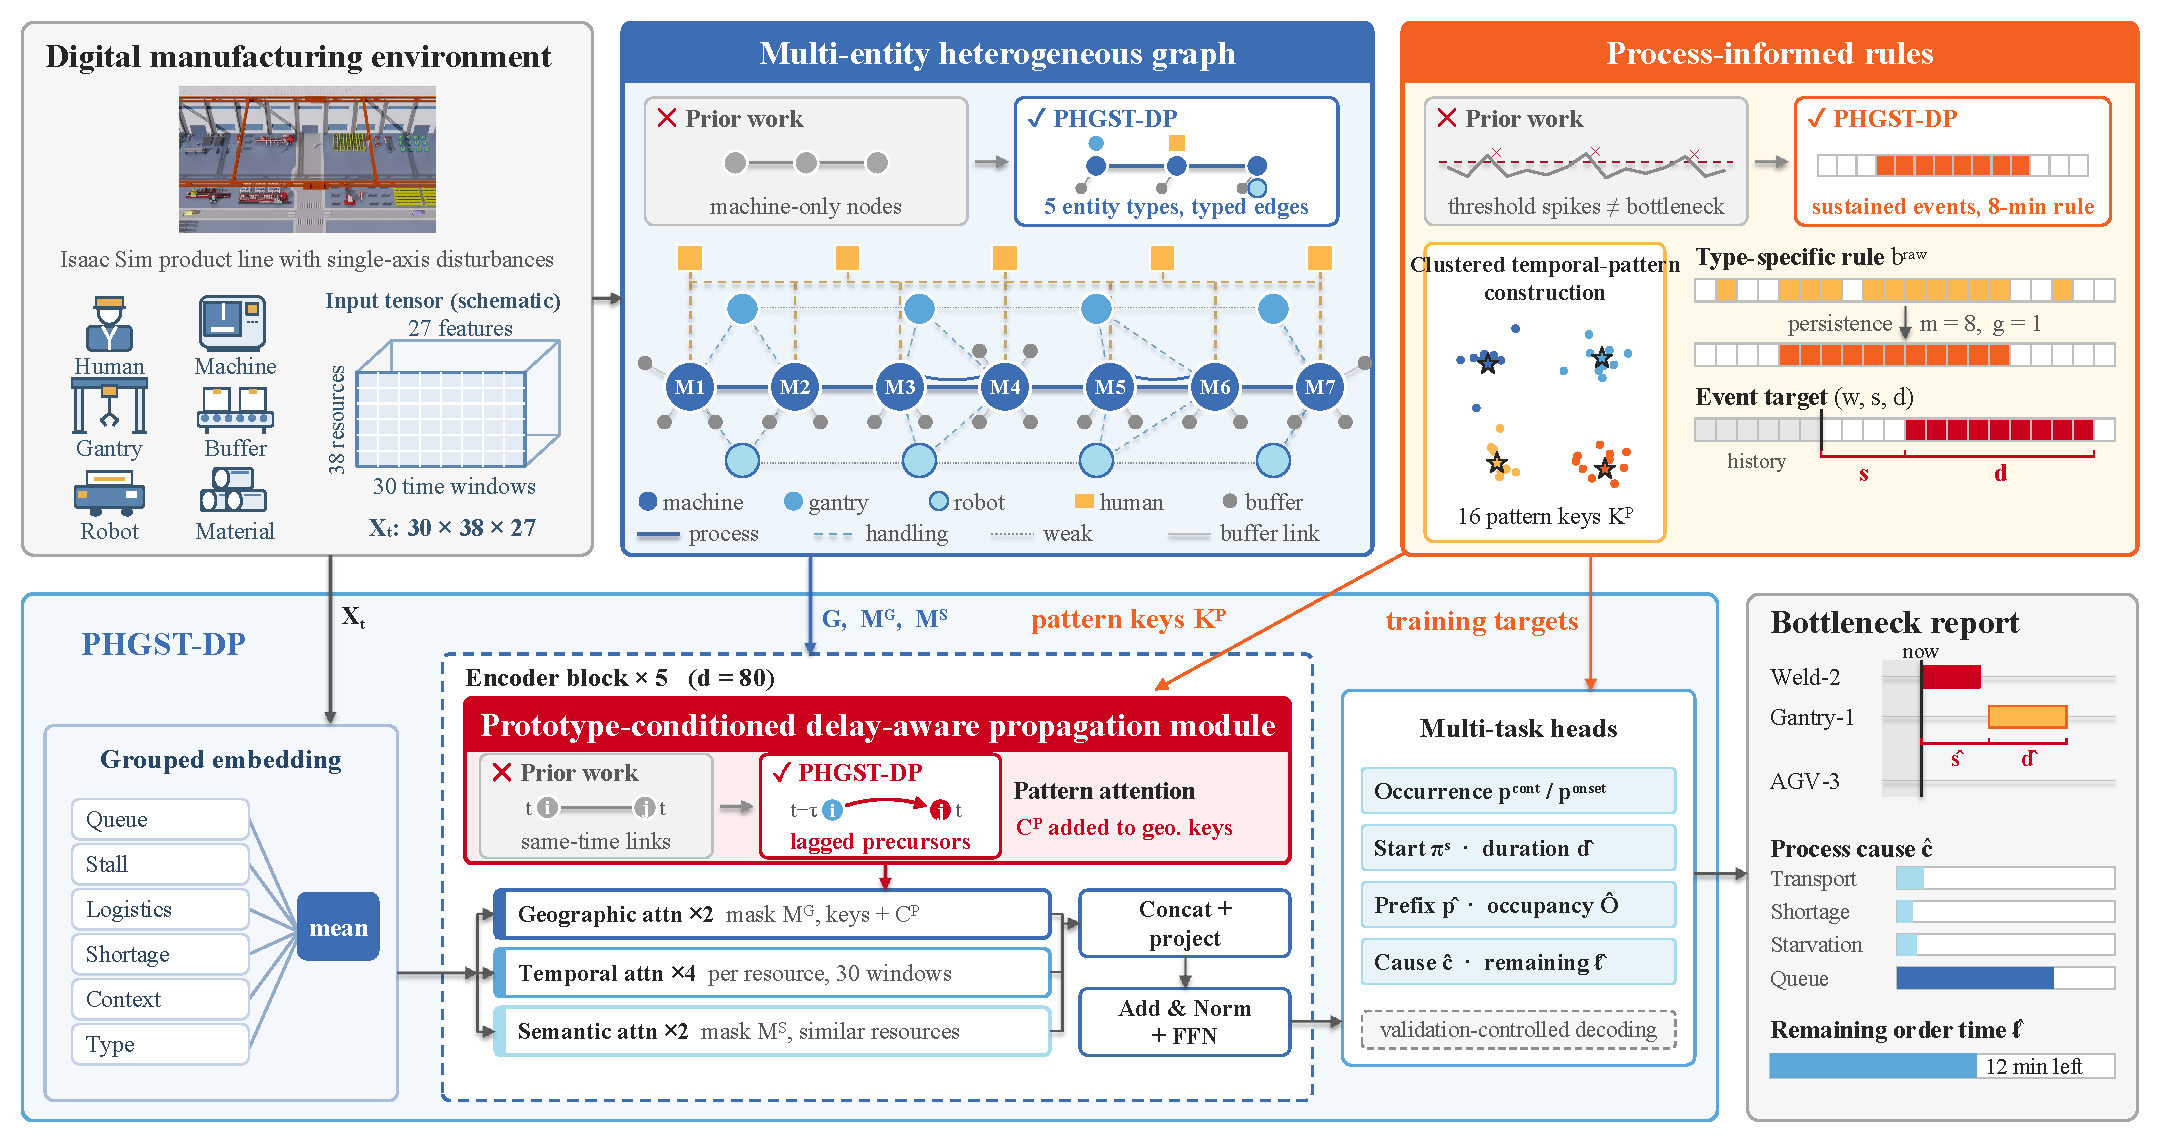
\includegraphics[width=\textwidth]{figures/fig_method_final.pdf}
\caption{Overview of the problem formulation and the PHGST-PD method.}
\label{fig:method-framework}
\end{figure*}

\subsection{Production system and resource relations}

The production system comprises multiple interacting resource entities. We represent this multi-entity environment as a heterogeneous process--logistics graph with resource-specific node types and typed relations. This representation distinguishes the resources that receive bottleneck-event supervision from the contextual resources that influence how constraints form and propagate.

\subsubsection{Production task and resource entities}

We consider a shared water-pipe production line represented in an open-workspace factory environment, with cutting, grooving, spot welding, root welding, surface welding, and finishing operations. In this study, a workstation denotes a processing or assembly unit, including automated equipment and manually operated workbenches. The process is coupled with storage, gantry handling, transport-robot delivery, and worker service. The graph implementation represents the primary process backbone with seven workstation nodes because parallel workbench and rotary-welding resources are retained as separate stations. Each production episode contains one order of ten products, and the nominal controller admits at most five products as concurrent WIP. It coordinates admission, process precedence, resource availability, and handling tasks; bottleneck prediction observes this controlled process but does not replace the controller.

Let the complete resource set be
\begin{equation}
\mathcal{R}=\mathcal{R}^{m}\cup\mathcal{R}^{g}\cup
\mathcal{R}^{a}\cup\mathcal{R}^{h}\cup\mathcal{R}^{b},
\end{equation}
where the superscripts denote workstations, gantries, transport robots, workers, and buffers. The retained graph contains 38 nodes: 7 workstation nodes, 4 gantries, 4 transport robots, 5 workers, and 18 buffers. Material is not represented as a separate graph node; its state enters through shortage propagation, inbound waiting, affiliated-buffer occupancy, and other material-flow channels attached to the affected resources. These entities have different operational meanings. A workstation transforms a product, a gantry or transport robot moves a product between locations, a worker provides labour-dependent service, and a buffer stores intermediate products. The event-supervised target set is
\begin{equation}
\mathcal{S}=\mathcal{R}^{m}\cup\mathcal{R}^{g}\cup\mathcal{R}^{a}.
\end{equation}
Worker and buffer nodes remain in the observation graph because labour availability and storage occupancy influence other resources, but the current implementation does not assign them station-event targets.

\subsubsection{Heterogeneous process--logistics graph}

The production system is represented as a weighted undirected graph
\begin{equation}
G=(\mathcal{R},E,A),\qquad
E=E^{p}\cup E^{f}\cup E^{b}\cup E^{l}\cup E^{w},
\end{equation}
where $E^{p}$ follows the seven-station process chain, $E^{f}$ connects parallel workstations belonging to the same equipment family, $E^{b}$ links storage buffers to affiliated workstations, $E^{l}$ links handling agents to workstation resources, and $E^{w}$ provides weak links among gantries or among transport robots. The implemented edge weights are $1.0$, $0.8$, $0.6$, $0.5$, and $0.3$ for these five relation groups, respectively, and every node receives a self-loop of weight $1.0$.

The graph preserves resource-type distinctions and specifies possible channels through which material flow, service delay, and congestion can propagate. Process edges encode downstream dependency; buffer edges expose storage-mediated blockage or starvation; and logistics edges connect a delayed workstation input to the handling resources that can cause it. This distinction is important because two nodes may be structurally close but have different feature semantics, while two structurally distant nodes may exhibit similar operating trajectories. Section~\ref{sec:method} therefore derives both geographic and semantic attention masks from $G$ and the training trajectories.

\subsection{State representation and prediction targets}

The resource graph is observed through fixed production windows and paired with process-informed event and auxiliary targets. The following definitions align the historical input, future bottleneck interval, process cause, and order-level progress within one prediction sample.

\subsubsection{Windowed production state}

Raw factory-model events are sampled at logical-second resolution and aggregated into non-overlapping windows of $\Delta=60$\,s. For resource $n$ and window $t$, the state $x_{t,n}\in\mathbb{R}^{27}$ contains twenty-one operational variables, five resource-type indicators, and one labour-saturation context variable. The operational variables cover queue and occupancy, activity and waiting, blockage and starvation, downtime, inter-departure variability, upstream/downstream interaction, route and inbound delay, shortage propagation, affiliated-buffer occupancy, operating variation context, and two turning-point/momentary indicators. Labour saturation is computed from the worker states and broadcast only to workstation nodes. The bottleneck score used by the offline aggregation pipeline is deliberately excluded from $x_{t,n}$ to avoid leaking a supervision signal into the predictor.

\begin{table}[pos=t]
\centering
\caption{Semantic groups of the 27-dimensional resource state.}
\label{tab:feature-groups}
\scriptsize
\setlength{\tabcolsep}{3pt}
\renewcommand{\arraystretch}{1.12}
\begin{tabularx}{\columnwidth}{@{}l c >{\raggedright\arraybackslash}X@{}}
\toprule
Group & Dim. & Representative information \\
\midrule
Queue & 4 & Queue length, waiting, occupancy, growth \\
Stall & 6 & Blocked/starved time, stop, availability, coupling \\
Logistics & 4 & Departure variation, route/inbound delay, buffer \\
Shortage & 1 & Material-shortage propagation \\
Context & 7 & Activity, duration, time gap, operating variation, turning state, labour \\
Type & 5 & Workstation, gantry, worker, robot, buffer \\
\bottomrule
\end{tabularx}
\end{table}

Given $T_{\mathrm{in}}=30$ historical windows over $N$ resources, the model input is
\begin{equation}
X_t=\left[x_{\tau,n}\right]_
{\substack{\tau=t-T_{\mathrm{in}},\ldots,t-1\\n=1,\ldots,N}}
\in\mathbb{R}^{T_{\mathrm{in}}\times N\times 27}.
\end{equation}
The future label grid contains $H_{\mathrm{label}}=30$ one-minute windows. Within this grid, the admissible event onset $H_{\mathrm{start}}$ is varied between experimental settings. Separating the thirty-minute label grid from the onset cap allows an event to begin up to fifteen minutes ahead while retaining enough future windows to satisfy the eight-window persistence requirement.

\subsubsection{Process-informed supervision for bottleneck events}

A bottleneck label must distinguish a production-relevant constraint from ordinary activity or travel. For each supervised resource, the implementation first applies a type-dependent rule
\begin{equation}
b^{\mathrm{raw}}_{t,n}=\Phi_{\rho(n)}(x_{t,n},X_t)\in\{0,1\},
\end{equation}
where $\rho(n)$ is the resource type. For a workstation, $\Phi_m$ combines queue accumulation with blocked or starved time, coupled upstream/downstream evidence, shortage propagation, inbound or route delay, downtime, and labour-related waiting. An operating variation flag alone is insufficient: it must coincide with queue, stall, or unavailability evidence. For a gantry, a hot state requires route or inbound delay with stalling, or a stop/unavailable state. For a transport robot, inbound waiting must coincide with stalling, or the robot must be frozen/stopped; normal route travel is not considered a bottleneck.

The raw binary grid is converted into sustained occupancy. In the retained configuration, runs shorter than $m=8$ windows are removed first; an internal cold gap of at most $g=1$ window is then filled when it lies between retained hot regions. Denoting short-run removal by $\mathcal{D}_{m}$ and gap filling by $\mathcal{F}_{g}$, the implemented legacy order is
\begin{equation}
o_{:,n}=\mathcal{F}_{g}\!\left(\mathcal{D}_{m}
\left(b^{\mathrm{raw}}_{:,n}\right)\right).
\end{equation}
This persistence requirement rejects isolated threshold crossings. The occupancy grid $o$ is an offline supervision target. At a forecast origin $t$, the model instead uses a history-only state $h_{t-1,n}$ computed from the observed prefix $x_{0:t,:,:}$, with no observations at or after $t$. Any persistence check used to construct this historical state is evaluated on that prefix only; internal-gap filling cannot use a future hot segment. The historical state is therefore distinct from the retrospective label $o_{t-1,n}$. It should not be confused with the offline event CSV, whose score-event merge can retain a one-window event; PHGST-PD training targets are generated from the operational occupancy grid and use the eight-window criterion.

For a history ending immediately before window $t$, the primary target for station $n$ is
\begin{equation}
y_{t,n}^{\mathrm{evt}}=(w_{t,n},s_{t,n},d_{t,n}),
\end{equation}
where $w_{t,n}$ indicates that an eligible run exists, $s_{t,n}$ is its onset offset, and $d_{t,n}$ is its length within the future grid. If the history-only state $h_{t-1,n}=1$ and the future run begins at offset zero, the event is \emph{ongoing}; its future remainder may be shorter than eight windows because the full event already satisfied persistence before the observation boundary. Otherwise, a run with $s_{t,n}>0$ is \emph{upcoming} and must satisfy the configured minimum duration. If several runs are available for one station, the longest eligible run is selected rather than the earliest run.

Algorithm~\ref{alg:targets} consolidates the complete supervision pipeline, from type-dependent state evidence to persistent events, cause targets, regime context, and order-level remaining time. Worker and buffer nodes contribute contextual observations but are omitted from station-event decoding because they are not in $\mathcal{S}$.

\begin{algorithm*}[t]
\caption{Process-informed supervision and regime-context construction.}
\label{alg:targets}
\KwIn{episode trajectories $\mathcal{E}$; resource types $\rho$; supervised set $\mathcal{S}$; $T_{\mathrm{in}}$; $H_{\mathrm{label}}$; $H_{\mathrm{start}}$; $m{=}8$; $g{=}1$}
\KwOut{causal samples $\mathcal{D}=\{X_t,O_t,Y_t^{\mathrm{evt}},c_t,\ell_t,r_t\}$}
$\mathcal{D}\leftarrow\varnothing$\;
\ForEach{completed, reset-free episode $e\in\mathcal{E}$}{
  \tcp{Stage 1: synchronize heterogeneous observations}
  aggregate raw streams into non-overlapping $60$,s windows\;
  align resource states by identifier and append type/context channels\;
  preserve the episode boundary and compute jobs remaining\;
  \tcp{Stage 2: construct the persistent occupancy grid}
  \ForEach{$n\in\mathcal{S}$ and window $u$}{
    $b^{\mathrm{raw}}_{u,n}\leftarrow\Phi_{\rho(n)}(x_{u,n})$ using queue, stall, availability, shortage, and logistics evidence\;
  }
  \ForEach{$n\in\mathcal{S}$}{
    $o_{:,n}\leftarrow\mathcal{F}_{g}(\mathcal{D}_{m}(b^{\mathrm{raw}}_{:,n}))$ \tcp*{drop short runs, then fill gaps}
  }
  \tcp{Stage 3: derive process cause and regime context}
  \ForEach{window $u$ and resource $n$}{
    assign $r_{u,n}$ by the deterministic cause-aligned state rules\;
  }
  \ForEach{window $u$ containing reportable hot evidence}{
    assign $c_u$ by the priority shortage $\succ$ delay $\succ$ queue $\succ$ blockage\;
    set the cause-loss weight to $1$ only when $c_u\in\mathcal{C}$\;
  }
  \tcp{Stage 4: instantiate one causal forecasting sample}
  \For{$t\leftarrow T_{\mathrm{in}}$ \KwTo episode completion}{
    $X_t\leftarrow x_{t-T_{\mathrm{in}}:t,:,:}$ and $O_t\leftarrow o_{t:t+H_{\mathrm{label}},:}$\;
    compute $h_{t-1}$ from the observed prefix $x_{0:t,:,:}$ only \tcp*{no retrospective occupancy supplied to inference}
    \ForEach{$n\in\mathcal{S}$}{
      $(s,d)\leftarrow$ longest hot run of $O_{t,:,n}$ whose onset is within $H_{\mathrm{start}}$\;
      \eIf{$h_{t-1,n}=1$ and $s=0$}{
        $(w_{t,n},s_{t,n},d_{t,n})\leftarrow(1,0,d)$ \tcp*{ongoing remainder}
      }{
        \eIf{$0<s\le H_{\mathrm{start}}$ and $d\ge m$}{
          $(w_{t,n},s_{t,n},d_{t,n})\leftarrow(1,s,d)$ \tcp*{upcoming event}
        }{
          $(w_{t,n},s_{t,n},d_{t,n})\leftarrow(0,0,0)$\;
        }
      }
    }
    $\ell_t\leftarrow$ future one-minute windows until all jobs finish, clipped by the prediction cap\;
    append $(X_t,O_t,Y_t^{\mathrm{evt}},c_{t-1},\ell_t,r_{t-1})$ to $\mathcal{D}$\;
  }
}
\Return $\mathcal{D}$\;
\end{algorithm*}

\subsubsection{Cause and order-level targets}

Station events identify where and when production is constrained, but intervention also requires a process explanation. The aggregation pipeline assigns a window-level cause through a fixed evidence priority: material shortage, transport delay, queue buildup, and downstream blockage. The label is inferred from measured shortage, inbound/route delay, queue, and blocked variables; it is not copied from the injected operating variation dimension.

The reported cause set is
\begin{equation}
\begin{aligned}
\mathcal{C}=\{&
\text{material shortage},\text{transport delay},\\
&\text{queue buildup},\text{downstream blockage}\}.
\end{aligned}
\end{equation}
The order-level target $\ell_t$ is the number of future one-minute windows until all jobs are complete under the configured prediction cap. It provides a line-level estimate of production consequence that complements the station-level event report.

The cause-assignment stage of Algorithm~\ref{alg:targets} applies this priority to each reportable hot window. The same algorithm distinguishes these cause targets from deterministic regime identifiers: the former supervise the graph-level explanation head, whereas the latter only condition the station-event representation.

\subsection{Multi-task prediction formulation}

The complete prediction problem is the mapping
\begin{equation}
f_{\theta}:(X_t,G)\longmapsto
\left(
\{\hat w_{t,n},\hat s_{t,n},\hat d_{t,n}\}_{n\in\mathcal{S}},
\hat c_t,\hat\ell_t
\right).
\end{equation}
This formulation differs from forecasting a bottleneck score. The outputs jointly describe the affected resource, event onset and persistence, process explanation, and expected order impact. The method in Section~\ref{sec:method} parameterizes $f_{\theta}$ with a delay-aware heterogeneous spatiotemporal encoder and multiple task heads.

The delayed-propagation challenge is contained in this mapping rather than introduced as an additional label. For an upcoming event at target resource $j$, predictive evidence may occur at another resource $i$ and at an earlier history offset $\tau$. The model must therefore learn associations of the form
\begin{equation}
(x_{t-\tau,i},\,i\!\rightarrow\!j)\longmapsto y^{\mathrm{evt}}_{t,j},
\qquad \tau>0,
\end{equation}
where $i\!\rightarrow\!j$ denotes a possible process or logistics route, not a proven physical causal path. This formulation motivates conditioning cross-resource interaction on recurrent historical patterns while evaluating success only through the future event report.

Two event criteria are distinguished. A station-level hit requires that the predicted resource equal the labelled resource. A stricter report-level true positive additionally requires
\begin{equation}
|\hat{s}_{t,n}-s_{t,n}|\leq\epsilon_s,\qquad
\epsilon_s=3~\mathrm{min}.
\end{equation}
Occurrence precision, recall, and F1 quantify the coverage and reliability of alarms. Start, duration, and remaining-time errors are conditional or regression measures and cannot compensate for a missed station event. Ongoing and upcoming recalls are therefore reported separately: the latter is the direct measure of whether the model provides warning before the bottleneck becomes visible at the target station.

%% ========================================================================
\section{Methodology} \label{sec:method}
%% ========================================================================

\subsection{Method overview}

PHGST-PD is organized around the three contributions established in Section~\ref{sec:intro}. First, an open-workspace factory model developed for NVIDIA Isaac Sim, a heterogeneous factory graph, and grouped embedding integrate workstation, worker, material-flow, buffer, gantry, and transport evidence. Second, process-informed supervision and temporal pattern clustering produce traceable event and cause supervision, deterministic regime context, and recurrent operating-pattern prototypes. Third, the propagation-delay-aware module uses those prototypes to organize lagged cross-resource interaction. The complete information flow is
\begin{equation}
\begin{aligned}
\text{factory model}&\rightarrow\text{window/event construction}\\
&\rightarrow\text{factory graph}\rightarrow\text{joint prediction}.
\end{aligned}
\end{equation}
The first two stages create reproducible observations and targets. The latter two parameterize the mapping $f_\theta$ defined in Section~\ref{sec:problem}.

Figure~\ref{fig:model-architecture} presents the PHGST-PD model architecture. The multi-entity history is partitioned into six semantic feature groups and combined with temporal, graph-Laplacian, and node-identity embeddings. Temporal pattern clustering supplies a fixed prototype bank, and the propagation-delay-aware module uses that bank to condition geographic keys so that recurrent precursors can influence cross-resource interaction after a delay. Station-level and graph-level heads then decode occurrence, onset, duration, future occupancy, process cause, and remaining order time.

\begin{figure*}[t]
\centering
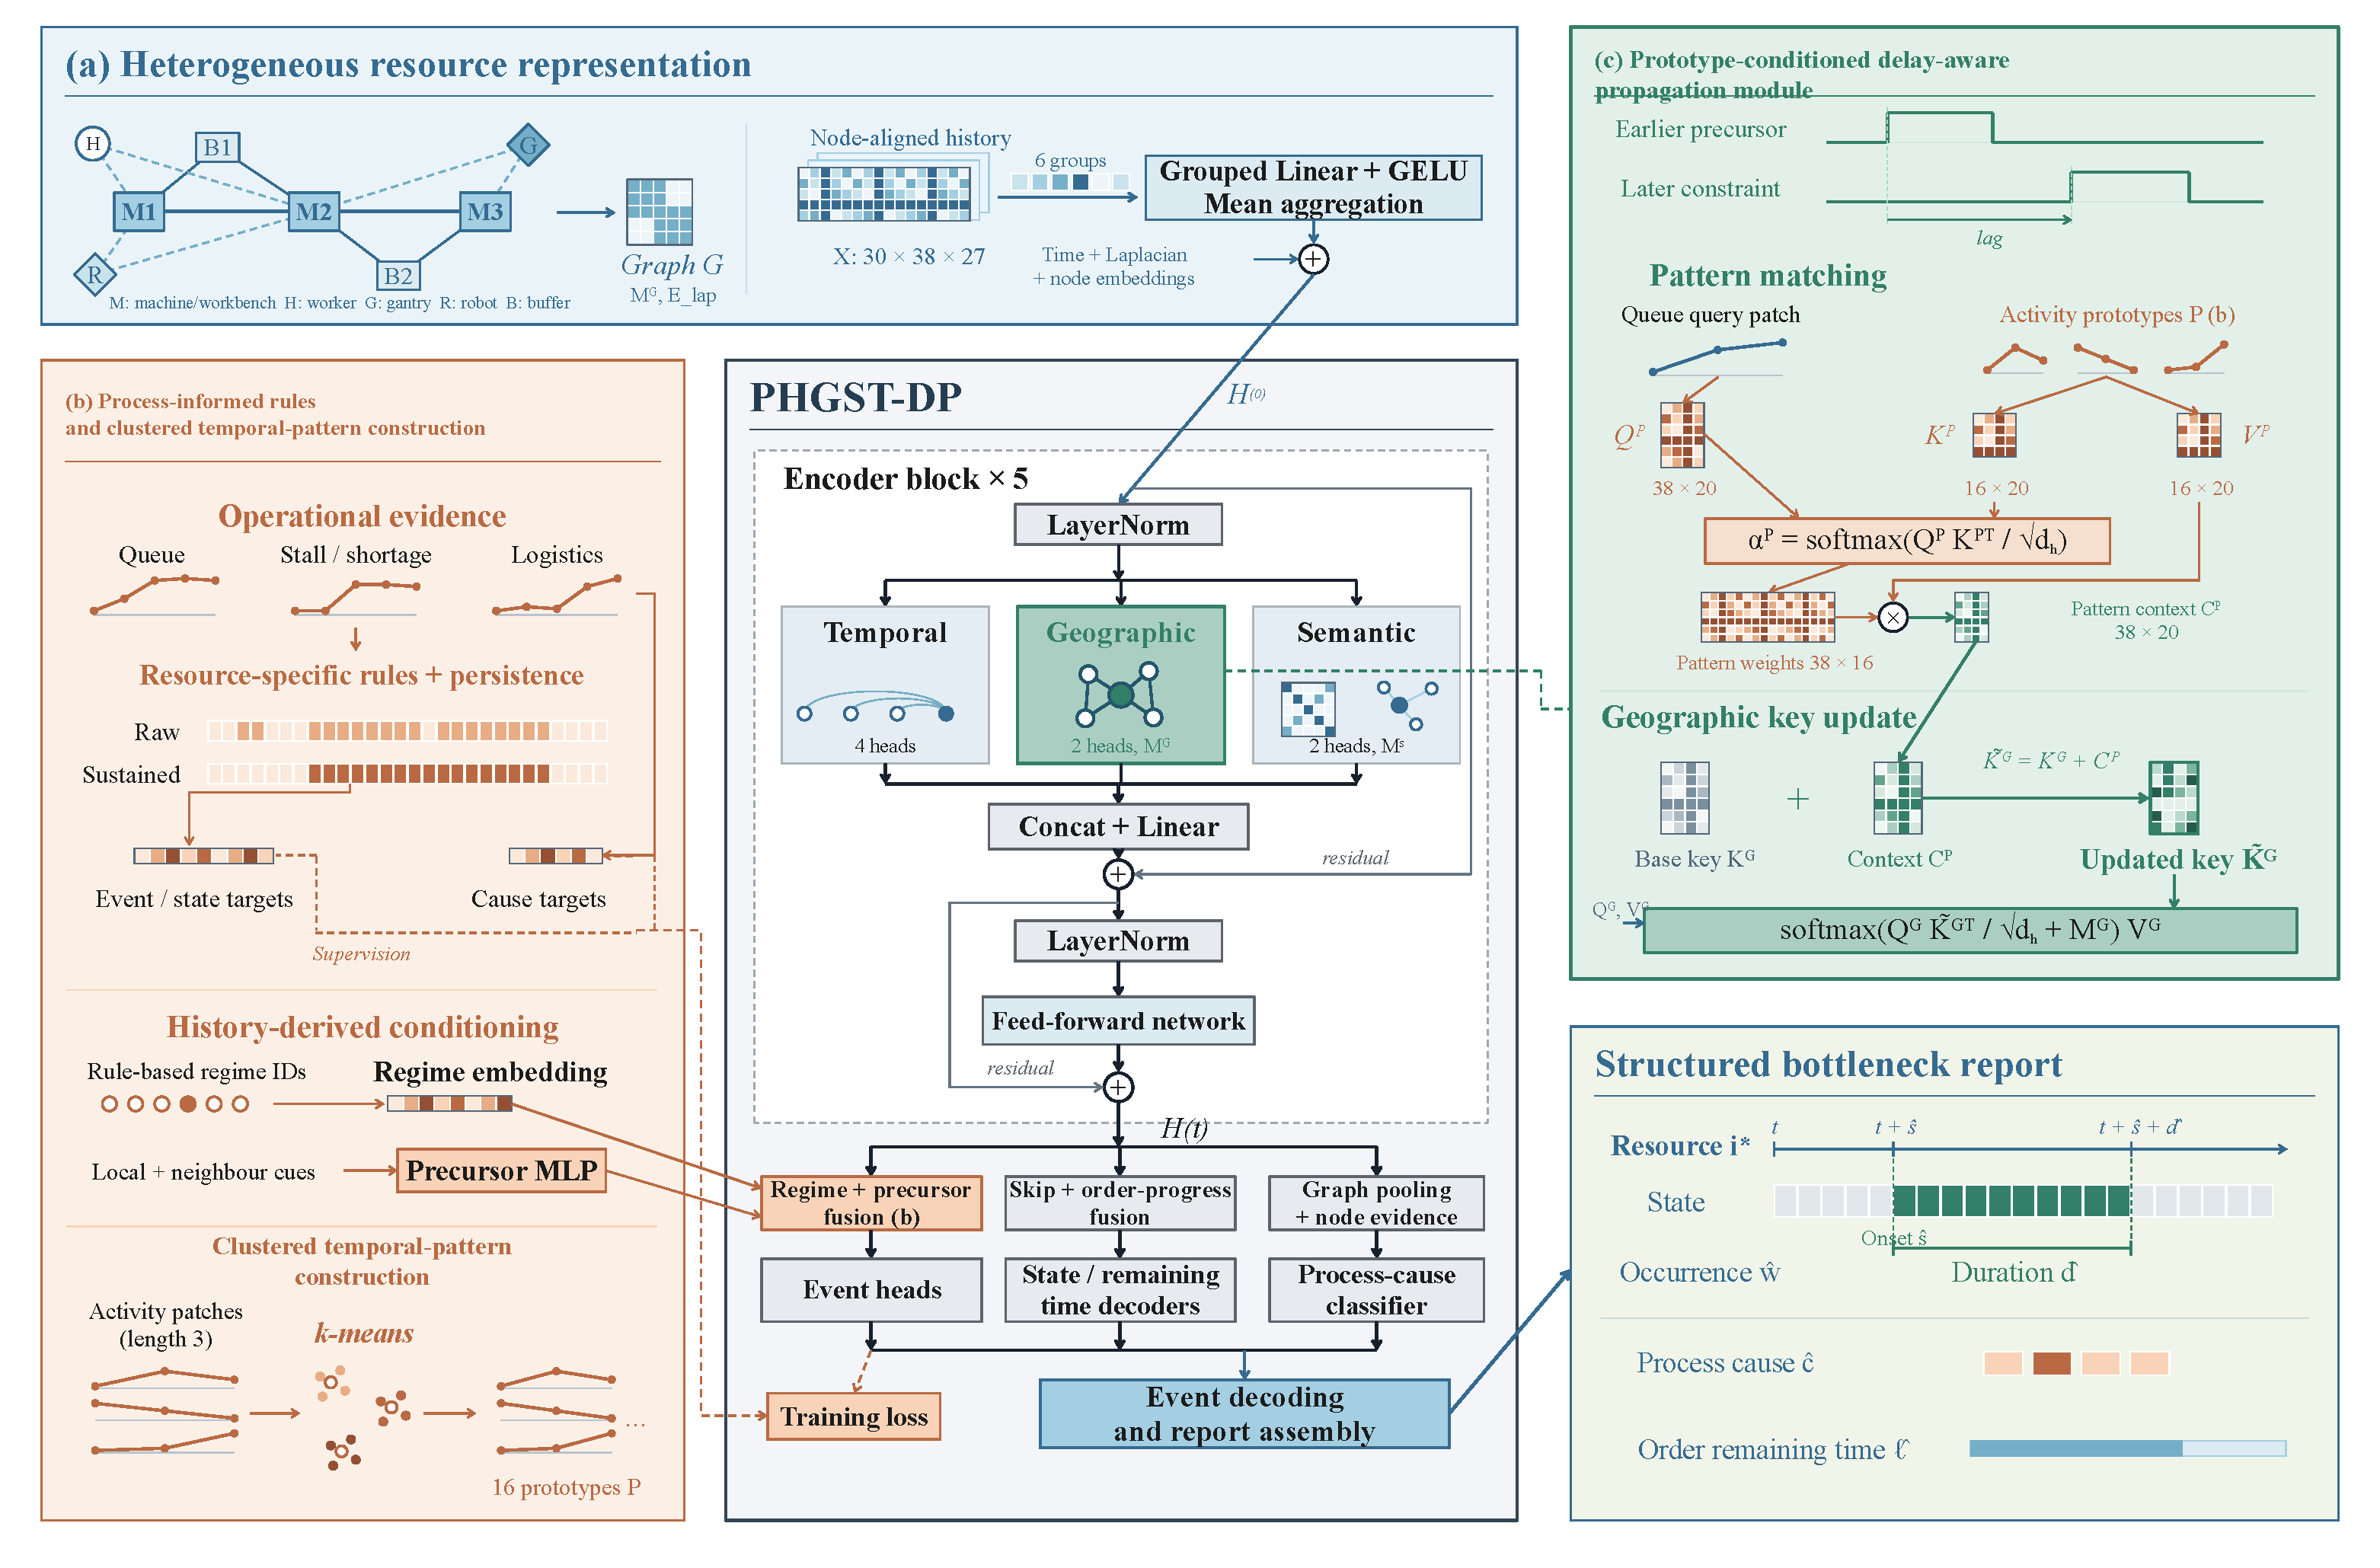
\includegraphics[width=\textwidth]{figures/fig_model_final.pdf}
\caption{Architecture of PHGST-PD.}
\label{fig:model-architecture}
\end{figure*}

Algorithm~\ref{alg:phgst-train} gives the end-to-end learning and model-selection procedure around that architecture. It makes explicit which quantities are fitted from training episodes, how validation controls checkpoint and threshold selection, and when the held-out episodes are first evaluated. Algorithm~\ref{alg:phgst-predict} then expands one complete PHGST-PD forward and report-generation pass.

\begin{algorithm*}[t]
\SetAlFnt{\small}
\SetAlCapFnt{\small}
\SetAlCapNameFnt{\small\bfseries}
\SetInd{0.6em}{1.0em}
\caption{End-to-end PHGST-PD training, selection, and held-out evaluation.}
\label{alg:phgst-train}
\KwIn{raw episodes $\mathcal{E}$; factory relations $G$; onset caps $\mathcal{H}=\{5,10,15\}$; candidate thresholds $\mathcal{T}$}
\KwOut{frozen event model $\theta^{\star}$, remaining-time head $\psi^{\star}$, threshold $\tau^{\star}$, held-out reports}
\BlankLine
\textbf{Stage 1: leakage-controlled data and fixed structural context}\;
split $\mathcal{E}$ by episode into $\mathcal{E}_{\mathrm{tr}},\mathcal{E}_{\mathrm{val}},\mathcal{E}_{\mathrm{te}}$\;
construct causal samples with Algorithm~\ref{alg:targets} independently inside each episode\;
fit all feature/target scalers on $\mathcal{E}_{\mathrm{tr}}$; reuse them unchanged for $\mathcal{E}_{\mathrm{val}}$ and $\mathcal{E}_{\mathrm{te}}$\;
obtain $(A,M^{G},M^{S},E_{\mathrm{lap}})$ from Algorithm~\ref{alg:graph-masks} and $K^{P}$ from Algorithm~\ref{alg:pattern-bank}\;
freeze every data-derived structural quantity before neural-parameter optimization \tcp*{masks and prototypes stay fixed}
\BlankLine
\textbf{Stage 2: curriculum learning of shared representations and event-related heads}\;
initialize $\theta$ from the documented prefix-supervised checkpoint\;
\ForEach{$H_{\mathrm{start}}\in\mathcal{H}$ in curriculum order}{
  warm-start the current onset cap from the preceding retained checkpoint when available\;
  \For{epoch $=1,\ldots,E_1$ until patience is exhausted}{
    \ForEach{oversampled training minibatch $B$}{
      $(\widehat{Y}^{\mathrm{evt}},\hat O,\hat c,\hat\ell)\leftarrow\mathrm{PHGSTPDForward}_{\theta}(B,A,M^{G},M^{S},K^{P})$\;
      evaluate the event, occupancy, cause, reconstruction, contrastive, and remaining-time losses, then update $\theta$\;
    }
    decode $\mathcal{E}_{\mathrm{val}}$ with Algorithm~\ref{alg:phgst-predict} for every $\tau\in\mathcal{T}$\;
    retain the checkpoint--threshold pair that passes the precision/recall gates and maximizes station F1\;
  }
}
freeze the selected stage-1 parameters and threshold as $(\theta^{\star},\tau^{\star})$ \tcp*{event reports locked hereafter}
\BlankLine
\textbf{Stage 3: remaining-time specialization without changing event reports}\;
freeze the encoder and all event, occupancy, and cause heads\;
initialize the rate-augmented remaining-time head $\psi$ from $\theta^{\star}$\;
\For{epoch $=1,\ldots,E_2$ until validation loss stops improving}{
  update only $\psi$ using progress-weighted remaining-time loss\;
}
freeze $\psi^{\star}$; do not retune $\tau^{\star}$\;
\BlankLine
\textbf{Stage 4: held-out evaluation after all choices are frozen}\;
run Algorithm~\ref{alg:phgst-predict} on $\mathcal{E}_{\mathrm{te}}$ using $(\theta^{\star},\psi^{\star},\tau^{\star})$\;
\Return frozen models, threshold, and held-out reports \tcp*{test episodes never re-enter selection}
\end{algorithm*}

\subsection{Data preparation and graph instantiation}

Section~\ref{sec:problem} defines the entities, graph relations, and prediction targets. This stage describes only how those formal objects are instantiated for PHGST-PD: factory-model trajectories are converted into a synchronized resource--time tensor, aligned supervision targets, and the structural and semantic masks required by the encoder.

\subsubsection{Open-workspace factory model}

Data are collected using an open-workspace factory model developed for NVIDIA Isaac Sim. The model represents the water-pipe line, resource layout, storage locations, and handling activities. At every logical second, the collector records the episode configuration, active operating variation, resource-state transitions, job traces, buffer events, transport tasks, and material inventory. These streams are synchronized by episode and logical time, allowing a downstream event to be traced back through the states that preceded it. A known model implementation defect can trigger a deadlock reset that is not part of the intended production process and does not represent a physical production condition. Episodes affected by this defect are treated as invalid model records and removed; valid episodes are exported after all ten products complete.

Formal single-axis collection activates one operating variation dimension at intensity $I=1.0$ while leaving the other dimensions nominal:
\begin{itemize}
 \item[$\bullet$] \textbf{Workstation operating variation} increases processing-time variation, lowers successful operation probability, disables selected workstations, and inserts temporary workstation-fault pulses.
 \item[$\bullet$] \textbf{Worker operating variation} reduces the workforce from five to three, increases task-time variation, and inserts temporary leave periods.
 \item[$\bullet$] \textbf{Logistics operating variation} reduces transport robots from four to two, slows gantry motion, and inserts handling freezes that include an AGV freeze.
 \item[$\bullet$] \textbf{Material operating variation} temporarily hides flange or elbow kits and introduces additional shortage pulses for selected stock-keeping units.
\end{itemize}
The temporary workstation, worker, and logistics pulses last at least ten logical minutes. This design does not assume that the injected dimension is the final bottleneck cause. Its purpose is to produce traceable perturbations whose operational consequences can emerge at different resources and times.

\subsubsection{Multi-entity aggregation and target instantiation}

The second stage converts heterogeneous raw logs into a common resource--time grid. Statistics are aggregated over non-overlapping one-minute windows and aligned by resource identifier. Missing resource states are completed through the export pipeline, type one-hot variables are appended, and labour saturation is recomputed from the available worker nodes. The resulting tensor contains 38 resource nodes and 27 channels in the retained dataset. Episode boundaries are preserved throughout sliding-window generation, preventing a history from combining observations from two production runs.

The pipeline instantiates the supervision defined in Section~\ref{sec:problem} from each aggregated episode, producing aligned occurrence, onset, duration, occupancy-grid, prefix, process-cause, and remaining-time targets. The retained configuration derives event targets from operational states rather than the exported bottleneck-score column, preventing the model from solving the task by reproducing an aggregation score.

Three different clustering-related objects are kept conceptually separate. First, the offline aggregation tools can produce station- and window-level $K=8$ k-means descriptors for exploratory regime analysis. Second, the training dataset derives cause-aligned regime identifiers by deterministic rules and can use them for representation conditioning and contrastive regularization. Third, the temporal pattern clustering component fits short temporal patches to create the recurrent prototype bank. Temporal pattern clustering fits the prototype bank. The propagation-delay-aware module then matches recent patches to these prototypes and adds the resulting context to geographic attention. The offline cluster-prediction loss has weight zero, and no cluster index defines the bottleneck ground truth; event labels are produced only by the process rules and persistence filter above.

\subsubsection{Heterogeneous factory graph and attention masks}

The weighted adjacency $A$ follows the relation definitions in Section~\ref{sec:problem}. Floyd--Warshall shortest-path computation converts nonzero edges into hop distances $D^{\mathrm{hop}}$. The geographic mask is
\begin{equation}
M^G_{ij}=
\begin{cases}
0, & D^{\mathrm{hop}}_{ij}<\delta_G,\\
-\infty, & \text{otherwise},
\end{cases}
\qquad \delta_G=4,
\end{equation}
so a node attends only to resources fewer than four hops away in geographic attention. This mask allows information to cross more than one process or logistics edge while excluding globally unrelated nodes.

Geographic proximity alone cannot capture parallel or substitutable resources with similar behaviour. A semantic distance matrix is therefore computed from training trajectories. The feature channels of each node are first averaged to form a scalar trajectory $\bar x_{:,i}$, after which
\begin{equation}
D^{\mathrm{sem}}_{ij}
=1-\mathrm{corr}(\bar{x}_{:,i},\bar{x}_{:,j}).
\end{equation}
For each node, the five nearest trajectories are unmasked in $M^S$; all others are suppressed. This implementation uses Pearson correlation distance as a short-episode substitute for the dynamic-time-warping distance used in traffic PDFormer. Finally, the nontrivial eigenvectors of the normalized graph Laplacian provide an eight-dimensional structural position for every resource. The exact graph-and-mask instantiation invoked during training is isolated in Algorithm~\ref{alg:graph-masks}. All trajectory-dependent quantities in this procedure are computed from the training split only.

\subsection{Delay-aware heterogeneous spatiotemporal encoding}

The encoder first preserves the distinct semantics of heterogeneous observations through grouped embedding and then models temporal evolution, graph propagation, and behavioural similarity. The propagation-delay-aware module further links current resource states with recurrent precursor patterns whose effects emerge later in the production process.

\subsubsection{Grouped heterogeneous state embedding}

A single linear projection would combine all 27 channels without explicitly distinguishing the semantics of queue length, downtime, type codes, and shortage evidence. The grouped token embedding instead partitions the channels into queue, stall, logistics, shortage, context, and type groups. Each group $q$ has an independent affine projection and GELU activation:
\begin{equation}
e^{(q)}_{t,n}=\mathrm{GELU}
\left(W_q x^{(q)}_{t,n}+b_q\right).
\end{equation}
The six group embeddings are mean-pooled, rather than concatenated as separate tokens:
\begin{equation}
e_{t,n}=\frac{1}{6}\sum_{q=1}^{6}e^{(q)}_{t,n}.
\end{equation}
This operation maps heterogeneous evidence to a common latent space and gives each feature group equal weight in the pooling step, regardless of its channel count.

The initial representation combines grouped evidence with temporal, structural, and identity information:
\begin{equation}
H^{(0)}=E_{\mathrm{group}}(X_t)+
E_{\mathrm{time}}+E_{\mathrm{lap}}(G)+E_{\mathrm{node}}.
\end{equation}
$E_{\mathrm{time}}$ is sinusoidal, $E_{\mathrm{lap}}$ projects the graph eigenvectors, and $E_{\mathrm{node}}$ is a learned resource-identity embedding. Day-of-week and time-of-day embeddings are disabled because an episode is driven by order progress and operating variations rather than calendar periodicity.

\subsubsection{Propagation-delay-aware module}

The propagation-delay-aware module must distinguish three dependencies: evolution of one resource through time, propagation through the process--logistics graph, and similarity between resources that need not be adjacent. Each encoder block therefore allocates separate attention heads to temporal, geographic, and semantic attention. For an attention branch $b\in\{T,G,S\}$,
\begin{equation}
\mathrm{Attn}_{b}(Q_b,K_b,V_b;M_b)
=\mathrm{softmax}\!\left(
\frac{Q_bK_b^\top}{\sqrt{d_h}}+M_b
\right)V_b ,
\end{equation}
where temporal attention has no cross-node mask, geographic attention uses $M^G$, and semantic attention uses $M^S$.

Temporal pattern clustering supplies the data-derived keys used by the propagation-delay-aware module. In the retained implementation, the prototype bank is fitted by applying k-means with sixteen centres to length-three patches of the configured activity channel (\texttt{active\_pct\_s}), whereas online query patches use the first model-output channel (\texttt{queue\_length\_s}). Let $P_{t,n}$ denote a queue query patch and $K^P$ the learned activity-pattern centres. Prototype matching computes
\begin{equation}
C^P_{t,n}=
\mathrm{softmax}\!\left(
\frac{Q^P(P_{t,n})K^P(K^P)^\top}{\sqrt{d_h}}
\right)V^P(K^P).
\end{equation}
The resulting cross-channel pattern context is added to the geographic key before geographic attention is evaluated. Spatial interaction therefore depends on node proximity and the learned association between current queue evolution and recurrent activity prototypes. The mechanism does not use a Fourier transform. Algorithm~\ref{alg:pattern-bank} specifies the training-only extraction and Lloyd-update procedure used to obtain this prototype bank.

For encoder block $l$, the three branches are
\begin{equation}
\begin{aligned}
H_T^{(l)}&=\mathrm{Attn}_T(H^{(l-1)}),\\
H_G^{(l)}&=\mathrm{Attn}_G(H^{(l-1)},M^G,C^P),\\
H_S^{(l)}&=\mathrm{Attn}_S(H^{(l-1)},M^S).
\end{aligned}
\end{equation}
Their outputs are concatenated, projected, and processed by pre-normalized residual and feed-forward layers. The retained configuration uses five blocks with latent dimension 80. It allocates four temporal heads, two geographic heads, and two semantic heads; these are separate branches rather than one undifferentiated eight-head attention module.

\subsection{Multi-task bottleneck prediction and optimization}

The shared spatiotemporal representation is converted into station-level event reports and graph-level explanatory outputs. The prediction heads, joint objective, and validation-controlled decoder form a single sequence from latent representation to the final operational report.

\subsubsection{Event, occupancy, and explanatory heads}

Let $z_{t,n}$ be the final representation of supervised station $n$. The event occurrence module contains separate logits for continuation and future onset:
\begin{equation}
p^{\mathrm{cont}}_{t,n}=\sigma(f_{\mathrm{cont}}(z_{t,n})),
\qquad
p^{\mathrm{onset}}_{t,n}=\sigma(f_{\mathrm{onset}}(z_{t,n})).
\end{equation}
The history-only state $h_{t-1,n}$ selects which logit is used for the combined occurrence probability. The separate heads are intended to reduce interference between the more abundant ongoing-event patterns and the weaker precursor patterns of upcoming events. A start head produces a categorical distribution over future minute offsets, while duration and prefix heads produce nonnegative lengths:
\begin{equation}
\begin{aligned}
\pi^s_{t,n}&=\mathrm{softmax}(f_s(z_{t,n})),\\
\hat d_{t,n}&=\mathrm{softplus}(f_d(z_{t,n})),\\
\hat p_{t,n}&=\mathrm{softplus}(f_p(z_{t,n})).
\end{aligned}
\end{equation}

An occupancy decoder predicts the complete future hot grid $\hat O_t\in[0,1]^{H_{\mathrm{label}}\times N}$. It acts as dense temporal supervision for the sparse event tuple. The prefix prediction estimates how long a hot segment continues from the first future window and is used to distinguish a truly continuing bottleneck from a station that was hot at the end of history but immediately recovers. A precursor branch additionally combines local queue/stall evidence with neighbourhood information before occurrence prediction.

Order remaining time and cause are graph-level outputs. The final node states are pooled through mean aggregation and a maximum gated-node score, then concatenated with order-progress information:
\begin{equation}
\begin{aligned}
u_t&=\mathrm{AuxPool}(H_t^{(L)},\text{order state}),\\
\hat\ell_t&=f_\ell(u_t),\qquad \hat c_t=f_c(u_t).
\end{aligned}
\end{equation}
The cause head predicts a graph-level probability distribution over the four process-cause classes in $\mathcal{C}$ from the shared historical representation. It is trained with process-rule-derived cause labels; the predicted category supplies process context alongside the station-event forecast.

Algorithm~\ref{alg:phgst-predict} assembles representation, the propagation-delay-aware module, multi-task prediction, and operational decoding into one complete evaluation of $f_{\theta}$. Pattern centres condition geographic keys inside every block; they are fitted once from training histories and are not recomputed from the current minibatch.

\begin{algorithm*}[t]
\SetAlFnt{\small}
\SetAlCapFnt{\small}
\SetAlCapNameFnt{\small\bfseries}
\SetInd{0.6em}{1.0em}
\caption{PHGST-PD prediction with the propagation-delay-aware module.}
\label{alg:phgst-predict}
\KwIn{history $X_t$ and history-only state $h_{t-1}$; $A,M^{G},M^{S}$; pattern bank $K^{P}$; regime state $r_{t-1}$; parameters $(\theta,\psi)$; threshold $\tau$; onset cap $H_{\mathrm{start}}$}
\KwOut{station reports $\widehat{\mathcal{R}}_t$; occupancy $\hat O_t$; cause $\hat c_t$; remaining time $\hat\ell_t$}
\BlankLine
\textbf{Stage 1: heterogeneous state representation}\;
\ForEach{group $q$}{
  $e^{(q)}\leftarrow\mathrm{GELU}(W_q x^{(q)}+b_q)$\;
}
$H^{(0)}\leftarrow\mathrm{mean}_{q}e^{(q)}+E_{\mathrm{time}}+E_{\mathrm{lap}}+E_{\mathrm{node}}$\;
construct causal length-$3$ queue patches $P$ and project the fixed activity-pattern centres $K^{P}$\;
\BlankLine
\textbf{Stage 2: propagation-delay-aware module}\;
\For{$l\leftarrow 1$ \KwTo $5$}{
  $H_T\leftarrow\mathrm{Attn}_{T}(H^{(l-1)})$\;
  $C^{P}\leftarrow\mathrm{softmax}(Q^{P}(P)K^{P}(K^{P})^{\top}/\sqrt{d_h})V^{P}(K^{P})$ \tcp*{queue query vs.\ activity prototypes}
  $H_G\leftarrow\mathrm{Attn}_{G}(H^{(l-1)},M^{G};\,\text{geographic keys}+C^{P})$ \tcp*{delay-aware geographic mixing}
  $H_S\leftarrow\mathrm{Attn}_{S}(H^{(l-1)},M^{S})$\;
  $\widetilde H^{(l)}\leftarrow H^{(l-1)}+\mathrm{Proj}[H_T;H_G;H_S]$\;
  $H^{(l)}\leftarrow\widetilde H^{(l)}+\mathrm{FFN}(\widetilde H^{(l)})$\;
}
\BlankLine
\textbf{Stage 3: station-level and graph-level prediction heads}\;
$z_n\leftarrow H^{(5)}_{t-1,n}+E_{\mathrm{regime}}(r_{t-1,n})$ for the station-event branch\;
fuse local queue/stall and neighbourhood precursor evidence into $z_n$\;
\ForEach{$n\in\mathcal{S}$}{
  $(a^{\mathrm{cont}}_n,a^{\mathrm{onset}}_n)\leftarrow(f_{\mathrm{cont}}(z_n),f_{\mathrm{onset}}(z_n))$ \tcp*{continuation vs.\ new-onset scores}
  $(\pi^{s}_n,\hat d_n,\hat p_n)\leftarrow(\mathrm{softmax}(f_s(z_n)),\mathrm{softplus}(f_d(z_n)),\mathrm{softplus}(f_p(z_n)))$\;
}
$\hat O_t\leftarrow\sigma(f_O(H^{(5)}))$; pool nodes and order progress into $u_t$; set $(\hat c_t,\hat\ell_t)\leftarrow(f_c(u_t),f_{\psi}(u_t))$\;
\BlankLine
\textbf{Stage 4: event-consistent operational decoding}\;
$\widehat{\mathcal{R}}_t\leftarrow\varnothing$\;
\ForEach{$n\in\mathcal{S}$}{
  select $a_n\leftarrow a^{\mathrm{cont}}_n$ if $h_{t-1,n}=1$, and $a_n\leftarrow a^{\mathrm{onset}}_n$ otherwise\;
  \If{$h_{t-1,n}=1$ and $\hat p_n$ satisfies the continuation rule}{
    lift $a_n$ with prefix evidence and set $\hat s_n\leftarrow0$\;
  }
  recover the longest eligible run $(\hat s^{O}_n,\hat d^{O}_n)$ from $\hat O_{t,:,n}$\;
  merge the run and event-head estimates subject to the ongoing/upcoming duration rule\;
  apply the global threshold $\tau$, the resource-type threshold, and the onset cap $H_{\mathrm{start}}$\;
  \If{station $n$ is retained}{
    append $(n,\hat s_n,\hat d_n,\hat c_t,\hat\ell_t)$ to $\widehat{\mathcal{R}}_t$\;
  }
}
\Return $\widehat{\mathcal{R}}_t,\hat O_t,\hat c_t,\hat\ell_t$\;
\end{algorithm*}

To keep the three end-to-end algorithms readable, Algorithms~\ref{alg:graph-masks} and~\ref{alg:pattern-bank} isolate the two reusable preprocessing routines called by Algorithm~\ref{alg:phgst-train}. The first instantiates structural and semantic constraints; the second performs the temporal pattern clustering used to fit the prototype bank. Neither routine reads validation labels or held-out outcomes.

\begin{algorithm}[t]
\caption{Factory graph and attention-mask construction.}
\label{alg:graph-masks}
\KwIn{resources $\mathcal{V}$; typed relations $\mathcal{R}$; scaled training histories $X^{\mathrm{tr}}$; $\delta_G{=}4$; $k_S{=}5$; $d_{\mathrm{lap}}{=}8$}
\KwOut{weighted adjacency $A$; geographic mask $M^G$; semantic mask $M^S$; structural positions $E_{\mathrm{lap}}$}
$A\leftarrow I_{|\mathcal{V}|}$\;
\ForEach{typed relation $(i,j,w)\in\mathcal{R}$}{
  $A_{ij}\leftarrow A_{ji}\leftarrow\max(A_{ij},w)$\;
}
$D^{\mathrm{hop}}\leftarrow\mathrm{FloydWarshall}(\mathbf{1}[A>0])$\;
\ForEach{$(i,j)\in\mathcal{V}\times\mathcal{V}$}{
  $M^G_{ij}\leftarrow0$ if $D^{\mathrm{hop}}_{ij}<\delta_G$, otherwise $-\infty$\;
}
$\bar x_{:,i}\leftarrow\mathrm{MeanChannels}(X^{\mathrm{tr}}_{:,:,i,:})$ for every $i$\;
$D^{\mathrm{sem}}_{ij}\leftarrow1-\mathrm{corr}(\bar x_{:,i},\bar x_{:,j})$\;
\ForEach{$i\in\mathcal{V}$}{
  $\mathcal{N}^{S}_i\leftarrow$ indices of the $k_S$ smallest finite values in $D^{\mathrm{sem}}_{i,:}$\;
  $M^S_{ij}\leftarrow0$ for $j\in\mathcal{N}^{S}_i\cup\{i\}$, and $-\infty$ otherwise\;
}
$L\leftarrow I-D_A^{-1/2}AD_A^{-1/2}$\;
$E_{\mathrm{lap}}\leftarrow$ first $d_{\mathrm{lap}}$ nontrivial eigenvectors of $L$\;
\Return $A,M^G,M^S,E_{\mathrm{lap}}$\;
\end{algorithm}

\begin{algorithm}[t]
\caption{Training-only temporal pattern clustering.}
\label{alg:pattern-bank}
\KwIn{scaled training histories $X^{\mathrm{tr}}$; activity channel $c_{\mathrm{act}}$; patch length $S{=}3$; centres $K{=}16$; iterations $J{=}10$; seed $0$}
\KwOut{pattern bank $K^P=\{k^P_1,\ldots,k^P_K\}$}
$\mathcal{P}\leftarrow\varnothing$\;
\ForEach{training history $X_b\in X^{\mathrm{tr}}$}{
  \ForEach{resource $n$ and valid start $u$}{
    append $X_{b,u:u+S-1,n,c_{\mathrm{act}}}$ to $\mathcal{P}$\;
  }
}
initialize $K^P$ with $K$ distinct patches sampled from $\mathcal{P}$ using seed $0$\;
\For{$j=1,\ldots,J$}{
  assign each $p\in\mathcal{P}$ to $a(p)=\arg\min_k\lVert p-k^P_k\rVert_2^2$\;
  \ForEach{centre $k$ with nonempty assignment $\mathcal{P}_k$}{
    $k^P_k\leftarrow |\mathcal{P}_k|^{-1}\sum_{p\in\mathcal{P}_k}p$\;
  }
}
\Return $K^P$ reshaped to $K\times S\times1$\;
\end{algorithm}

\subsubsection{Joint training objective}

The learning objective is organized into primary event terms, dense temporal terms, explanatory terms, and representation regularizers:
\begin{equation}
\begin{aligned}
\mathcal{L}={}&
\lambda_w\mathcal{L}_{\mathrm{will}}+
\lambda_{on}\mathcal{L}_{\mathrm{onset}}+
\lambda_s\mathcal{L}_{\mathrm{start}}+
\lambda_d\mathcal{L}_{\mathrm{dur}}\\
&+\lambda_p\mathcal{L}_{\mathrm{prefix}}+
\lambda_o\mathcal{L}_{\mathrm{occ}}+
\lambda_{\ell}\mathcal{L}_{\mathrm{remain}}+
\lambda_c\mathcal{L}_{\mathrm{cause}}\\
&+\lambda_r\mathcal{L}_{\mathrm{recon}}+
\lambda_q\mathcal{L}_{\mathrm{contrast}}+
\lambda_{\mathrm{tpm}}\mathcal{L}_{\mathrm{tpm}} .
\end{aligned}
\end{equation}
The occurrence loss combines reweighted binary cross-entropy, focal modulation, hard-false-positive weighting, and an internal differentiable F1 term. Separate onset supervision is applied to the cold-history head. The start loss uses a Gaussian soft target over minute offsets, whereas duration, prefix, and remaining time use log-transformed Smooth-L1 regression. Remaining-time samples are further weighted by order progress.

The occupancy term combines type-balanced binary cross-entropy, soft Dice, and soft intersection-over-union losses. Cause classification uses class-weighted cross-entropy only for supported hot-window labels. Future-feature reconstruction and graph-level supervised contrastive learning regularize the shared representation, while an auxiliary turning-point/momentary signal contributes a binary loss. In the retained configuration, legacy score, will, mark, time-to-start, STGNPP, and offline cluster-head losses are all disabled. In particular, $\lambda_{\mathrm{cluster}}=0$; the headline event prediction is not optimized to reproduce offline k-means assignments.

\subsubsection{Validation-controlled report decoding}

Training loss alone does not define an operational report. At inference, PHGST-PD first chooses the continuation logit when the history-only state $h_{t-1,n}=1$ and the onset logit otherwise. The state is computed before prediction from observed history alone; the offline occupancy grid, future labels, and full-episode persistence decisions are not supplied to either head or the report decoder. Prefix evidence can lift an ongoing occurrence and set its onset to zero. Predicted occupancy runs can be united with the event head when they satisfy the minimum-duration rule, including a separate upcoming union. Type-specific report thresholds are retained for gantries and transport robots, and events whose predicted onset exceeds the active cap are removed.

The global report threshold is not tuned on the test set. Candidate thresholds are swept on validation data. Checkpoint selection prioritizes candidates that meet the configured validation precision and recall requirements, then selects by station F1. If no candidate meets these requirements, the documented fallback rule is used. The chosen checkpoint and threshold are then frozen for held-out evaluation. This separation is essential because the decoder contains several event-consistency rules and could otherwise be inadvertently fitted to the test distribution.

The report-generation stage of Algorithm~\ref{alg:phgst-predict} is also used during validation. Candidate thresholds are compared on validation predictions only; after $(\theta^{\star},\tau^{\star})$ is frozen by Algorithm~\ref{alg:phgst-train}, the identical decoding rules are applied to the held-out episodes without further selection.

%% ========================================================================
\section{Experiments}\label{sec:exp}

PHGST-PD is evaluated for a central production objective: identifying emerging bottlenecks with sufficient temporal and process detail to support intervention planning. The experiments connect event detection and early warning with duration and state prediction, then examine the heterogeneous resource representation, process-informed supervision and temporal pattern clustering, and the propagation-delay-aware module that support these outputs. Resource-level traces illustrate how the predictions describe bottleneck onset, persistence, and recovery. A complementary evaluation examines the computational efficiency of report generation.

\subsection{Experimental setup}

\subsubsection{Dataset and data processing}

Experiments use \texttt{dense\_i1}, a dataset collected using an open-workspace factory model developed for NVIDIA Isaac Sim. Each episode produces one order of ten workpieces through six operations: cutting, grooving, spot welding, root welding, surface welding, and finishing. Gantries handle local loading and unloading, transport robots connect processing areas, and workers and buffers support shared operations and intermediate storage (Figure~\ref{fig:experiment}). The resource graph contains 38 nodes: seven workstations or workbenches, four gantries, four transport robots, five workers, and eighteen buffers. The first three groups form the 15 prediction targets; worker and buffer observations supply process context. Material availability is represented by inventory, shortage, and inbound-waiting features associated with the consuming resources.

\begin{figure*}[t]
\centering
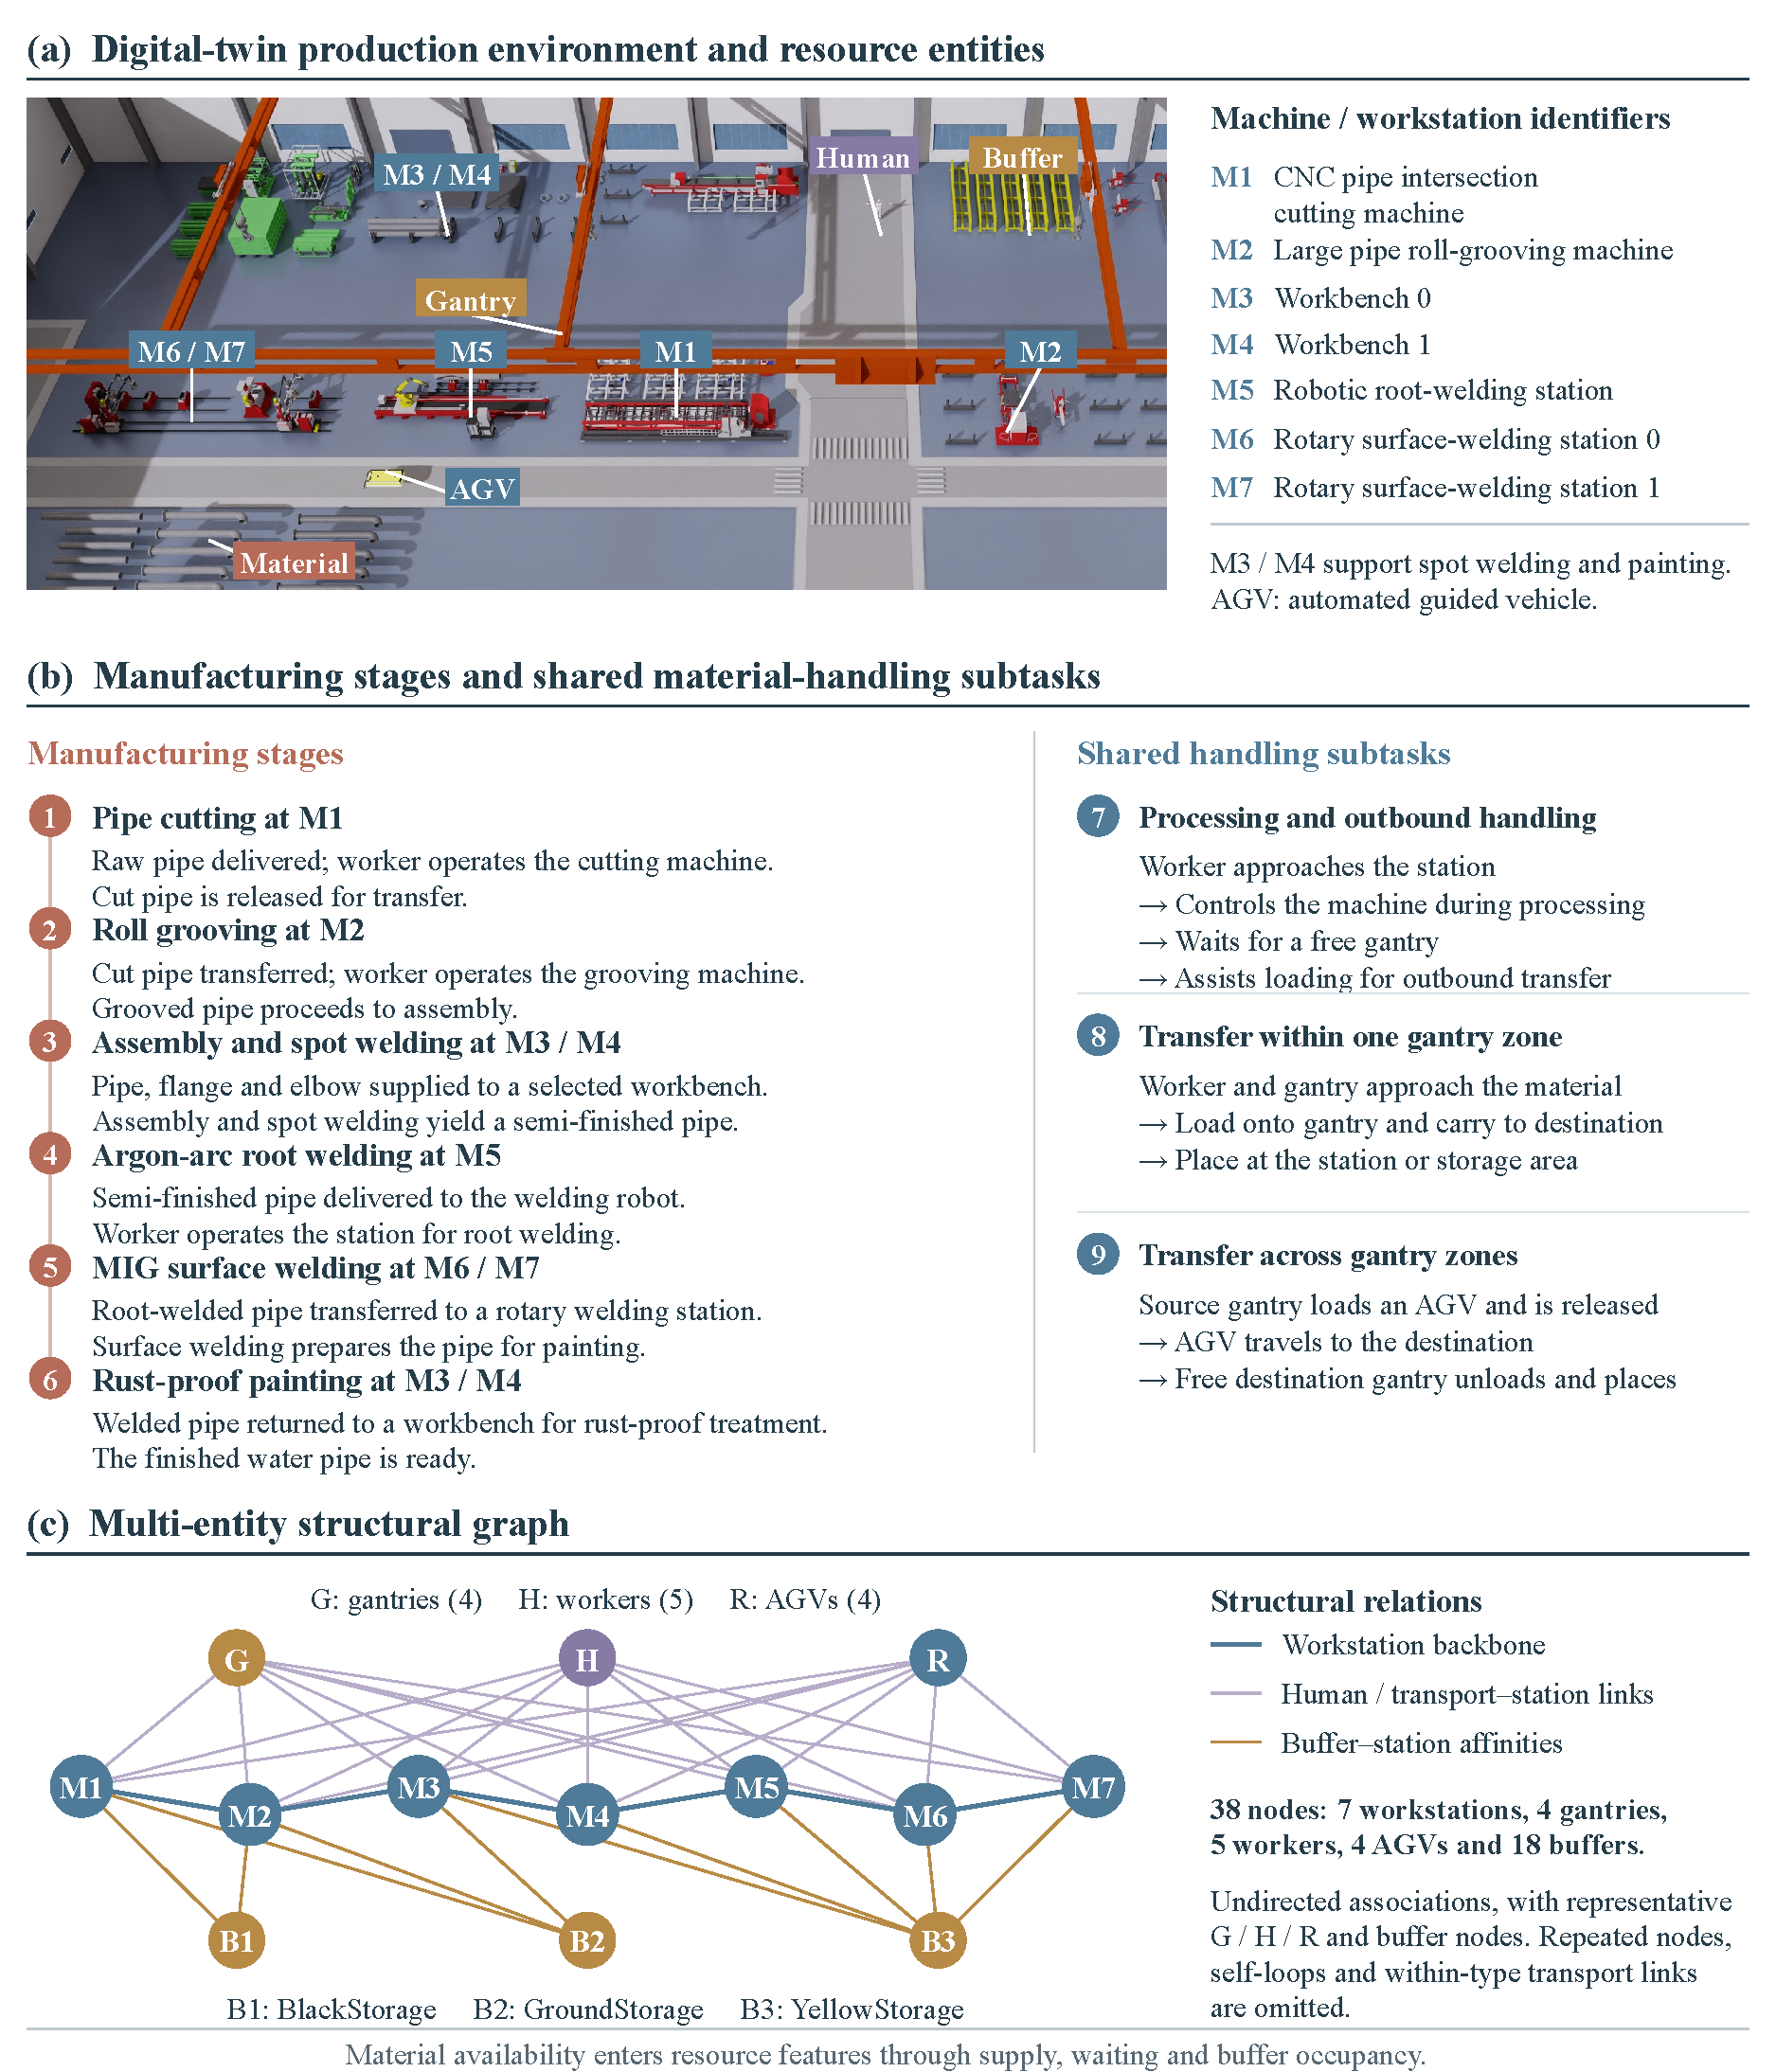
\includegraphics[width=\textwidth]{figures/fig_experiment.pdf}
\caption{Open-workspace factory model developed for NVIDIA Isaac Sim: (a)~resource entities; (b)~manufacturing stages; (c)~structural graph of 38 resources.}
\label{fig:experiment}
\end{figure*}

The data-generation environment exposes four operating variation dimensions and applies each dimension at three intervention levels (Table~\ref{tab:disturbance-design}). Level~0 changes episode-wide resource capacity before each model run, Level~1 perturbs sampled processing or service behaviour, and Level~2 injects temporary events during production. The platform supports intensity $I\in\{1,2,3\}$; slash-separated values in the table follow this order. The formal \texttt{dense\_i1} collection activates one dimension at a time at $I=1$, while nominal runs keep all dimensions inactive. The injected dimension controls data generation but is not used as the bottleneck or process-cause label.

\begin{table*}[t]
\centering
\caption{Four operating variation dimensions and their three intervention levels. Values separated by slashes correspond to $I=1/2/3$. One model step equals one logical second.}
\label{tab:disturbance-design}
\scriptsize
\setlength{\tabcolsep}{3.2pt}
\renewcommand{\arraystretch}{1.12}
\begin{tabularx}{\FullWidth}{@{}lXXX@{}}
\toprule
Dimension & L0: episode configuration & L1: sampled process variation & L2: temporary runtime events \\
\midrule
workstation & Disable workbench ws1 and rotary-welding ws1 & Processing-time noise $5/10/15$ steps; success rate $0.88/0.76/0.64$; tool wear $15/30/45$ steps per 1,000 steps & $2/(2$--$3)/(3$--$4)$ idle-station failures; additional $1$--$2/2$--$3/3$--$4$ weld or kitting quality-hold windows \\
Worker & Reduce workers from 5 to $3/2/1$ & Service-time scale $1.55/2.10/2.65$; worker-specific skill range $0.8$--$1.4/0.7$--$1.6/0.6$--$1.8$; time noise $12/22/32$ steps & $2/(2$--$3)/(3$--$4)$ temporary absences, applied only when the selected worker is idle \\
Logistics & Reduce AGVs from 4 to $2/1/1$; retain all four zone gantries & Gantry-time scale $1.65/2.30/2.95$ with motion noise $10/18/26$ steps; weak background process variation & $2/(2$--$3)/(3$--$4)$ gantry or AGV freezes; at least one pulse targets an AGV while other vehicles remain active \\
Material & Keep the nominal inventory of ten pipes, flanges, and elbows; no permanent deletion & At steps 400--1,000, temporarily hide $6$--$7/7$--$8/7$--$8$ idle flanges or elbows for $1{,}400$--$2{,}200/2{,}000$--$2{,}700/2{,}500$--$3{,}200$ steps & After the opening shortage, inject $1$--$2/2$--$3/3$--$4$ complementary flange/elbow shortage pulses; pipe blanks are never hidden \\
\bottomrule
\end{tabularx}
\end{table*}

For workstation, worker, and logistics operating variations, every Level~2 pulse lasts at least 600 steps and the intensity-specific upper bounds are 900/1,300/1,400 steps. Event targets, start times, counts, and durations are resampled for each episode using a deterministic seed. Adjacent pulses are separated by at least 360 steps, and an event waits for an eligible idle target rather than interrupting an active operation. These controls make the injected condition long enough to survive the eight-window persistence filter while avoiding a deterministic one-to-one mapping between an injection and a labelled bottleneck.

Raw records use logical model time at one-second resolution and include resource-state transitions, workpiece routes and completion times, buffer changes, transport tasks, material inventories, and operating variation logs. The aggregation pipeline reconstructs resource-state intervals and aligns them into non-overlapping 60-s windows. Processing, blockage, starvation, and stoppage durations are accumulated over their overlap with each window; active and unavailable ratios divide the corresponding durations by the window length. Queue features count waiting jobs and summarize their waiting times, while buffer occupancy is averaged over recorded values in the window (carrying forward the preceding value when no update is recorded) and its growth is computed from the difference between the window-end and window-start counts. Process and transport relations supply upstream/downstream state ratios, route delay, inbound waiting, and material-shortage propagation.

All windows share a fixed resource ordering. Each node has 21 operational channels, a five-dimensional resource-type encoding, and one labour-saturation channel, forming a $38\times27$ feature matrix per window. The export routine fills absent numeric entries with zero and recomputes labour saturation from worker activity. Each valid episode ends after all ten workpieces have completed. Runs affected by the known model deadlock defect are discarded as invalid records rather than interpreted as observations of a production operating variation. A run-stratified, episode-level split gives 140/28/36 training/validation/test episodes from 204 valid episodes. Sliding samples use 30 historical windows and a 30-window future grid, with a one-window stride and no crossing of episode boundaries. The resulting partitions contain 20,826/4,331/5,354 forecast windows (Table~\ref{tab:exp-dataset}); feature standardization is fitted on the training histories and applied unchanged to validation and test inputs. All main baseline comparisons use a unified re-evaluation on the same 5,354 shared test-window identities rather than scores from an earlier sample set. Table~\ref{tab:dataset-labels} reports the Upcoming, Ongoing, and no-event composition of the test window--resource pairs under each Start cap.

Operational-state rules combine processing activity, queue buildup, starvation, and resource-coupling indicators into resource-level bottleneck labels. Process-cause targets are derived from the corresponding operating evidence; the report uses material shortage, transport delay, queue buildup, and downstream blockage. Workpiece completion records provide the order-level target: the time from the forecast origin until all ten workpieces have finished.

Process-informed labels apply an eight-window persistence rule (Min8) to newly forming bottlenecks. An event already active at the last historical window is retained when at least one labelled future window remains. We evaluate three onset-cap settings, Start$\leq5$, Start$\leq10$, and Start$\leq15$, which define the admissible distance between the current window and a future event onset. The future grid and the onset cap are kept fixed within each task. A three-window start tolerance is used for strict report matching, and every window corresponds to 60~s; duration, start, and remaining-time errors are consequently reported in minutes.

\begin{table}[pos=t]
\centering
\caption{Dataset and label protocol used in the experiments.}
\label{tab:exp-dataset}
\scriptsize
\setlength{\tabcolsep}{4pt}
\renewcommand{\arraystretch}{1.08}
\begin{tabularx}{\columnwidth}{@{}lX@{}}
\toprule
Item & Setting \\
\midrule
Dataset & \texttt{dense\_i1}, 204 valid episodes, 38 resources \\
Split & 140/28/36 episodes; 20,826/4,331/5,354 windows \\
Windowing & 60-s windows; 30 historical + 30 future windows \\
Targets & 15 resources: 7 workstations, 4 gantries, 4 robots \\
Event rule & Min8 persistence; Start$\leq5/10/15$ \\
Report matching & Three-window onset tolerance \\
\bottomrule
\end{tabularx}
\end{table}

\begin{table}[pos=t]
\centering
\caption{Test-set label composition under each Start cap. Counts are window--resource pairs over 5,354 windows $\times$ 15 targets ($80{,}310$ pairs); parentheses give the share of all pairs.}
\label{tab:dataset-labels}
\scriptsize
\setlength{\tabcolsep}{3.2pt}
\renewcommand{\arraystretch}{1.08}
\begin{tabular*}{\columnwidth}{@{\extracolsep{\fill}}lrrr@{}}
\toprule
Start cap & Upcoming & Ongoing & No-event \\
\midrule
$\leq5$ & 336 (0.42\%) & 766 (0.95\%) & 79,208 (98.63\%) \\
$\leq10$ & 604 (0.75\%) & 768 (0.96\%) & 78,938 (98.29\%) \\
$\leq15$ & 708 (0.88\%) & 770 (0.96\%) & 78,832 (98.16\%) \\
\bottomrule
\end{tabular*}
\end{table}

\subsubsection{Baseline methods}

Four baselines represent complementary modelling families. XGBoost is a gradient-boosted decision-tree predictor operating on tabular summaries, providing a non-neural reference for nonlinear feature interactions. LSTM is a recurrent predictor that models temporal dependencies in the historical sequence. BTGCN constructs a graph over production tasks and combines graph convolution with a GRU to model relational and temporal information~\cite{yin2025btgcn}. BSTAN uses graph attention with a GRU to learn adaptive neighbour contributions for blockage and starvation related prediction~\cite{lai2023bstan}. All baseline comparisons reported in this paper use a unified re-evaluation on the same 5,354 shared test windows, with identical sample identities, history length, future grid, target resources, and event-label definitions for PHGST-PD and the four baselines. Each baseline retains its corresponding input representation and training procedure.

\begin{table}[pos=t]
\centering
\caption{Baseline models and their roles in the comparison.}
\label{tab:exp-baselines}
\scriptsize
\setlength{\tabcolsep}{4pt}
\renewcommand{\arraystretch}{1.10}
\begin{tabularx}{\columnwidth}{@{}lXX@{}}
\toprule
Model & Core framework & Comparison role \\
\midrule
XGBoost & Gradient-boosted decision trees & Tabular predictor \\
LSTM & Long short-term memory & Recurrent temporal predictor \\
BTGCN & Graph convolution + GRU & Graph-convolutional predictor \\
BSTAN & Graph attention + GRU & Graph-attention predictor \\
\bottomrule
\end{tabularx}
\end{table}

\subsubsection{Overall experimental settings and metrics}

PHGST-PD uses five encoder blocks, an 80-dimensional latent representation, eight-dimensional Laplacian positional encoding, $4/2/2$ temporal/geographic/semantic attention heads, a geographic hop-distance cutoff of 4, five semantic neighbours, and 16 length-three pattern keys. AdamW is used with batch size 16, learning rate $5\times10^{-5}$, weight decay $0.05$, cosine decay to $10^{-6}$, and fourfold positive-window oversampling. Training has two stages. Stage~1 learns the bottleneck and cause heads: it starts from the fixed parameter state reused by every ablation arm, unfreezes the last five encoder blocks, and runs for at most 50 epochs with patience 40. The three onset caps are trained as a curriculum (Start$\leq5\rightarrow$Start$\leq10\rightarrow$Start$\leq15$). A far-onset enhancement doubles the onset loss for events starting more than 5~min ahead, sets the far-onset positive weight to $9/10/11$ for the three caps, and raises the false-alarm penalty (weights $2.5$ and $2.2$ for ordinary and hard false positives). Stage~2 freezes the encoder and every bottleneck and cause head, adds a per-workpiece rate term to the remaining-time head, and fine-tunes only that head for at most 20 epochs with validation loss as the selection criterion. This stage specializes the order-progress forecast while preserving the event and cause outputs. All reported training runs use seed 42; the results are point estimates rather than multi-seed stability estimates. Tables~\ref{tab:shared-training-protocol} and~\ref{tab:model-task-parameters} collect the complete shared protocol and model settings used for the reported Full and ablation comparisons.

The checkpoint and report threshold are selected on the validation split. Candidate thresholds are $\{0.45,\dots,0.90,0.94\}$; selection uses the internal station-identification F1 among candidates satisfying validation report precision $\geq0.80$ and recall $\geq0.70$. This selection score is not reported as a result; the reported event metric is the onset-qualified F1-score defined below. All three onset caps use the selected threshold of $0.94$ for testing.

Metrics follow the three prediction dimensions. The reported bottleneck-event F1-score requires both correct station identification and an onset error within three windows. Upcoming recall uses future-event window--resource pairs whose final historical window is non-bottleneck; Ongoing recall uses pairs with an active final historical window. Start and duration MAE are measured on correctly detected events, while union duration MAE/RMSE includes missed and false events. Next-window and 30-window State F1 describe the predicted occupancy over time, including recovery. Process-cause evaluation uses accuracy and macro recall over the four supported classes. Order-completion evaluation uses remaining-time MAE at the line level.

\begin{table*}[t]
\centering
\caption{Metrics used in the main evaluation and component analyses.}
\label{tab:exp-metrics}
\scriptsize
\setlength{\tabcolsep}{3.5pt}
\renewcommand{\arraystretch}{1.08}
\begin{tabular*}{\FullWidth}{@{\extracolsep{\fill}}lll@{}}
\toprule
Metric group & Metric & Interpretation \\
\midrule
Event & F1-score & Station identification with a three-window onset tolerance \\
Early warning & Upcoming / ongoing recall & Station recall: historically cold / active resources \\
State & State F1 (1-step / horizon) & Bottleneck state accuracy at one step / 30-step horizon \\
Temporal & Start MAE; duration MAE & Localization and duration error on detected events \\
Temporal & Union duration MAE/RMSE & Error including missed and false events \\
Auxiliary & Remaining-time MAE & Global order-progress estimation error \\
Auxiliary & Cause accuracy / macro recall & Four supported process-cause classes \\
\bottomrule
\end{tabular*}
\end{table*}

\subsection{Main and baseline performance comparison}\label{sec:comparison-overview}

The comparison evaluates three complementary capabilities of the production forecast. Bottleneck event and temporal prediction identifies the affected resource and describes when its constraint begins, persists, and ends (Table~\ref{tab:comparison-main}); process-cause prediction supplies an operational interpretation of that constraint (Table~\ref{tab:comparison-state}); and order remaining-time prediction estimates line-level completion progress (Table~\ref{tab:comparison-remain}). Together, these outputs provide resource-level warning with process context and an order-progress estimate. All baseline comparisons in this section use a unified re-evaluation on the same 5,354 shared test windows (and the corresponding window--resource pairs), with identical sample identities, target resources, future grid, and label definitions for PHGST-PD and the four baselines.

\subsubsection{Bottleneck occurrence, onset, end, and duration}\label{sec:comparison-event}

PHGST-PD couples resource identification with the expected bottleneck interval and its evolving occupancy. Table~\ref{tab:comparison-main} evaluates this capability through event P/R/F1, Upcoming/Ongoing recall, onset and duration MAE, and one-step/30-step State F1. Onset and duration jointly specify the reported interval within the 30-min horizon, while the future state sequence describes persistence and recovery. Temporal MAE is evaluated on correctly detected events and is read alongside event recall to characterize both coverage and localization.

PHGST-PD combines broad event coverage with early warning across the three onset caps. F1-score reaches $0.804/0.778/0.768$; the reported differences from the strongest baseline are $10.2/16.7/19.1$ percentage points. Upcoming recall remains $0.542/0.535/0.537$, alongside Ongoing recall of $0.937/0.939/0.930$. These results indicate that PHGST-PD detects upcoming bottlenecks while maintaining coverage of ongoing events.

\begin{table*}[t]
\centering
\caption{Bottleneck event and temporal prediction. Classification scores are percentages; timing MAE is in minutes. Within each Start cap, bold marks the best value and underline marks second-best. All entries use the unified 5,354-window re-evaluation in Section~\ref{sec:comparison-overview}.}
\label{tab:comparison-main}
\scriptsize
\setlength{\tabcolsep}{3.2pt}
\renewcommand{\arraystretch}{1.12}
\begin{tabular*}{\FullWidth}{@{\extracolsep{\fill}}lrrrrrrr@{}}
\toprule
Model & \multicolumn{1}{c}{Event identification $\uparrow$} & \multicolumn{2}{c}{Event recall $\uparrow$} & \multicolumn{2}{c}{Timing MAE $\downarrow$} & \multicolumn{2}{c}{State F1 $\uparrow$} \\
\cmidrule(lr){2-2}\cmidrule(lr){3-4}\cmidrule(lr){5-6}\cmidrule(l){7-8}
 & F1-score & Upcoming & Ongoing & Start & Duration & 1 step & 30 steps \\
\midrule
\multicolumn{8}{l}{\textit{Start $\leq5$}} \\
PHGST-PD & \textbf{80.4\%} & \textbf{54.2\%} & \textbf{93.7\%} & 0.127 & \textbf{1.863} & \textbf{88.3\%} & \textbf{52.5\%} \\
XGBoost & \underline{70.2\%} & 6.0\% & \underline{81.9\%} & \underline{0.030} & \underline{3.264} & 61.1\% & 37.3\% \\
LSTM & 58.3\% & \underline{9.9\%} & 68.7\% & 0.056 & 3.855 & 29.5\% & 29.5\% \\
BTGCN & 66.9\% & 4.6\% & 78.6\% & \textbf{0.020} & 3.322 & 64.3\% & 37.2\% \\
BSTAN & 68.7\% & 9.5\% & 79.4\% & 0.043 & 3.565 & \underline{71.9\%} & \underline{37.9\%} \\
\midrule
\multicolumn{8}{l}{\textit{Start $\leq10$}} \\
PHGST-PD & \textbf{77.8\%} & \textbf{53.5\%} & \textbf{93.9\%} & 0.227 & \textbf{1.788} & \textbf{89.2\%} & \textbf{58.9\%} \\
XGBoost & \underline{61.1\%} & 4.1\% & \underline{80.5\%} & \underline{0.122} & \underline{3.210} & 59.5\% & 33.7\% \\
LSTM & 47.7\% & \underline{11.2\%} & 69.3\% & 0.388 & 3.768 & 27.5\% & 26.2\% \\
BTGCN & 57.9\% & 4.5\% & 72.2\% & \textbf{0.117} & 3.238 & 56.6\% & 35.9\% \\
BSTAN & 60.9\% & 5.7\% & 79.6\% & 0.153 & 3.533 & \underline{63.2\%} & \underline{36.5\%} \\
\midrule
\multicolumn{8}{l}{\textit{Start $\leq15$}} \\
PHGST-PD & \textbf{76.8\%} & \textbf{53.7\%} & \textbf{93.0\%} & 0.227 & \textbf{1.716} & \textbf{90.0\%} & \textbf{61.0\%} \\
XGBoost & \underline{57.7\%} & 3.9\% & \underline{79.6\%} & \textbf{0.167} & 3.170 & 58.2\% & 32.2\% \\
LSTM & 46.1\% & \underline{10.2\%} & 64.3\% & 0.453 & 3.615 & 26.8\% & 26.0\% \\
BTGCN & 51.8\% & 5.4\% & 69.9\% & 0.302 & \underline{3.121} & 46.1\% & 32.3\% \\
BSTAN & 53.4\% & 4.4\% & 70.0\% & \underline{0.222} & 3.422 & \underline{59.3\%} & \underline{33.5\%} \\
\bottomrule
\end{tabular*}
\end{table*}

The temporal outputs extend event identification into a forecast of how long a resource will remain constrained. PHGST-PD's onset MAE is $0.127/0.227/0.227$~min, and detected-event duration MAE is $1.863/1.788/1.716$~min. The latter corresponds to reductions of $42.9\%/44.3\%/45.0\%$ relative to the lowest reported baseline errors. One-step State F1 reaches $0.883/0.892/0.900$, and 30-step State F1 reaches $0.525/0.589/0.610$, exceeding the strongest reported baseline by $14.6/22.4/27.5$ percentage points at the full horizon. Together, the onset, duration, and occupancy predictions describe when a resource is expected to become constrained and recover, providing temporal context for intervention planning. Figure~\ref{fig:baseline-comparison} summarizes F1-score, Upcoming recall, and duration MAE: PHGST-PD maintains Upcoming recall near $0.54$ and duration MAE below 2~min across all three cap settings.

\begin{figure*}[t]
\centering
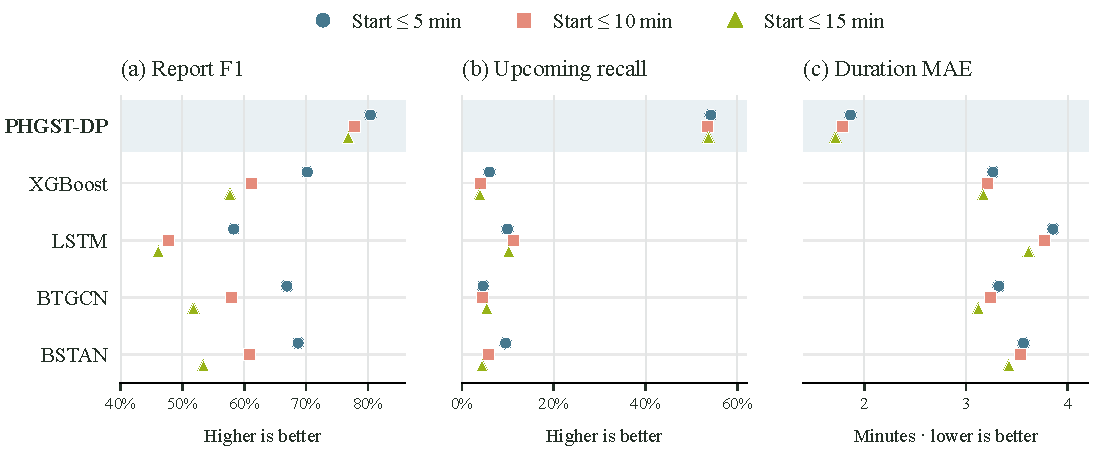
\includegraphics[width=0.96\textwidth]{figures/fig_range_response.pdf}
\caption{Grouped comparison of (a)~F1-score, (b)~Upcoming recall, and (c)~detected-event duration MAE across Start caps.}
\label{fig:baseline-comparison}
\end{figure*}

Within the Start$\leq15$ task, grouping events by their true onset distance shows how warning extends into the future: strict report recall is $0.574$, $0.522$, and $0.433$ for onsets within 5, 6--10, and more than 10~min, respectively. The last group directly demonstrates warning coverage beyond 10~min. Across the three separately configured cap tasks, exact-onset accuracy among station-matched true positives is $0.896/0.844/0.831$, and onset-bucket accuracy is $0.921/0.918/0.920$. Warning also spans processing and material handling: workstation/gantry/robot F1 is $0.805/0.811/0.771$ at Start$\leq5$ and $0.751/0.840/0.639$ at Start$\leq15$. These results place the temporal forecast across the resource types through which production constraints emerge.

\subsubsection{Bottleneck process-cause prediction}\label{sec:comparison-cause}

PHGST-PD predicts process causes alongside its event and temporal forecasts, with cause accuracy of $0.965/0.962/0.974$ and macro recall of $0.967/0.965/0.978$ across the three caps (Table~\ref{tab:comparison-state}). XGBoost records the highest values, with accuracy of $0.990$ and macro recall of $0.988$ under each cap. PHGST-PD ranks second, trailing XGBoost by $1.6$--$2.8$ percentage points in accuracy and $1.0$--$2.3$ points in macro recall. It outperforms the three neural baselines on both metrics under every cap. Its cause classification output complements event coverage by providing graph-level process context in the categories of material shortage, transport delay, queue buildup, and downstream blockage.

\begin{table*}[t]
\centering
\caption{Bottleneck process-cause prediction (\%). Each Start-cap group reports accuracy and macro recall. Within each Start-cap metric, bold marks the best value and underline marks second-best among the compared models. All entries use the unified 5,354-window re-evaluation in Section~\ref{sec:comparison-overview}.}
\label{tab:comparison-state}
\scriptsize
\setlength{\tabcolsep}{3.2pt}
\renewcommand{\arraystretch}{1.12}
\begin{tabular*}{\FullWidth}{@{\extracolsep{\fill}}lrrrrrr@{}}
\toprule
Model & \multicolumn{2}{c}{Start $\leq5$} & \multicolumn{2}{c}{Start $\leq10$} & \multicolumn{2}{c}{Start $\leq15$} \\
\cmidrule(lr){2-3}\cmidrule(lr){4-5}\cmidrule(l){6-7}
 & Accuracy $\uparrow$ & Macro R $\uparrow$ & Accuracy $\uparrow$ & Macro R $\uparrow$ & Accuracy $\uparrow$ & Macro R $\uparrow$ \\
\midrule
PHGST-PD & \underline{96.5\%} & \underline{96.7\%} & \underline{96.2\%} & \underline{96.5\%} & \underline{97.4\%} & \underline{97.8\%} \\
XGBoost & \textbf{99.0\%} & \textbf{98.8\%} & \textbf{99.0\%} & \textbf{98.8\%} & \textbf{99.0\%} & \textbf{98.8\%} \\
LSTM & 93.8\% & 92.0\% & 93.6\% & 93.0\% & 94.4\% & 92.2\% \\
BTGCN & 90.0\% & 88.2\% & 90.7\% & 90.0\% & 90.7\% & 90.0\% \\
BSTAN & 95.7\% & 95.2\% & 95.9\% & 95.1\% & 95.1\% & 93.5\% \\
\bottomrule
\end{tabular*}
\end{table*}


\subsubsection{Order-completion remaining-time prediction}\label{sec:comparison-remain}

Order remaining time is a line-level scalar target that complements resource-level bottleneck forecasts. Table~\ref{tab:comparison-remain} reports global remaining-time MAE under the same unified 5,354-window re-evaluation used for the event and cause comparisons. XGBoost records the lowest MAE, $5.23$~min under each Start cap, whereas PHGST-PD after stage-2 fine-tuning records $9.60/9.27/8.91$~min at Start$\leq5/10/15$. Under this common-sample protocol, XGBoost is the more accurate order remaining-time predictor among the compared models.

\begin{table}[pos=htbp]
\centering
\caption{Global order remaining-time MAE (min; lower is better). Within each Start cap, bold marks the best value and underline marks second-best. All entries use the unified 5,354-window re-evaluation in Section~\ref{sec:comparison-overview}.}
\label{tab:comparison-remain}
\scriptsize
\setlength{\tabcolsep}{3pt}
\renewcommand{\arraystretch}{1.10}
\begin{tabular*}{\columnwidth}{@{\extracolsep{\fill}}lrrr@{}}
\toprule
Model & Start $\leq5$ & Start $\leq10$ & Start $\leq15$ \\
\midrule
XGBoost & \textbf{5.23} & \textbf{5.23} & \textbf{5.23} \\
LSTM & 10.59 & 10.61 & 9.01 \\
BTGCN & 19.34 & 18.10 & 12.83 \\
BSTAN & 14.70 & 13.85 & 13.56 \\
\midrule
PHGST-PD (stage 1) & 10.93 & 11.21 & 9.72 \\
PHGST-PD (stage 2) & \underline{9.60} & \underline{9.27} & \underline{8.91} \\
\bottomrule
\end{tabular*}
\end{table}

A possible explanation concerns the representation and optimization used for this target. In the baseline design, XGBoost trains an independent remaining-time regressor using recent historical statistics, global state, and explicit order-progress features, including remaining workpiece count, total count, and remaining fraction. Its piecewise nonlinear regression may be well suited to progress--completion-time relationships. PHGST-PD first learns a shared representation for bottleneck events and their temporal and process context; stage~2 freezes the encoder and event and cause heads while optimizing the remaining-time head. PHGST-PD also conditions this head on the remaining workpiece fraction and total count, and its stage-2 rate term uses the remaining count. Thus, the observed gap cannot be attributed simply to an absence of progress information in PHGST-PD. The common-sample results are consistent with the interpretation that independently optimized tree regression fits this order-level target better than the frozen shared representation under the evaluated configuration.

Stage-2 fine-tuning reduces PHGST-PD MAE from $10.93/11.21/9.72$ to $9.60/9.27/8.91$~min while retaining the event and cause outputs (Figure~\ref{fig:remain-finetune}). This improvement supports the value of task-specific optimization, but does not establish superiority over a dedicated regressor. PHGST-PD's contribution is to report order progress together with resource-level advance warning and process explanations.

\subsection{Ablation study}

The ablation study links predictive performance to three design choices: heterogeneous process--logistics information, process-informed supervision and temporal pattern clustering, and the propagation-delay-aware module. Nine configurations also examine the decoder and training choices that support advance warning (Table~\ref{tab:ablation-arms}). Every ablation comparison, including its Full reference, is evaluated on the same 5,354 shared test windows used in Section~\ref{sec:comparison-overview}, begins from identical parameter values, and uses a 50-epoch budget, the same Start$\leq5\rightarrow$Start$\leq10\rightarrow$Start$\leq15$ curriculum, and the same validation-controlled checkpoint and threshold-selection rule. Dataset, target resources, label rules, and candidate thresholds also follow the same protocol. The common selection procedure yields a threshold of $0.94$ for most arms and $0.90/0.88/0.94$ for NoFarBoost. The matched-budget cause-supervision experiment separately isolates the explanatory effect of the cause head. Remaining-time comparisons within the ablation study use the stage-1 reference, before head-specific fine-tuning.

\begin{table*}[t]
\centering
\caption{Ablation arms. Every comparison, including the Full reference, begins from identical parameter values and uses the same 50-epoch budget, Start$\leq5\rightarrow$Start$\leq10\rightarrow$Start$\leq15$ curriculum, and validation-controlled model-selection rule.}
\label{tab:ablation-arms}
\scriptsize
\setlength{\tabcolsep}{3.5pt}
\renewcommand{\arraystretch}{1.08}
\begin{tabular*}{\FullWidth}{@{\extracolsep{\fill}}llll@{}}
\toprule
Arm & Contribution & Change relative to the retained model & Training \\
\midrule
NoGraph & Heterogeneous graph & Self-loop adjacency only; no factory edges & Common protocol, 50 ep. \\
NoGroup & Heterogeneous graph & One linear projection of the 27 channels instead of six semantic groups & Common protocol, 50 ep. \\
NoCross & Heterogeneous graph & Within-type edges only; cross-type semantic attention masked & Common protocol, 50 ep. \\
NoInfo & Heterogeneous graph & Only workstations observed; non-workstation features and five coupling channels zeroed & Common protocol, 50 ep. \\
WorkstationOnly & Heterogeneous graph & NoCross and NoInfo combined & Common protocol, 50 ep. \\
NoCluster & Temporal pattern clustering & Temporal pattern clustering removed & Common protocol, 50 ep. \\
NoPattern & \makecell[l]{Propagation-delay-aware module} & Recent-patch matching to the temporal-pattern prototype bank disabled & Common protocol, 50 ep. \\
NoSplit & Decoder & One shared will head for continuing and new events & Common protocol, 50 ep. \\
NoFarBoost & Training & Far-onset weighting and enhanced false-alarm penalty removed & Common protocol, 50 ep. \\
\bottomrule
\end{tabular*}
\end{table*}

PHGST-PD preserves event accuracy as the onset range expands (Table~\ref{tab:ablation-grouped}). Most removed components lower F1-score and Upcoming recall and raise union duration error, while NoFarBoost is slightly better at Start$\leq5$ at its validation-selected threshold. From Start$\leq5$ to Start$\leq15$, Full F1-score changes from $0.804$ to $0.768$, and union duration MAE from $4.17$ to $4.43$~min. Under the matched initialization, budget, curriculum, and model-selection protocol, the structural and entity variants exhibit larger changes, with F1 reductions of approximately $0.052$--$0.328$ and union duration MAE increases of $0.95$--$3.23$~min across NoGraph, NoGroup, NoCross, NoInfo, and WorkstationOnly over the three onset caps. For the propagation-delay-aware module, Upcoming recall holds with Full across caps, whereas NoPattern and NoSplit degrade more sharply, and the $>10$~min strict-report bin rises from $0.240$ (NoFarBoost) to $0.433$ (Full).

\subsubsection{Heterogeneous graph and multi-entity information}

This experiment examines the value of observing multiple resource entities and exchanging information across their process relations (Table~\ref{tab:entity-ablation-new}). NoGraph and NoGroup remove the factory graph and grouped embedding, respectively. NoCross retains all observations and restricts interaction to the same resource type. NoInfo uses workstation observations with five coupling channels masked: route delay, inbound waiting, shortage propagation, blocked-minus-starved time, and labour saturation. WorkstationOnly combines the NoCross and NoInfo restrictions.

\begin{table*}[t]
\centering
\caption{Ablation of the heterogeneous graph, grouped embedding, and multi-entity information. Type hmean is the harmonic mean of workstation, gantry, and AGV occupancy F1; Dur.\ MAE is the union duration MAE (min; lower is better). Within each Start cap, bold marks the best value and underline marks second-best. NoInfo and WorkstationOnly retain the same evaluation targets; their zero type hmean reflects zero occupancy F1 for at least one resource type after the associated input information is removed.}
\label{tab:entity-ablation-new}
\scriptsize
\setlength{\tabcolsep}{3.5pt}
\renewcommand{\arraystretch}{1.05}
\begin{tabular*}{\FullWidth}{@{\extracolsep{\fill}}llrrrrr@{}}
\toprule
Arm & Start cap & F1-score & Upcoming R & Type hmean & State F1 (1-step) & Dur.\ MAE \\
\midrule
Full & $\leq5$ & \textbf{80.4\%} & \textbf{54.2\%} & \textbf{50.5\%} & \textbf{88.3\%} & \textbf{4.17} \\
NoGraph &  & 74.6\% & 10.4\% & 38.4\% & \underline{87.3\%} & 5.48 \\
NoGroup &  & \underline{75.3\%} & \underline{33.3\%} & \underline{43.2\%} & 83.5\% & \underline{5.11} \\
NoCross &  & 71.6\% & 22.0\% & 39.6\% & 81.2\% & 5.28 \\
NoInfo &  & 64.4\% & 4.9\% & 0.0\% & 69.9\% & 6.66 \\
WorkstationOnly &  & 65.0\% & 3.3\% & 0.0\% & 70.9\% & 6.51 \\
\midrule
Full & $\leq10$ & \textbf{77.8\%} & \textbf{53.5\%} & \textbf{53.0\%} & \textbf{89.2\%} & \textbf{4.38} \\
NoGraph &  & 64.9\% & 6.5\% & 37.6\% & \underline{84.4\%} & 6.46 \\
NoGroup &  & \underline{65.1\%} & \underline{48.5\%} & \underline{45.2\%} & 82.6\% & \underline{6.05} \\
NoCross &  & 57.1\% & 20.7\% & 37.1\% & 75.9\% & 6.60 \\
NoInfo &  & 54.4\% & 2.1\% & 0.0\% & 68.4\% & 7.57 \\
WorkstationOnly &  & 55.9\% & 1.4\% & 0.0\% & 70.8\% & 7.40 \\
\midrule
Full & $\leq15$ & \textbf{76.8\%} & \textbf{53.7\%} & \textbf{53.6\%} & \textbf{90.0\%} & \textbf{4.43} \\
NoGraph &  & \underline{61.2\%} & 3.7\% & 36.0\% & \underline{86.5\%} & 6.57 \\
NoGroup &  & 60.4\% & \underline{43.2\%} & \underline{46.9\%} & 81.9\% & \underline{6.34} \\
NoCross &  & 51.4\% & 31.1\% & 36.5\% & 76.0\% & 6.77 \\
NoInfo &  & 44.1\% & 21.8\% & 0.0\% & 59.6\% & 7.66 \\
WorkstationOnly &  & 53.4\% & 2.1\% & 0.0\% & 70.6\% & 7.46 \\
\bottomrule
\end{tabular*}
\end{table*}

Cross-resource information is most closely associated with advance warning. PHGST-PD's Upcoming recall is $0.542/0.535/0.537$, compared with $0.049/0.021/0.218$ for NoInfo and $0.033/0.014/0.021$ for WorkstationOnly. At Start$\leq15$, strict report recall for events beginning more than 10~min ahead is $0.433$ for Full, compared with $0.192$ for NoGroup, $0.067$ for NoCross, and $0$ for NoGraph (Figure~\ref{fig:cross-resource-evidence}a). The resource-type hmean remains $0.505$--$0.536$ for Full but falls to $0.360$--$0.384$ for NoGraph and $0.365$--$0.396$ for NoCross across the three caps (Figure~\ref{fig:cross-resource-evidence}b). Together, the two views associate cross-resource structure with both distant-event coverage and balanced performance across workstation, gantry, and AGV targets. The device traces in Figure~\ref{fig:key-device-entity} connect these aggregate differences to event persistence: PHGST-PD identifies both intervals about 5~min before NoInfo and WorkstationOnly, whose duration estimates remain at 6--8~min during the displayed 20-min reference plateau; NoCross reaches 14~min before decaying to about 8~min.

\begin{figure}[pos=htbp]
\centering
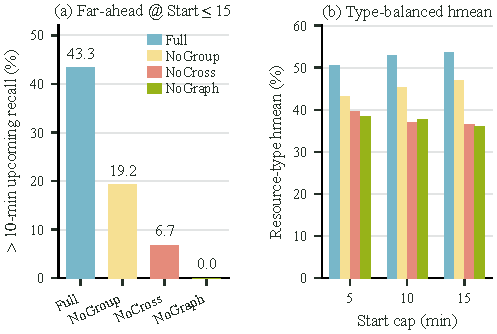
\includegraphics[width=\columnwidth]{figures/fig_cross_resource_evidence.pdf}
\caption{Cross-resource evidence from structural ablations: (a)~far-onset report recall at Start$\leq15$; (b)~type-hmean F1 across Start caps.}
\label{fig:cross-resource-evidence}
\end{figure}

\begin{figure*}[t]
\centering
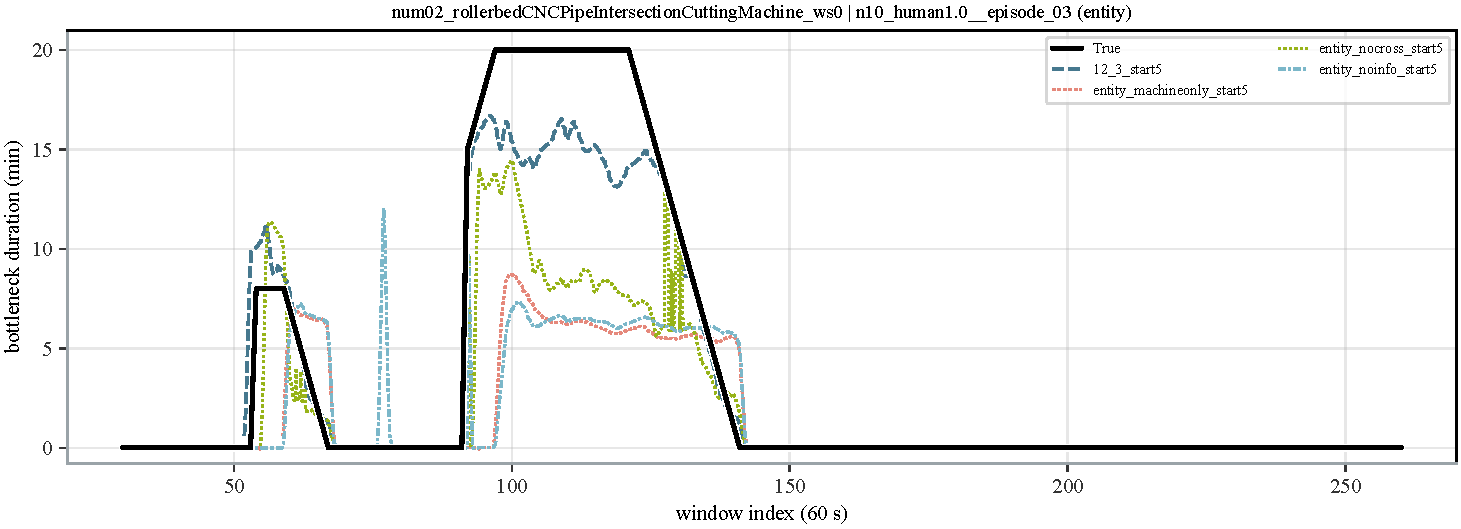
\includegraphics[width=0.96\textwidth]{figures/key_device_entity.pdf}
\caption{Key-device duration traces: (a)~multi-entity ablations at Start$\leq5$; (b)~PHGST-PD under Start$\leq5/10/15$ on the same episode.}
\label{fig:key-device-entity}
\end{figure*}

\paragraph*{Learned cross-resource allocation under mixed operating conditions.}
Attention sampling and averaging follow the protocol in Section~\ref{sec:attention-protocol}. Figure~\ref{fig:attn-change} retains the resource-level change maps underlying the main-text type summary.

Upcoming and ongoing averages are compared with normal attention. Colour indicates increased or decreased weight; the absolute reference matrices are retained below.

\begin{figure*}[pos=!htbp]
\centering
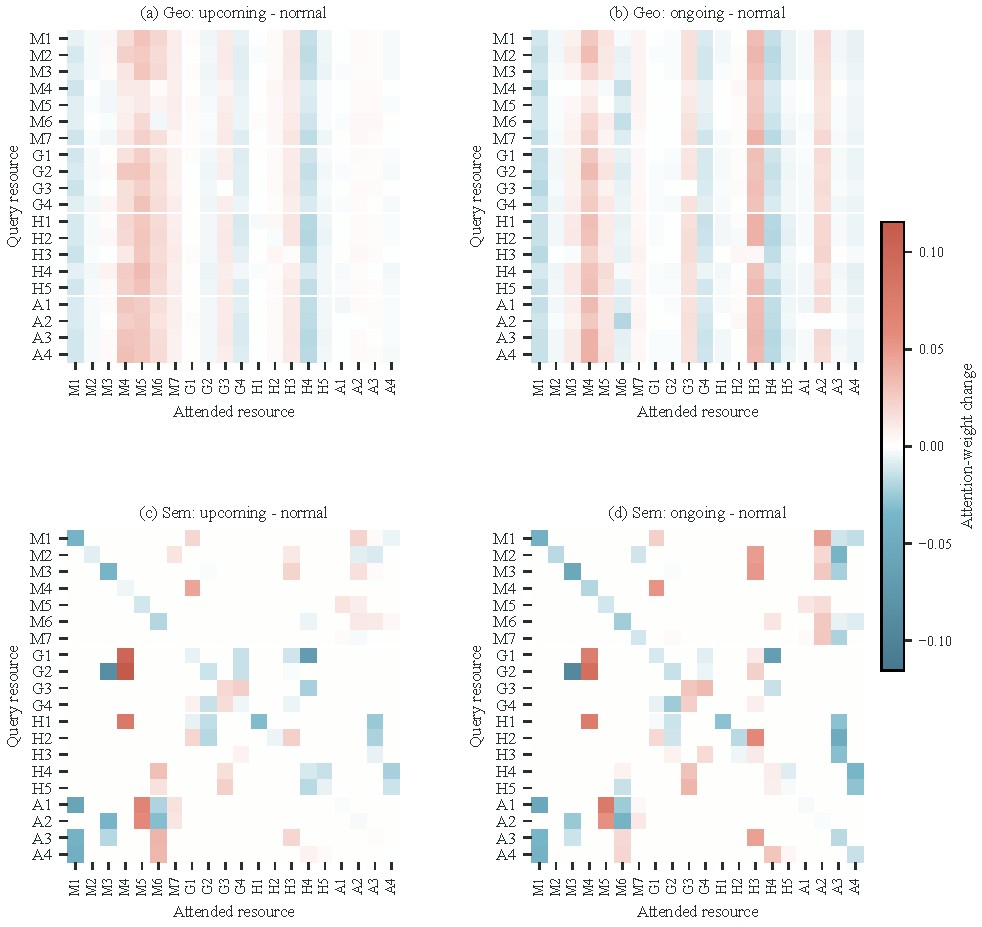
\includegraphics[width=0.92\textwidth]{figures/attention_heatmaps/fig03_resource_attention_change.pdf}
\caption{Resource-attention redistribution relative to normal for upcoming and ongoing samples (coral: increase; blue: decrease).}
\label{fig:attn-change}
\end{figure*}



\subsubsection{Process-informed supervision and temporal pattern clustering}\label{sec:supervision-analysis}
% Prefer text+float sharing a column page; avoid near-empty float pages.
\setcounter{topnumber}{3}
\setcounter{bottomnumber}{2}
\setcounter{totalnumber}{5}
\renewcommand{\topfraction}{0.9}
\renewcommand{\bottomfraction}{0.8}
\renewcommand{\textfraction}{0.15}
\renewcommand{\floatpagefraction}{0.75}
\renewcommand{\dbltopfraction}{0.9}

Process-informed supervision connects the event representation to production meaning. The analysis focuses on temporal pattern clustering, cause accuracy under a matched training budget, and alignment between process-informed label rankings and intervention-sensitive resources. These experiments answer different questions and are therefore interpreted separately.

\paragraph*{(1) Effects of temporal pattern clustering.}
NoCluster removes temporal pattern clustering to assess its contribution to recurrent temporal-pattern prototype construction. NoPattern separately disables the use of prototype matching in the propagation-delay-aware module.

\begin{table*}[t]
\centering
\caption{Event, state, and duration metrics for the Full configuration and NoCluster (temporal pattern clustering removed). Dur.\ MAE is the union error (min); Dur.\ MAE (tp) is computed on correctly reported events only.}
\label{tab:group-ablation}
\scriptsize
\setlength{\tabcolsep}{3.5pt}
\renewcommand{\arraystretch}{1.08}
\begin{tabular*}{\FullWidth}{@{\extracolsep{\fill}}llrrrrr@{}}
\toprule
Arm & Start cap & F1-score & Upcoming R & State F1 (1-step) & Dur.\ MAE & Dur.\ MAE (tp) \\
\midrule
Full & $\leq5$ & \textbf{80.4\%} & \textbf{54.2\%} & \textbf{88.3\%} & \textbf{4.17} & \textbf{1.86} \\
NoCluster & & 73.4\% & 12.5\% & 84.1\% & 5.43 & 2.89 \\
\midrule
Full & $\leq10$ & \textbf{77.8\%} & \textbf{53.5\%} & \textbf{89.2\%} & \textbf{4.38} & \textbf{1.79} \\
NoCluster & & 57.0\% & 34.6\% & 78.9\% & 6.69 & 2.40 \\
\midrule
Full & $\leq15$ & \textbf{76.8\%} & \textbf{53.7\%} & \textbf{90.0\%} & \textbf{4.43} & \textbf{1.72} \\
NoCluster & & 53.7\% & 37.3\% & 81.9\% & 6.65 & 2.30 \\
\bottomrule
\end{tabular*}
\end{table*}

\paragraph*{(2) Effects of cause supervision.}
Cause supervision improves prediction of the rule-derived process-cause labels under matched training conditions (Table~\ref{tab:matched-cause}). With PHGST-PD labels, a common data split, Start$\leq5$, seed 42, random initialization, and a 50-epoch budget, logged cause accuracy rises from $19.5\%$ to $89.5\%$, and the separately selected cause accuracy and macro recall rise from $25.2\%/25.5\%$ to $92.2\%/93.7\%$. Logged station F1 remains near $73\%$, so the measured benefit is localized to the explanatory output.

\begin{table}[pos=htbp]
\centering
\caption{Matched-budget cause-supervision study at Start$\leq5$ (seed 42; 50 epochs). Values are percentages. Logged metrics come from the training export; selected cause metrics use a separately chosen operating point and are not interchanged with the logged values.}
\label{tab:matched-cause}
\scriptsize
\setlength{\tabcolsep}{3.5pt}
\renewcommand{\arraystretch}{1.08}
\begin{tabular*}{\columnwidth}{@{\extracolsep{\fill}}lrr@{}}
\toprule
Metric & Backbone & +Cause \\
\midrule
Logged station F1 & 73.5\% & 73.3\% \\
Logged cause acc. & 19.5\% & \textbf{89.5\%} \\
Selected cause acc. & 25.2\% & \textbf{92.2\%} \\
Selected cause macro recall & 25.5\% & \textbf{93.7\%} \\
\bottomrule
\end{tabular*}
\end{table}

% Evidence: isaac_factory origin/dev_tyx, 8767583f3ed6392cfd8061d4a80de94fcfb9d7a0.
% Source: bottleneck ground-truth validity notes (2026-10-14), checked against label/evaluation code.
% Imported summary values: experiments/data/label_validity_dev_tyx_8767583.json.
\paragraph*{(3) Validation against production sensitivity.}
Production sensitivity provides an operational criterion for bottleneck labels: prioritizing resources whose temporary acceleration shortens order completion. Counterfactual replay compares a service intervention with the unchanged production trajectory from the same saved state. This connects the label ranking to the consequence of a resource-level action.

At a saved factory-model state $t$, each of seven workstation candidates receives a separate service-bundle intervention. Workstation processing and its associated worker service use a duration scale of $0.8$, equivalent to a $1.25\times$ service rate, for 1,200 model steps. Baseline and intervention branches start from the same saved state and random-number state and run to order completion. The counterfactual sensitivity is
\begin{equation}
S_i(t)=M_{\mathrm{base}}(t)-M_{i,0.8}(t),
\end{equation}
where $M$ denotes order-completion time. Positive $S_i(t)$ indicates that temporarily accelerating resource $i$ shortens the order. Each label method ranks candidates using its maximum evidence over the last three fully observed windows before $t$.

PHGST-PD yields the highest point estimates on all five sensitivity-alignment metrics in the three-episode nominal-condition pilot (Figure~\ref{fig:label-oracle-pilot}). NDCG@3 measures ranking quality using positive sensitivity as relevance; Positive Recall@$k$ measures coverage of the oracle's $k$ highest positive-sensitivity resources by the first $k$ candidates. Weighted Recall@3 gives the fraction of total positive sensitivity captured by the first three candidates, and Coverage@3$_{0.9}$ covers resources satisfying $S_i\geq0.9\max_j S_j$. PHGST-PD reaches NDCG@3 $0.531$ and Weighted Recall@3 $0.716$, compared with $0.495$ and $0.585$ for Queue-Wait. The mean weighted coverage of positive sensitivity by its top-three candidates is $71.6\%$ under this pilot protocol. Early-, middle-, and late-stage NDCG@3 values are $0.421/0.339/0.770$, with the strongest alignment near order completion.

\begin{figure}[pos=htbp]
\centering
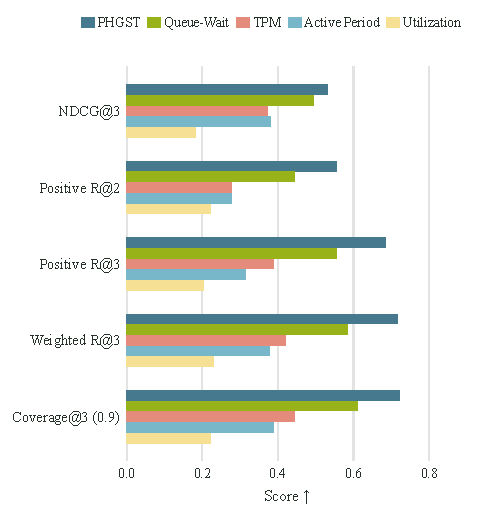
\includegraphics[width=\columnwidth]{figures/fig_label_oracle_bars.pdf}
\caption{Counterfactual sensitivity alignment in the exploratory pilot (↑ better).}
\label{fig:label-oracle-pilot}
\end{figure}

These exploratory estimates support production sensitivity as a distinct dimension of supervision quality. All five retained soft-alignment metrics favour PHGST-PD in this pilot, but the metric set was finalized after inspecting the pilot and Holm-adjusted paired comparisons do not reject the null hypotheses. The independent full-Oracle evaluation has not been run; the numerical ordering is therefore interpreted only as a development result for nominal-condition episodes, not as proof of general superiority across operating conditions.

\subsubsection{Propagation-delay-aware module}

Temporal pattern clustering supplies the recurrent prototype bank, while the propagation-delay-aware module uses that bank to support warnings that precede the visible bottleneck state. PHGST-PD records Upcoming recall of $0.542/0.535/0.537$, compared with $0.167/0.278/0.427$ for NoPattern, which retains the graph and attention branches while disabling the matching of recent patches to the temporal-pattern prototype bank (Table~\ref{tab:delay-ablation-new}). For events starting more than 10~min ahead, strict report recall is $0.433$ versus $0.163$. This distance-resolved result is consistent with the role of prototype-conditioned historical context in representing delayed propagation. Cause macro recall is $0.967/0.965/0.978$ for Full and $0.734/0.805/0.850$ for NoPattern; the largest class-level contrast is queue buildup, with recall $0.984$ versus $0.145$ at Start$\leq5$. The stage-1 remaining-time reference also records MAE $10.93/11.21/9.72$~min, compared with $18.62/13.35/11.06$~min for NoPattern, linking temporal context to order-progress estimation.

\begin{table*}[t]
\centering
\caption{Ablation of temporal-pattern prototype matching in the propagation-delay-aware module. $R_{\mathrm{up,rep}}$ is strict report recall within the stated onset-distance bin; Cause Macro R is macro recall over the four supported process-cause classes. Remain MAE (min) is compared with the stage-1 model, which, like the ablation, has no remaining-time fine-tuning.}
\label{tab:delay-ablation-new}
\scriptsize
\setlength{\tabcolsep}{2.6pt}
\renewcommand{\arraystretch}{1.08}
\begin{tabular*}{\FullWidth}{@{\extracolsep{\fill}}llrrrrrrr@{}}
\toprule
Arm & Start cap & F1-score & Upcoming R & $R_{\mathrm{up,rep}}^{6\text{--}10}$ & $R_{\mathrm{up,rep}}^{>10}$ & Queue R & Cause Macro R & Remain MAE \\
\midrule
Full (stage 1) & $\leq5$ & \textbf{80.4\%} & \textbf{54.2\%} & --- & --- & \textbf{98.4\%} & \textbf{96.7\%} & \textbf{10.93} \\
NoPattern & & 74.5\% & 16.7\% & --- & --- & 14.5\% & 73.4\% & 18.62 \\
\midrule
Full (stage 1) & $\leq10$ & \textbf{77.8\%} & \textbf{53.5\%} & \textbf{46.6\%} & --- & \textbf{98.4\%} & \textbf{96.5\%} & \textbf{11.21} \\
NoPattern & & 58.8\% & 27.8\% & 14.9\% & --- & 47.6\% & 80.5\% & 13.35 \\
\midrule
Full (stage 1) & $\leq15$ & \textbf{76.8\%} & \textbf{53.7\%} & \textbf{52.2\%} & \textbf{43.3\%} & \textbf{98.4\%} & \textbf{97.8\%} & \textbf{9.72} \\
NoPattern & & 60.1\% & 42.7\% & 39.6\% & 16.3\% & 57.3\% & 85.0\% & 11.06 \\
\bottomrule
\end{tabular*}
\end{table*}

\paragraph*{Historical and layer-wise attention structure.}
Figures~\ref{fig:attn-temporal}--\ref{fig:attn-horizons} examine temporal context within the same supplementary mixed-disturbance analysis. Figure~\ref{fig:attn-temporal} covers all 30 historical windows under normal and upcoming conditions, with an upcoming-minus-normal panel that resolves smaller shifts in the historical positions receiving attention. Its difference scale is much narrower than the absolute-weight scale, so the panel should not be read as a large change in temporal dependence. Figure~\ref{fig:attn-layers} focuses the main-text comparison on encoder layers 1, 4, and 5, retaining an input-near layer and the final two layers while keeping both geographic and semantic branches readable. The complete five-layer view is retained in Appendix~\ref{app:layerwise-attention}. Layer-specific weights do not measure the accuracy contribution of each layer.

Figure~\ref{fig:attn-horizons} compares the upcoming-minus-normal resource maps from three separately trained Start$\leq5/10/15$ mixed-disturbance checkpoints, with 96 samples per condition and checkpoint. The persistent structure and localized changes provide a descriptive view across onset settings. They neither trace propagation through physical time nor replace the distance-resolved recall comparison in Table~\ref{tab:delay-ablation-new}.

\begin{figure*}[t]
\centering
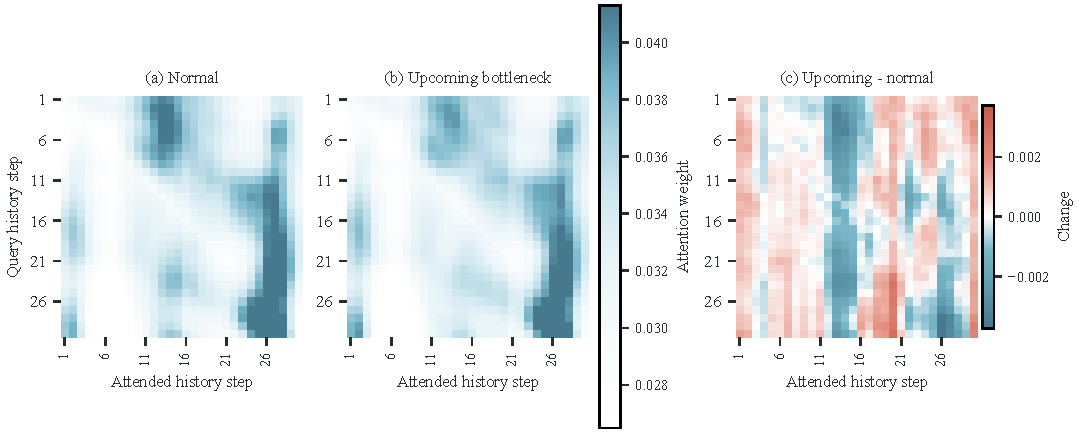
\includegraphics[width=0.98\textwidth]{figures/attention_heatmaps/fig04_temporal_attention_states.pdf}
\caption{Temporal attention over 30 history windows: (a)~normal; (b)~upcoming; (c)~upcoming-minus-normal.}
\label{fig:attn-temporal}
\end{figure*}
\begin{figure*}[t]
\centering
\includegraphics[width=0.92\textwidth]{figures/attention_heatmaps/fig05_layerwise_upcoming_attention_selected.pdf}
\caption{Geographic (upper) and semantic (lower) attention in selected encoder layers 1, 4, and 5.}
\label{fig:attn-layers}
\end{figure*}
\begin{figure*}[t]
\centering
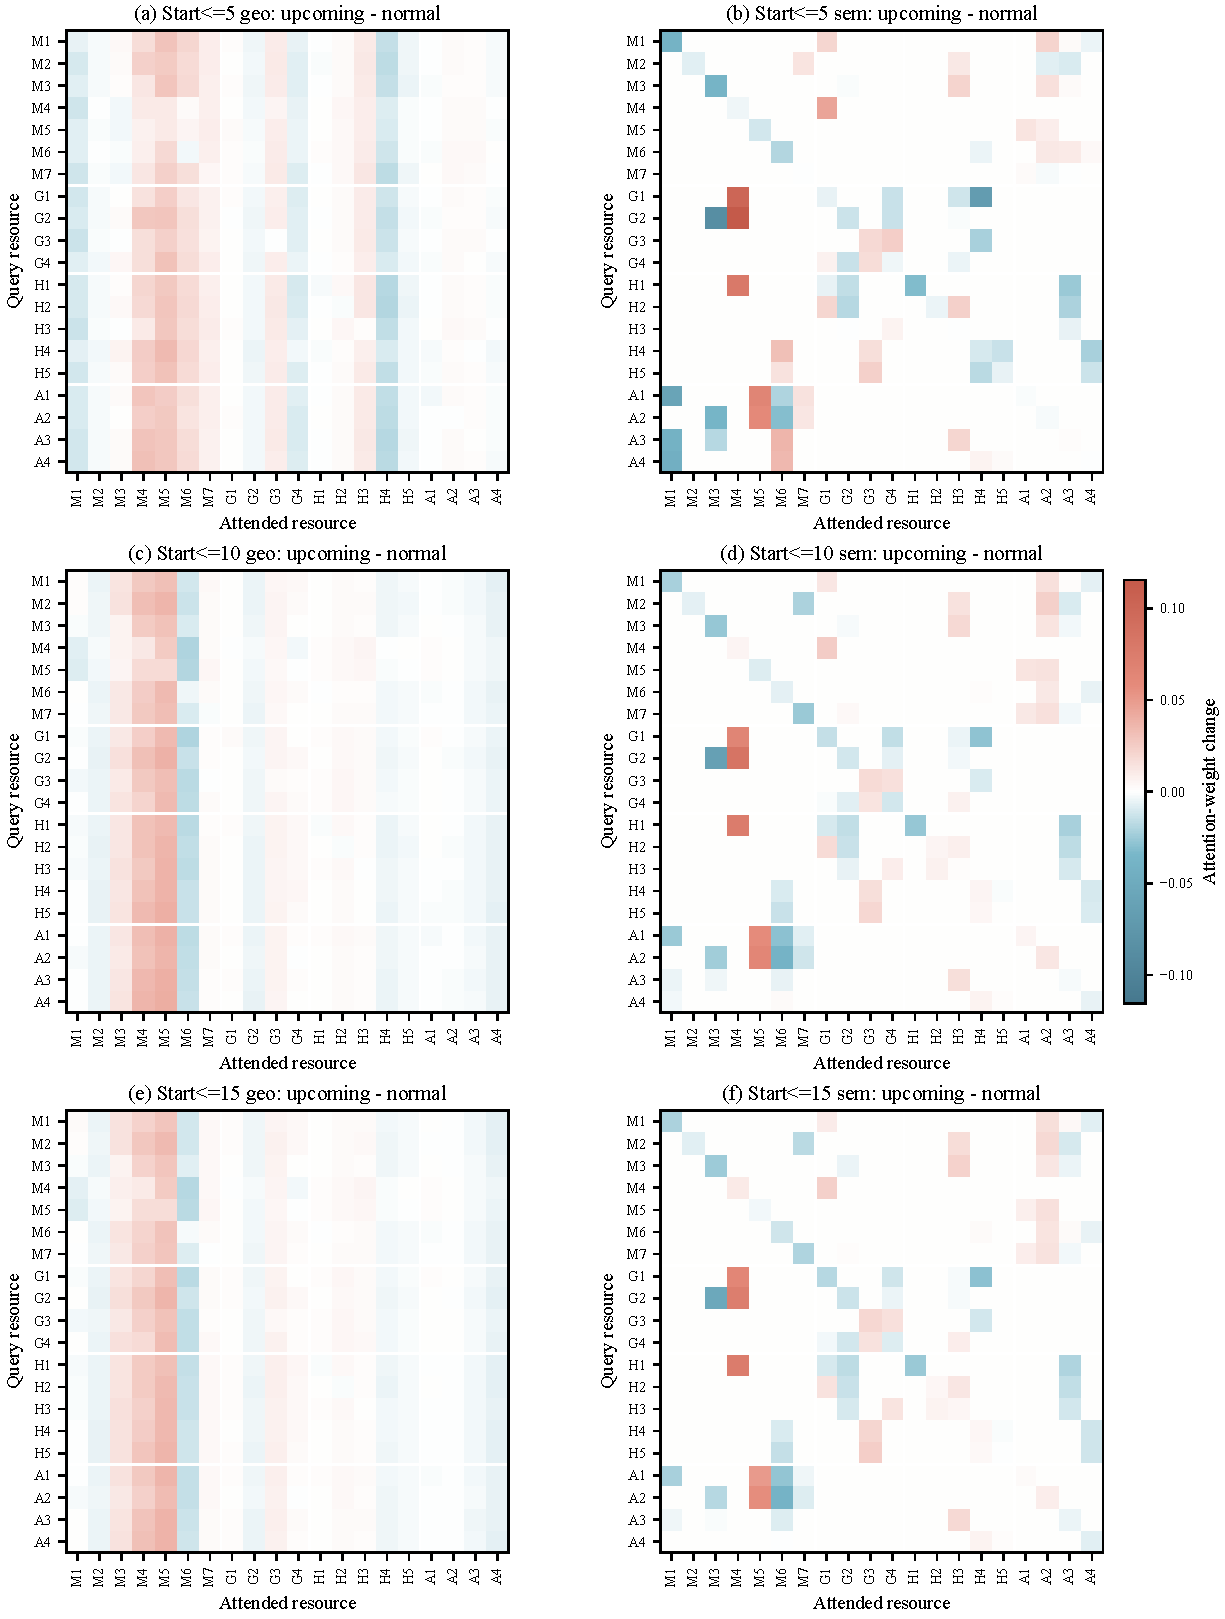
\includegraphics[width=0.98\textwidth]{figures/attention_heatmaps/fig07_horizon_attention_change.pdf}
\caption{Upcoming-minus-normal attention change across Start caps 5/10/15 (upper: geographic; lower: semantic).}
\label{fig:attn-horizons}
\end{figure*}


\subsubsection{Decoder and training components}\label{sec:decoder-training}

The decoder and training comparisons examine two requirements of advance warning: distinguishing new events from continuing events and maintaining sensitivity to distant onsets. NoSplit replaces the continuation and onset heads with one shared head, while NoFarBoost removes far-onset weighting and the associated enhanced false-alarm penalty. Both arms retain the common initialization, 50-epoch curriculum, and validation-controlled checkpoint and threshold-selection rule. Table~\ref{tab:decoder-ablation} reports the resulting operating points.

\begin{table*}[t]
\centering
\caption{Ablation of the split event heads and the far-onset enhancement. Distance-specific $R_{\mathrm{up,rep}}$ additionally requires the three-window onset tolerance. Thr is the validation-selected report threshold.}
\label{tab:decoder-ablation}
\scriptsize
\setlength{\tabcolsep}{3.5pt}
\renewcommand{\arraystretch}{1.08}
\begin{tabular*}{\FullWidth}{@{\extracolsep{\fill}}llrrrrrr@{}}
\toprule
Arm & Start cap & Thr & F1-score & Upcoming R & $R_{\mathrm{up,rep}}^{>10}$ & Ongoing R & Dur.\ MAE \\
\midrule
Full & $\leq5$ & 94.0\% & 80.4\% & 54.2\% & --- & \textbf{93.7\%} & 4.17 \\
NoFarBoost & & 90.0\% & \textbf{81.9\%} & \textbf{54.5\%} & --- & 92.3\% & \textbf{4.03} \\
NoSplit & & 94.0\% & 72.7\% & 19.0\% & --- & 93.5\% & 5.56 \\
\midrule
Full & $\leq10$ & 94.0\% & \textbf{77.8\%} & 53.5\% & --- & 93.9\% & \textbf{4.38} \\
NoFarBoost & & 88.0\% & 75.2\% & \textbf{56.0\%} & --- & 92.3\% & 4.66 \\
NoSplit & & 94.0\% & 58.0\% & 24.7\% & --- & \textbf{94.7\%} & 6.63 \\
\midrule
Full & $\leq15$ & 94.0\% & \textbf{76.8\%} & \textbf{53.7\%} & \textbf{43.3\%} & 93.0\% & \textbf{4.43} \\
NoFarBoost & & 94.0\% & 74.1\% & 48.9\% & 24.0\% & 92.5\% & 4.87 \\
NoSplit & & 94.0\% & 58.6\% & 35.3\% & 12.5\% & \textbf{95.1\%} & 6.36 \\
\bottomrule
\end{tabular*}
\end{table*}

Separating onset and continuation decisions gives PHGST-PD Upcoming recall of $0.542/0.535/0.537$, compared with $0.190/0.247/0.353$ for the shared head; NoSplit's Ongoing recall remains $0.935$--$0.951$. The contrast localizes the value of separate decisions to emerging events. Far-onset enhancement concentrates its benefit at the 10- and 15-min caps, where PHGST-PD records F1-score $0.778/0.768$ and union duration MAE $4.38/4.43$~min, compared with $0.752/0.741$ and $4.66/4.87$~min for NoFarBoost. Strict report recall for events beyond 10~min rises from $0.240$ to $0.433$. At the 5-min cap, NoFarBoost records F1-score $0.819$ and union MAE $4.03$~min, at threshold $0.90$ versus $0.94$ for PHGST-PD. This range-dependent pattern motivates the enhancement for longer warning distances. On the key-device trace (Figure~\ref{fig:key-device-struct-graph}), PHGST-PD reaches 15--17~min during the displayed 20-min reference plateau and follows its decay; the structural variants peak at 12--14.5~min and show post-event spikes.

Head-specific stage-2 fine-tuning reduces overall order remaining-time MAE by $1.32/1.94/0.81$~min at Start$\leq5/10/15$, respectively (Figure~\ref{fig:remain-finetune}). The phase-resolved comparison shows that the reduction is concentrated in early production, where MAE falls by $2.70/3.49/1.64$~min, and remains positive in the middle phase. Late-production MAE changes by only $+0.09/-0.13/+0.01$~min, indicating that the aggregate gain comes primarily from the more difficult early and middle windows rather than a uniform shift across the order trajectory. The event and cause heads remain frozen during this fine-tuning stage.

\begin{figure*}[t]
\centering
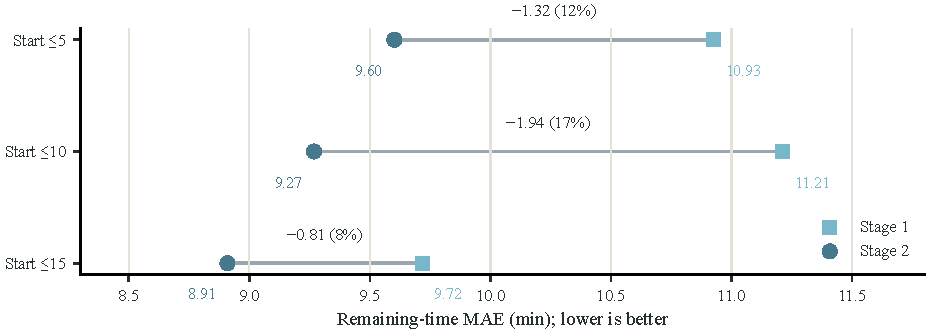
\includegraphics[width=0.90\textwidth]{figures/fig_remain_dumbbell.pdf}
\caption{Effect of remaining-time fine-tuning across early, middle, and late production phases (blue: MAE decrease; coral: increase).}
\label{fig:remain-finetune}
\end{figure*}
\begin{figure*}[t]
\centering
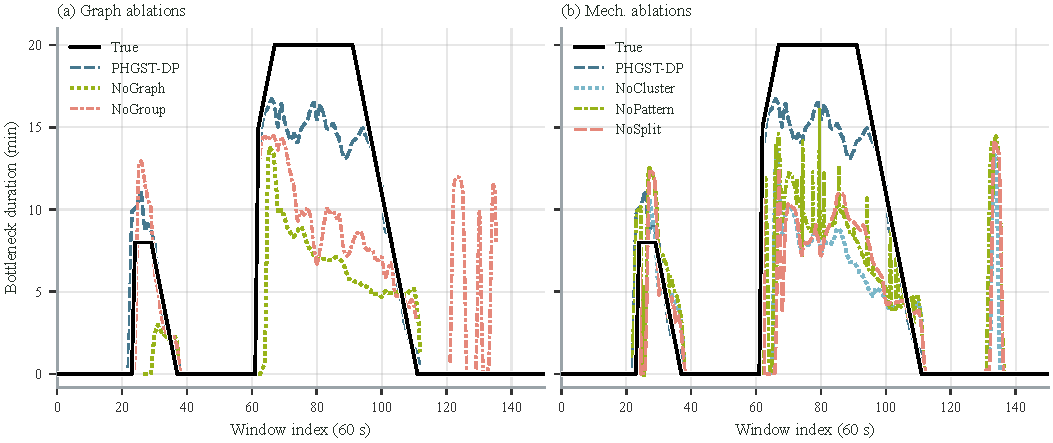
\includegraphics[width=0.96\textwidth]{figures/key_device_struct_pair.pdf}
\caption{Key-device ablation traces (Start$\leq5$): (a)~graph arms; (b)~process-rule/context, the propagation-delay-aware module, and decoder arms.}
\label{fig:key-device-struct-graph}
\end{figure*}

\paragraph*{Supplementary development diagnostics.}
One non-test diagnostic is retained for transparency. Appendix~\ref{app:checkpoint-validation} records validation event metrics at the selected checkpoints (Table~\ref{tab:checkpoint-validation-event}). These values document model selection and are not used as held-out evidence of PHGST-PD superiority.

\subsection{Case study and process traceability}

The case study shows how an event report follows bottleneck onset, persistence, and recovery on a production resource. The selected roller-bed CNC pipe-intersection cutting workstation (\texttt{num02}) contributes 301 event-positive window--resource pairs in the test set. Device and episode selection follows a fixed rule: among devices with at least the median event count, select the device with the most events in one episode (ties resolved by PHGST-PD one-step F1), then select its episode with the most and longest bottleneck segments. The resulting episode, \texttt{n10\_human1.0\_\_episode\_03}, contains an approximately 8-min bottleneck and a 49-min bottleneck. The prediction horizon remains 30~min. For visualization, the true-duration reference in the key-device plots is truncated at 20~min to emphasize onset and recovery; the omitted 20--30~min range does not change the experimental prediction horizon. PHGST-PD detects both intervals and tracks their recovery (Figure~\ref{fig:key-device-baselines}). The short event is reported about 1~min in advance with a 10--11~min duration estimate; the long event's onset is aligned, and its declining duration is followed. During the displayed reference plateau, predicted duration is 13--17~min, and state mismatches occur at onset and recovery boundaries (1--2 windows each). The trace illustrates how the report combines event notification with a continuously updated duration estimate.

\begin{figure*}[t]
\centering
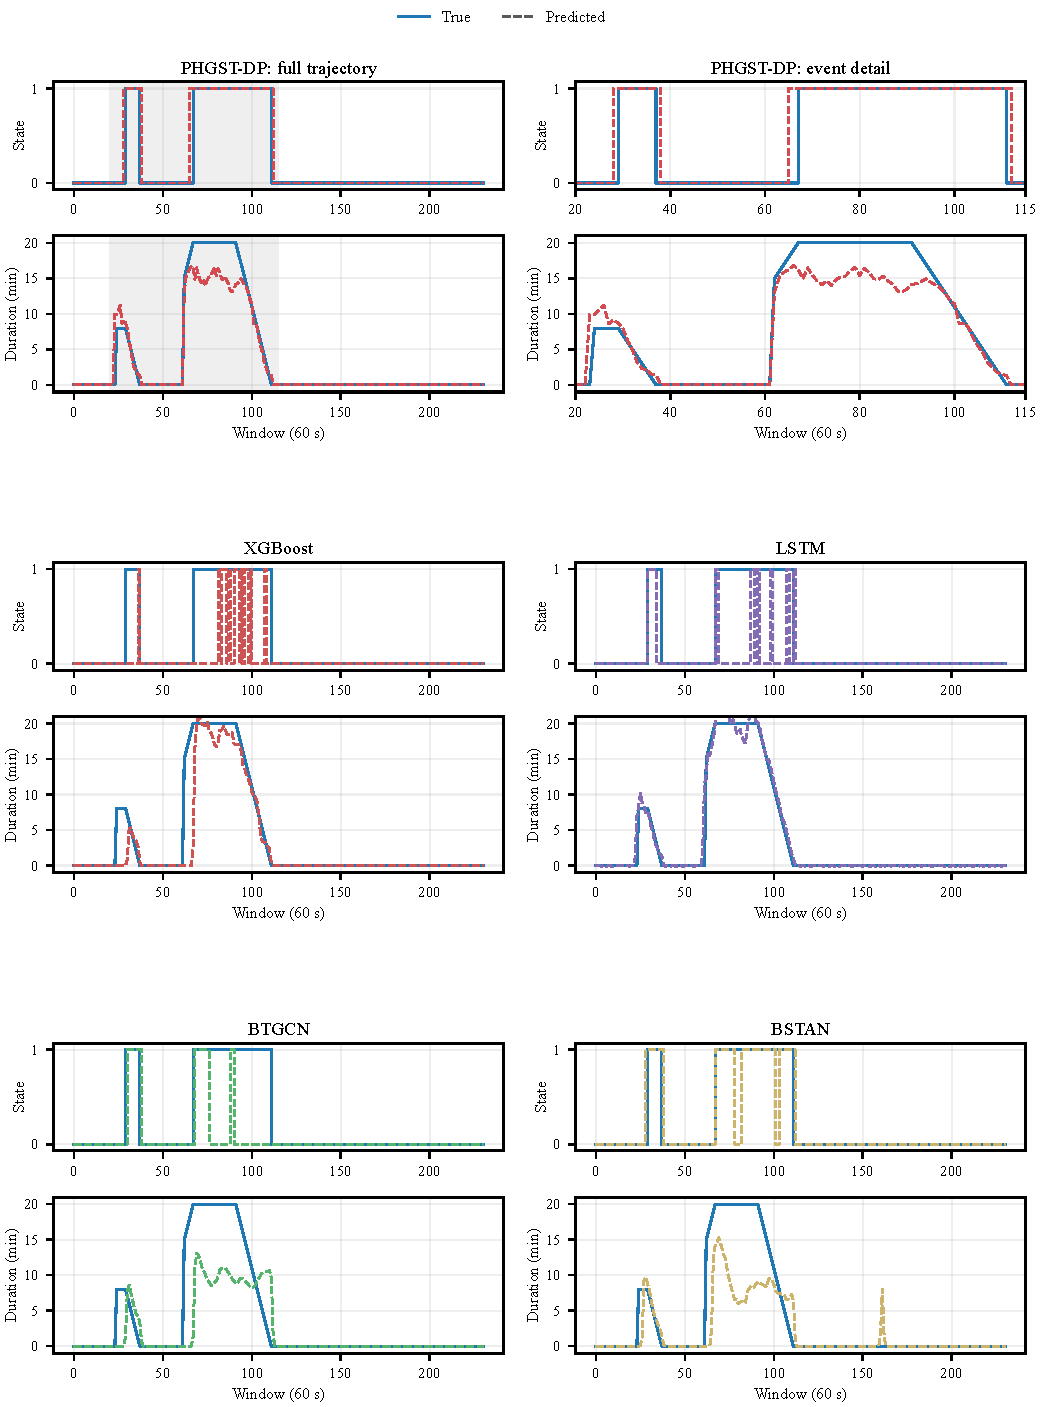
\includegraphics[width=0.96\textwidth]{figures/key_device_models_aligned.pdf}
\caption{Key-device comparison of PHGST-PD and baselines at Start$\leq5$: (a)~next-window state; (b)~duration with the true reference truncated at 20~min for visualization (black: true; dashed: predictions).}
\label{fig:key-device-baselines}
\end{figure*}

Figure~\ref{fig:key-device-baselines} overlays PHGST-PD with XGBoost, LSTM, BTGCN, and BSTAN on the same device and episode: next-window state on the left and duration on the right. Black solid lines show the targets; dashed predictions use one colour per method. Window indices start after the 30-window history. PHGST-PD maintains continuous state coverage over both bottleneck intervals and follows the duration decline towards recovery, while the baselines show gaps or weaker duration tracking on the same trajectory. The aggregate event and temporal results are reported in Table~\ref{tab:comparison-main}.

The all-resource view connects these local traces to coordinated production-state prediction. Figure~\ref{fig:all-devices-main} shows the seven workstation targets in the same episode. That episode contains 64 positive bottleneck cells, the highest count among test episodes, and all of them fall on these workstations. PHGST-PD recovers every positive cell of the cutting workstation and second welding station (\texttt{num00\_weld\_ws1}), with episode-level State F1 $0.941$. Light-blue cells denote true positives; red cells denote false positives and false negatives. The corresponding F1 values are $0.855$ for NoInfo, $0.832$ for NoCluster, and $0.901$ for NoGraph. NoInfo and NoCluster omit the welding-station interval, while NoGraph fragments it. In this episode, the full model maintains coverage across both resources, while the ablated variants miss or fragment the welding-station interval.

\begin{figure}[pos=htbp]
\centering
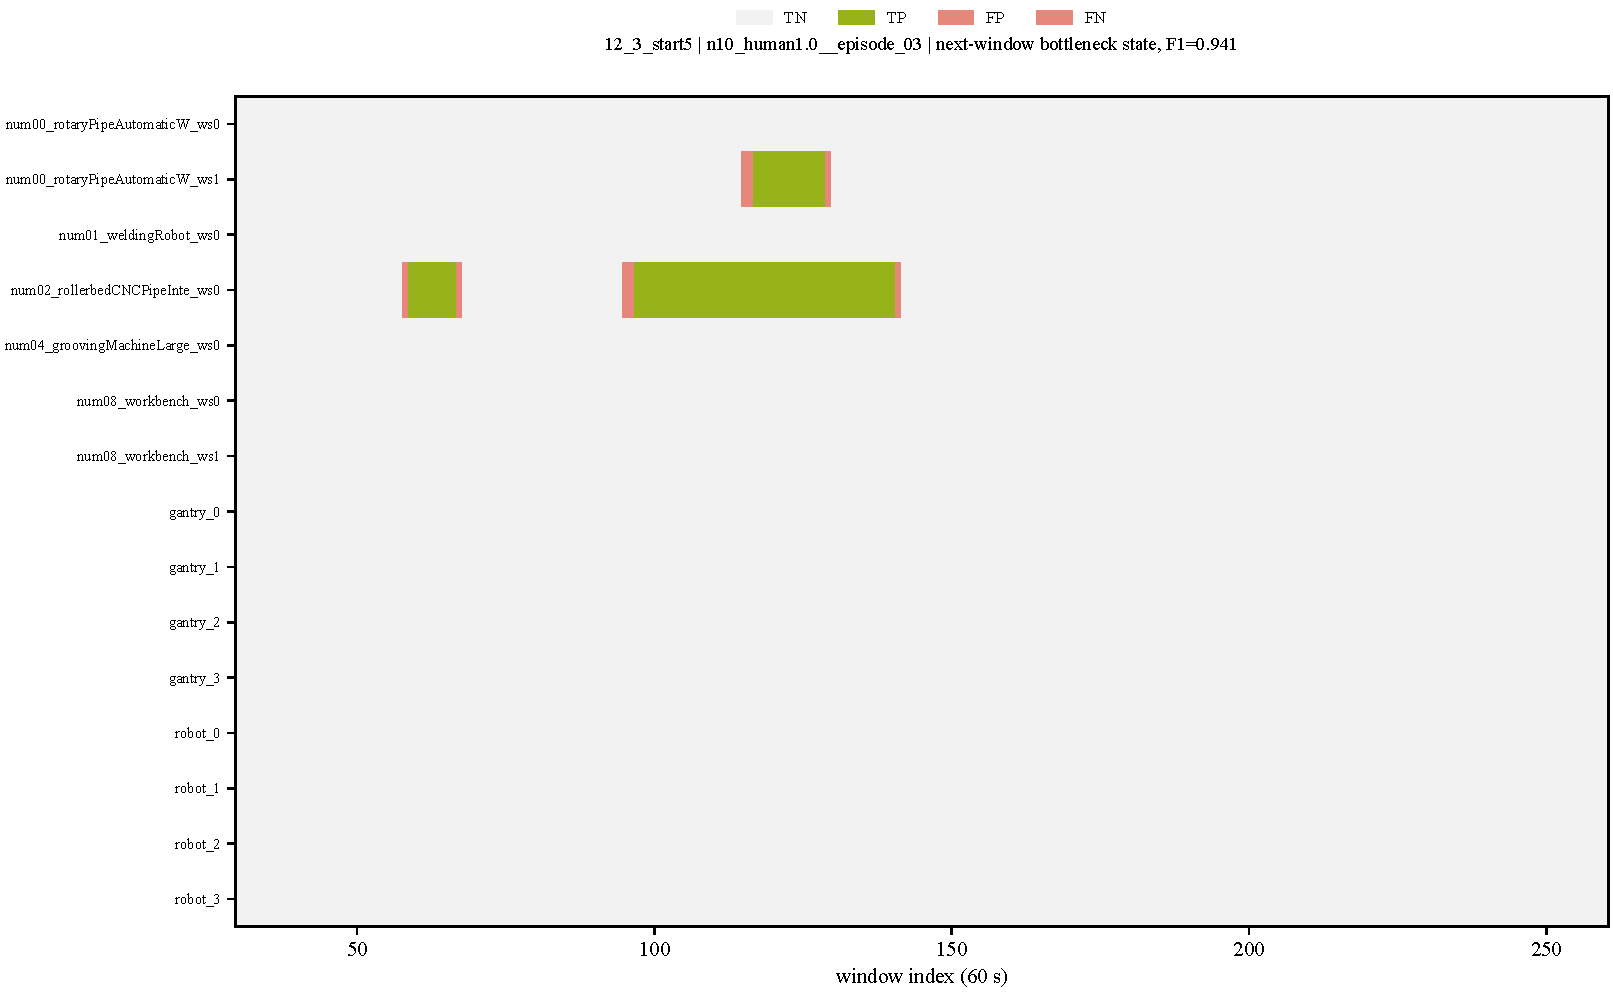
\includegraphics[width=\columnwidth]{figures/all_devices_state_main.pdf}
\caption{Next-window state map for seven workstation targets (gray TN; light blue TP; coral FP/FN).}
\label{fig:all-devices-main}
\end{figure}

On the full Start$\leq5$ test split, support is uneven across the 15 targets (Figure~\ref{fig:per-device}). The cutting workstation contributes 301 true events, while AGV~2 and AGV~3 contribute none and are excluded from the box statistics. F1 on the supported devices ranges from $0.535$ on the welding robot to $0.964$ on bench~ws1. This split is a coverage check for one checkpoint, not a claim that every resource family is equally predictable.

\begin{figure*}[t]
\centering
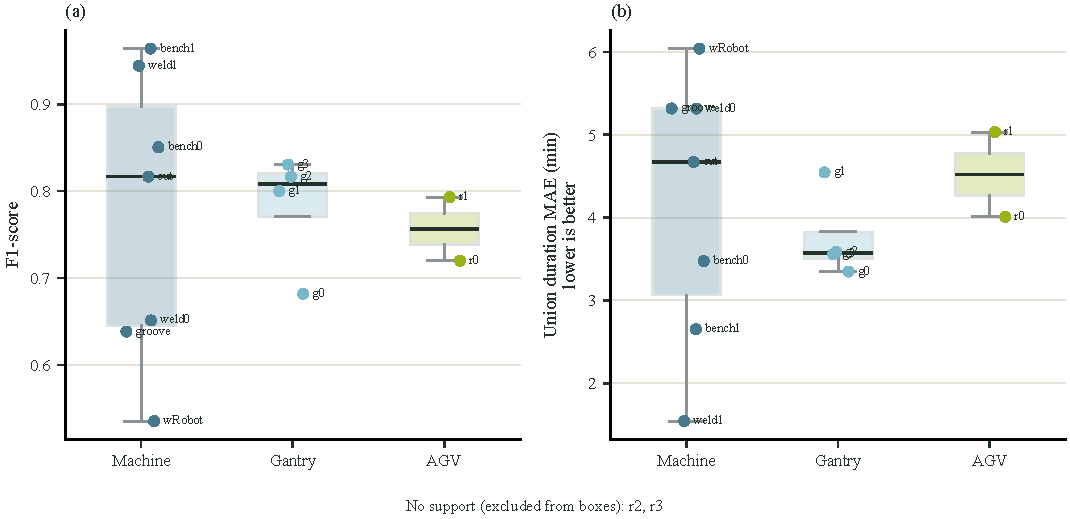
\includegraphics[width=0.96\textwidth]{figures/fig_per_device_box.pdf}
\caption{Per-device F1-score and union duration MAE for PHGST-PD at Start$\leq5$, by workstation, gantry, and AGV.}
\label{fig:per-device}
\end{figure*}

Process-cause outputs link a predicted event to interpretable production symptoms: material shortage, transport delay, queue buildup, and downstream blockage. The labels encode process-rule evidence, so the explanation is an association with observed operating conditions. Together with the event and state traces, these outputs provide a resource, a time interval, and a process context for reviewing a predicted constraint.

\paragraph*{Mixed-condition probability map.}
Figure~\ref{fig:attn-prediction} extends the single-resource trajectory to a supplementary mixed-condition episode, \texttt{n10\_mix\_all1.0\_\_episode\_03}. It is selected automatically for high bottleneck activity and displays relative test-window indices $0$--$200$ from the Start$\leq5$ mixed-condition checkpoint. The three aligned panels retain the future-event labels, model probabilities and absolute probability errors. Visible mismatches include probabilities on resources without a corresponding positive label as well as incomplete coverage of labelled intervals. The probability map is distinct from a thresholded operational report. Its 20 displayed rows contain the 15 evaluation targets and five worker context nodes; the 18 buffer rows are omitted for readability. It therefore illustrates where this supplementary model agrees or disagrees with labels; it is not an aggregate performance result for the retained \texttt{dense\_i1} model.

\begin{figure}[pos=htbp]
\centering
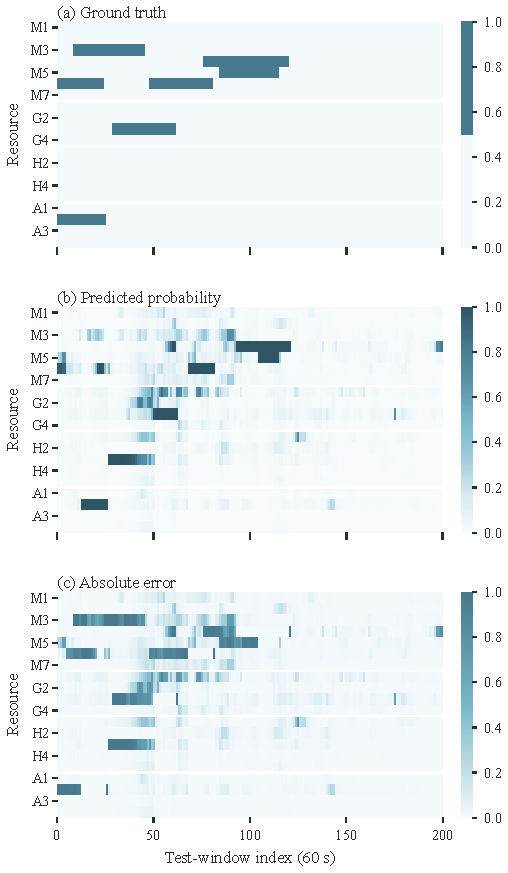
\includegraphics[width=\columnwidth]{figures/attention_heatmaps/fig08_prediction_heatmaps.pdf}
\caption{Future-event labels, predicted probabilities, and absolute errors for a mixed-condition episode (Start$\leq5$).}
\label{fig:attn-prediction}
\end{figure}

\paragraph*{Resource-level coverage.}
The overall Start$\leq5$ event F1-score is $80.4\%$, using the same onset-qualified matching criterion as Table~\ref{tab:comparison-main}. Table~\ref{tab:complete-6-1} retains the individual resource counts, F1-score, and duration errors behind the case analysis. It shows which workstations and handling resources contribute to the aggregate result; \texttt{robot\_2} and \texttt{robot\_3} have zero true events and are omitted.

% Author confirms overall F1 = 80.4 percent and the same matching criterion as the main table.
% Per-device server exports are pending synchronization; do not infer replacement device counts from the aggregate score.
\begin{table*}[pos=!tbp]
\centering
\scriptsize
\setlength{\tabcolsep}{3pt}
\renewcommand{\arraystretch}{1.12}
\caption{Per-device event and duration performance at Start$\leq5$. Durations are in minutes. Zero-support resources (\texttt{robot\_2}, \texttt{robot\_3}) are omitted.}
\label{tab:complete-6-1}
\begin{tabularx}{\textwidth}{@{}lXXXXXXX@{}}
\toprule
Device & $n_{\mathrm{true}}$ & $n_{\mathrm{pred}}$ & $P$ & $R$ & F1-score & Dur MAE & Dur RMSE \\
\midrule
num00\_weld\_ws0 & 115 & 100 & 70.0\% & 60.9\% & 65.1\% & 5.31 & 7.11 \\
num00\_weld\_ws1 & 17 & 19 & 89.5\% & 100.0\% & 94.4\% & 1.54 & 2.76 \\
num01\_robotweld\_ws0 & 46 & 25 & 76.0\% & 41.3\% & 53.5\% & 6.04 & 7.56 \\
num02\_CNC$^\ast$\_ws0 & 301 & 343 & 76.7\% & 87.4\% & 81.7\% & 4.67 & 6.45 \\
num04\_groove\_ws0 & 20 & 27 & 55.6\% & 75.0\% & 63.8\% & 5.32 & 6.87 \\
num08\_bench\_ws0 & 186 & 162 & 91.4\% & 79.6\% & 85.1\% & 3.47 & 5.02 \\
num08\_bench\_ws1 & 94 & 101 & 93.1\% & 100.0\% & 96.4\% & 2.65 & 3.65 \\
gantry\_0 & 18 & 26 & 57.7\% & 83.3\% & 68.2\% & 3.35 & 4.85 \\
gantry\_1 & 31 & 34 & 76.5\% & 83.9\% & 80.0\% & 4.55 & 6.45 \\
gantry\_2 & 108 & 132 & 74.2\% & 90.7\% & 81.7\% & 3.59 & 5.56 \\
gantry\_3 & 121 & 127 & 81.1\% & 85.1\% & 83.1\% & 3.56 & 5.04 \\
robot\_0 & 15 & 10 & 90.0\% & 60.0\% & 72.0\% & 4.01 & 6.14 \\
robot\_1 & 30 & 28 & 82.1\% & 76.7\% & 79.3\% & 5.03 & 6.80 \\
\bottomrule
\end{tabularx}
\end{table*}


\subsection{Prediction quality and computational cost}\label{sec:efficiency}

This experiment evaluates the computation required to deliver the predictive quality reported in Section~\ref{sec:comparison-event}. All five models perform inference on an NVIDIA GeForce RTX~5090. The environment uses Python~3.11.15 and CUDA~12.8, with PyTorch~2.11.0 for the neural models and XGBoost~3.2.0 with CuPy~14.2.0 for the seven tree-based prediction heads. Throughput is measured over five complete test passes at batch size 16 after 50 warm-up batches. Forward and report latency use batch size 1 and 5,000 timed calls, with CUDA synchronization before and after each measurement. The timing boundary covers model-side reporting. Forward timing covers prediction with inputs or prepared features resident on the GPU. Report timing includes input transfer, model-specific feature processing, prediction, and event-report generation; for XGBoost, this includes CPU history-feature construction, host-to-device transfer, seven CUDA prediction heads, and device-to-host output transfer. Batched test passes also include data loading. Table~\ref{tab:efficiency} summarizes the three onset caps, and Figure~\ref{fig:quality-cost} relates report latency to the F1-score values in Table~\ref{tab:comparison-main}.

% All 15 GPU timing rows are verified against isaac_factory@a5b6c92,
% including the original PHGST-PD report snapshots. B2 uses the 2026-10-24 CUDA run.
% See experiments/efficiency_comparison_2026-10-24.md for provenance and checks.
\begin{table*}[t]
\centering
\caption{Inference cost on the RTX~5090. Ranges give the minimum and maximum across Start $\leq5$, $\leq10$, and $\leq15$ min. Throughput uses batch size 16 and report latency uses batch size 1. GPU allocation is the PyTorch allocator peak.}
\label{tab:efficiency}
\footnotesize
\setlength{\tabcolsep}{3.3pt}
\renewcommand{\arraystretch}{1.15}
\begin{tabular*}{\FullWidth}{@{\extracolsep{\fill}}lrrrrrr@{}}
\toprule
Model & Parameters & \makecell{GPU allocation\\(MiB)} & \makecell{Throughput $\uparrow$\\(samples/s)} & \makecell{Report p50 $\downarrow$\\(ms)} & \makecell{Report p95 $\downarrow$\\(ms)} & \makecell{Report p99 $\downarrow$\\(ms)} \\
\midrule
\textbf{PHGST-PD} & 713,984 & 175.8 & 1,946\textendash{}1,987 & 4.72\textendash{}4.77 & 5.32\textendash{}5.41 & 5.51\textendash{}5.60 \\
XGBoost & \na & \na & 236\textendash{}323 & 39.29\textendash{}58.55 & 41.73\textendash{}60.86 & 52.81\textendash{}72.66 \\
LSTM & 752,867 & 83.8 & 8,547\textendash{}8,740 & 0.64\textendash{}0.65 & 1.14\textendash{}1.15 & 1.33\textendash{}1.35 \\
BTGCN & 274,339 & 240.3 & 6,881\textendash{}7,274 & 0.92\textendash{}0.95 & 1.48\textendash{}1.51 & 1.62\textendash{}1.66 \\
BSTAN & 287,267 & 239.7 & 6,584\textendash{}6,667 & 1.00\textendash{}1.03 & 1.54\textendash{}1.58 & 1.64\textendash{}1.68 \\
\bottomrule
\end{tabular*}
\par\vspace{3pt}
\begin{minipage}{\FullWidth}
\scriptsize
Timing runs use the source-recorded workloads on a shared server under the same unified 5,354-window re-evaluation as Section~\ref{sec:comparison-overview}. GPU allocation includes resident inference inputs. XGBoost uses its native CUDA allocator, so its PyTorch allocation is unavailable; its separately sampled NVML process peak is 662--670~MiB, including the CUDA context, libraries, and caches.
\end{minipage}
\end{table*}

\begin{figure*}[t]
\centering
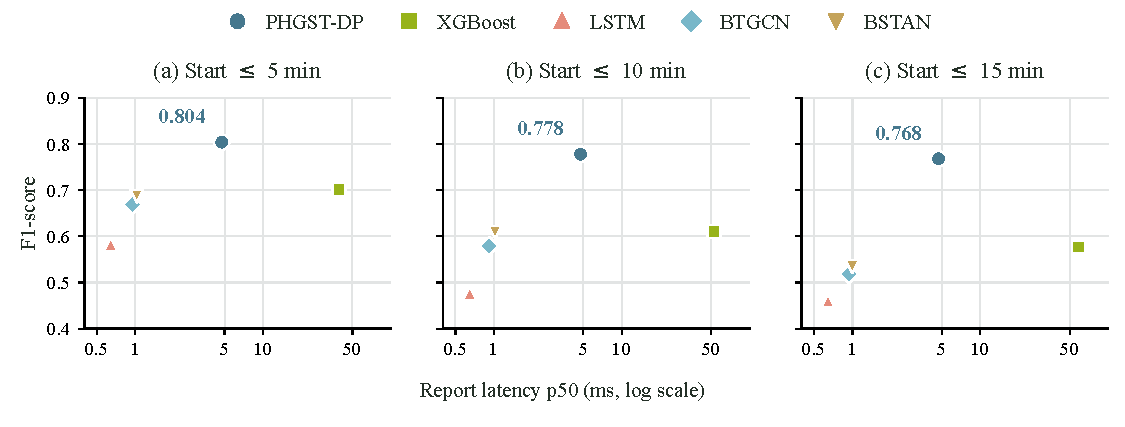
\includegraphics[width=0.96\textwidth]{figures/fig_quality_cost.pdf}
\caption{Event-identification quality versus median report latency for each onset cap.}
\label{fig:quality-cost}
\end{figure*}

PHGST-PD combines F1-score of $0.804/0.778/0.768$ with median report latency of 4.72--4.77~ms and p99 latency of 5.51--5.60~ms. Figure~\ref{fig:quality-cost} places it at the highest F1-score for each onset cap with millisecond-scale reporting. XGBoost's measured CUDA implementation has report p50 of 39.29--58.55~ms and p99 of 52.81--72.66~ms; LSTM, BTGCN, and BSTAN have median report latency below 1.1~ms. These measurements show the trade-off between predictive quality and report latency across the evaluated implementations. PHGST-PD's heterogeneous resource interactions and propagation-delay-aware module fit within a model-side reporting budget far shorter than the 60-s observation interval, making its event coverage and advance warning usable within the studied update cycle.

The resource requirements remain stable across onset caps. PHGST-PD processes 1,946--1,987 samples/s, with a 0.05-ms spread in median report latency. Its 713,984 parameters occupy a 2.91-MiB checkpoint, and peak GPU allocation is approximately 175.8~MiB, about 27\% below BTGCN and BSTAN under the measured configurations; LSTM uses 83.8~MiB. The three checkpoints share the same architecture and input shape. This combination of a compact parameter set, stable inference cost, and detailed event predictions supports frequent report updates on the tested platform.

\section{Discussion}\label{sec:discussion}

The experiments show that PHGST-PD can combine advance warning with a detailed description of emerging bottlenecks in the evaluated multi-entity production environment. The baseline comparisons support improved event identification together with onset, duration, and production-state forecasting (Table~\ref{tab:comparison-main}), while the resource-level cases show how these outputs follow bottleneck onset, persistence, and recovery. Jointly reporting the affected resource, event interval, observable process cause, and remaining order time gives the forecast a production meaning beyond an isolated bottleneck score. The resulting contribution is an integrated description of where and when a constraint is expected, how long it may persist, and what operational context accompanies it.

The component studies assess how the three methodological contributions affect predictive performance. First, the heterogeneous process--logistics graph allows the predictor to use workstation, worker, buffer, and transport information jointly. The graph and cross-resource ablations particularly affect upcoming-event recall, supporting the use of related-resource observations before a target becomes constrained (Table~\ref{tab:entity-ablation-new}). Second, process-informed supervision connects event and cause targets to observable production evidence, while temporal pattern clustering summarizes recurrent operating histories. The matched-budget cause study shows that the clearest benefit of cause supervision is improved process interpretation, with little change in station identification (Table~\ref{tab:matched-cause}). Third, the propagation-delay-aware module uses the temporal-pattern context in cross-resource attention. Removing pattern matching reduces warning coverage for more distant onsets (Table~\ref{tab:delay-ablation-new}), supporting its predictive role in using lagged information. This evidence concerns forecast behaviour; it does not establish that attention recovers physical propagation paths or estimates actual propagation times.

The report outputs can inform complementary production decisions. Resource and onset forecasts help determine where and when to direct attention; duration estimates help assess the available intervention window; process-cause outputs suggest conditions to inspect; and remaining-time estimates provide context for order-progress assessment. The model-side latency results support updating these reports within the studied one-minute observation cycle (Section~\ref{sec:efficiency}). A deployment interface could map observations from manufacturing execution systems (MES), warehouse management systems (WMS), and transport-dispatch systems to the resource graph, consistent with integrated monitoring and simulation platforms for reconfigurable manufacturing systems~\cite{leng2023monitoring}. Whether such information improves scheduling or throughput depends on the intervention policy and available resources and requires separate closed-loop evaluation.

The current evaluation uses an open-workspace factory environment developed for NVIDIA Isaac Sim. Transfer across layouts, products, and physical factories remains to be evaluated. Future work will extend validation to physical production systems and closed-loop resource interventions, examining how the forecasts support production decisions and measurable performance improvements.

\section{Conclusion}\label{sec:conclusion}

This study presents PHGST-PD for dynamic bottleneck prediction in multi-entity production systems. A heterogeneous process--logistics graph broadens the observed resource interactions, process-informed supervision and temporal pattern clustering organize event targets and recurrent operating context, and a propagation-delay-aware module uses historical cross-resource information for prediction. Experiments in the evaluated factory environment show improved event-prediction accuracy relative to the compared baselines, while ablations and production traces support the roles of these components in advance warning and temporal tracking. By jointly reporting bottleneck station, onset, duration, observable process cause, and remaining order time, PHGST-PD provides detailed forecasts that can inform timely resource interventions. Further validation in physical production systems is needed to determine whether these forecasts improve intervention decisions and production outcomes.

\printcredits

\section*{Declaration of Competing Interest}
The authors declare that they have no known competing financial interests or personal relationships that could have appeared to influence the work reported in this paper.

\section*{Data availability}
Data will be made available on request.

\section*{Acknowledgments}
The work described in this paper is supported by grants from RGC General Research Fund (17206126), Technology Cooperation Funding Scheme (TCFS) (Ref No.\ GHP/321/22SZ), The University of Hong Kong (Ref No.\ 2407102267, 2503252159), and Innovation and Technology Fund (ITF) (Ref No.\ TP/041/24LP).

%% Bibliography precedes the appendix, following common Elsevier layout.
\bibliographystyle{unsrtnat}
\bibliography{../cas-refs}

\clearpage
\appendix
\onecolumn
\section{Implementation details and additional results}\label{app:additional}

This appendix collects complementary numerical tables and the complete attention visualizations that underlie the main-text figures. The materials are intended for cross-checking rather than as a substitute for the primary comparisons in Section~\ref{sec:exp}.

\paragraph{Shared training and evaluation protocol.}
\label{app:shared-protocol}
Table~\ref{tab:shared-training-protocol} records the controls held fixed across the reported Full model and ablation arms. Architectural switches listed in Table~\ref{tab:ablation-arms} are the intended differences between arms; initialization, optimization budget, curriculum, validation-based model selection, and held-out evaluation otherwise follow the common protocol below.

\begin{table}[pos=htbp]
\centering
\caption{Shared training and evaluation protocol for the Full model and all ablation arms.}
\label{tab:shared-training-protocol}
\small
\setlength{\tabcolsep}{6pt}
\renewcommand{\arraystretch}{1.10}
\begin{tabularx}{\textwidth}{@{}lX@{}}
\toprule
Item & Shared setting \\
\midrule
Initialization & Identical initial parameter values for the Full model and every ablation arm \\
Random seed & 42 \\
Optimizer & AdamW \\
Batch size & 16 \\
Learning rate & $5\times10^{-5}$ initially; cosine decay to $10^{-6}$ \\
Weight decay & 0.05 \\
Positive-window sampling & Fourfold oversampling \\
Maximum training budget & 50 epochs for each Start-cap run \\
Early stopping & Patience of 40 epochs \\
Curriculum & Start$\leq5\rightarrow$Start$\leq10\rightarrow$Start$\leq15$ \\
Checkpoint criterion & Validation station-identification F1 among candidates satisfying report precision $\geq0.80$ and recall $\geq0.70$ \\
Threshold candidates & $\{0.45,0.50,0.55,0.60,0.65,0.70,0.75,0.80,0.85,0.88,0.90,0.94\}$ \\
Held-out evaluation & The selected checkpoint and threshold are frozen before the shared test episodes are evaluated \\
\bottomrule
\end{tabularx}
\end{table}

\begin{table}[pos=htbp]
\centering
\caption{Shared model, windowing, event, and decoding parameters.}
\label{tab:model-task-parameters}
\small
\setlength{\tabcolsep}{6pt}
\renewcommand{\arraystretch}{1.10}
\begin{tabularx}{\textwidth}{@{}lX@{}}
\toprule
Item & Setting \\
\midrule
Temporal resolution & 60~s per window \\
Input and prediction ranges & 30 historical windows and a 30-window future grid \\
Prediction targets & 15 resources: seven workstations, four gantries, and four transport robots \\
Event construction & Minimum eight-window persistence; one-window internal gap filling \\
Onset caps and matching tolerance & Start$\leq5/10/15$ windows; three-window onset tolerance \\
Encoder & Five blocks; 80-dimensional hidden representation \\
Attention heads & Temporal/geographic/semantic: $4/2/2$ \\
Graph and semantic context & Geographic hop-distance cutoff of 4; five semantic neighbours \\
Positional encoding & Eight-dimensional Laplacian encoding \\
Temporal-pattern prototype bank & 16 prototypes; length-three temporal patches \\
Far-onset enhancement & Onset-loss multiplier 2; positive weights $9/10/11$ for Start$\leq5/10/15$ \\
False-alarm weighting & 2.5 for ordinary false positives; additional hard-false-positive multiplier 2.2 \\
\bottomrule
\end{tabularx}
\end{table}


\paragraph{Additional implementation parameters.}
\label{app:implementation-parameters}
The configuration expands the objective in Section~\ref{sec:method} as follows. Event occurrence, start, duration, and prefix losses have weights $2.4$, $2.0$, $2.0$, and $2.5$, respectively. The cold-history onset term has weight $2.2$ within the event-occurrence objective; focal modulation uses exponent $1.5$, and the internal differentiable F1 term has weight $0.8$. Future occupancy uses separate binary-cross-entropy, Dice, and IoU weights of $0.7$, $0.5$, and $0.35$. The reconstruction, supervised contrastive, cause, and turning-point/momentary losses have weights $0.2$, $0.05$, $0.1$, and $0.25$. Remaining-time regression has weight $0.5$ in stage~1 and $4.0$ during head-only stage~2. The legacy score, will, mark, time-to-start, STGNPP, and offline cluster objectives have zero weight. These coefficients distinguish the active event-occurrence loss from the disabled legacy will objective.

\paragraph{Numerical operational-state thresholds.}
All state rules act on the original physical feature scale before input standardization. Let $q$, $B$, $S$, $U$, $I$, $R$, and $Z$ denote queue length, blocked seconds, starved seconds, unavailable fraction, inbound-wait seconds, route-delay seconds, and shortage propagation, respectively. At the 60-s resolution, a workstation has raw hot evidence if any of the following holds: (i) $q\geq2$ and $B+S>0$; (ii) $B\geq24$ and $q\geq1$; (iii) $B+S\geq24$ together with an upstream/downstream coupling ratio of at least $0.15$, $I\geq20$, $R\geq20$, $Z\geq0.25$, or $q\geq1$; (iv) $S\geq30$ and $Z\geq0.25$; (v) $S\geq18$ and either $I\geq20$ or $R\geq20$; or (vi) $B+S\geq24$ together with worker absence or labour saturation. An active workstation operating-variation flag combined with $U\geq0.5$ also supplies hot evidence. Worker absence uses unavailable fraction $\geq0.5$; labour saturation uses an activity cutoff of $0.8$ among present workers, with a presence tolerance of $0.05$. A gantry requires $B+S\geq18$ and either $I\geq20$ or $R\geq20$, whereas a transport robot requires $B+S\geq18$ and $I\geq20$; either handling type is also hot when $U\geq0.5$. When an operating-variation flag is active, evidence is retained only if $q\geq1$, $B+S\geq24$, or $U\geq0.5$. The eight-window removal and one-window internal-gap rule are then applied as described in Algorithm~\ref{alg:targets}.

\paragraph{Decoder and validation fallback.}
The prefix-continuation cutoff is $1.5$ windows. Occupancy-run extraction for event union uses probability cutoff $0.45$, with both ongoing and upcoming union enabled; direct occupancy-state evaluation uses cutoff $0.55$. The configured gantry and transport-robot report thresholds are $0.72$ and $0.68$, respectively, alongside the validation-selected global operating point. Threshold selection first prefers candidates satisfying the validation precision requirement and then maximizes the configured station-identification F1; if none satisfies that requirement, it retains the highest-F1 validation candidate. The checkpoint precision/recall gates are applied separately. If no gated checkpoint is obtained throughout training, the retained ungated checkpoint with the best validation selection score is used. Neither fallback uses test predictions or test labels.

\paragraph{Rolling evaluation unit and comparison scope.}
The one-minute sliding stride implements repeated forecast updates during production. A scored observation is a forecast-origin--resource pair, so a persistent event can contribute at several successive forecast origins. Counts in Table~\ref{tab:dataset-labels} and the resource-level tables are counts of these pairs rather than counts of distinct physical events. All five models are re-evaluated on the same 5,354 forecast origins and 15 target resources, with the same future-label definitions and onset-matching tolerance. The shared identities control the evaluation population; each model retains its stated representation and training procedure. The reported point estimates characterize rolling prediction, and no independence assumption or significance test over overlapping windows is used.

\paragraph{Scope of the baseline comparison.}
PDFormer provides a methodological reference for geographic/semantic masking and propagation-delay-aware transformation~\cite{jiang2023pdformer}. Its original traffic-flow regression task differs from the heterogeneous manufacturing event task considered here: a direct comparison would require specifying factory input encoding, event heads, supervision, and report decoding. The present experiments compare manufacturing predictors and complementary temporal/tabular models under the shared evaluation protocol. They do not claim an experimental ranking against the original traffic PDFormer. NoPattern separately evaluates the predictive contribution of prototype matching within the manufacturing architecture.

\paragraph{Grouped ablation overview.}
\label{app:ablation-grouped}
Table~\ref{tab:ablation-grouped} reports absolute F1-score, Upcoming recall, and union duration MAE for every ablation arm on the shared 5,354-window test split. The main text discusses these arms by design question; the compact scores are retained here for cross-arm lookup. All arms begin from identical parameter values and share the same 50-epoch budget, curriculum, and model-selection rule. NoInfo and WorkstationOnly retain the same target resources and evaluation event pool as Full. Removing non-workstation and coupling information can prevent correct occupancy prediction for some resource types; a zero type-specific F1 makes the harmonic mean zero. This failure reflects the effect of information removal rather than exclusion of those resources from evaluation.

\begin{table}[pos=htbp]
\centering
\caption{Grouped ablation results on the shared 5,354-window test split. Absolute F1-score, Upcoming recall, and union duration MAE (min; lower is better) are reported. Within each Start-cap column, bold marks the best value and underline marks second-best.}
\label{tab:ablation-grouped}
\scriptsize
\setlength{\tabcolsep}{3.0pt}
\renewcommand{\arraystretch}{1.05}
\begin{tabular*}{\textwidth}{@{\extracolsep{\fill}}lrrr|rrr|rrr@{}}
\toprule
& \multicolumn{3}{c|}{Start $\leq5$} & \multicolumn{3}{c|}{Start $\leq10$} & \multicolumn{3}{c}{Start $\leq15$} \\
Arm & F1-score & Up.\ R & Dur.\ MAE & F1-score & Up.\ R & Dur.\ MAE & F1-score & Up.\ R & Dur.\ MAE \\
\midrule
Full & \underline{80.4\%} & \underline{54.2\%} & \underline{4.17} & \textbf{77.8\%} & \underline{53.5\%} & \textbf{4.38} & \textbf{76.8\%} & \textbf{53.7\%} & \textbf{4.43} \\
\midrule
NoGraph & 74.6\% & 10.4\% & 5.48 & 64.9\% & 6.5\% & 6.46 & 61.2\% & 3.7\% & 6.57 \\
NoGroup & 75.3\% & 33.3\% & 5.11 & 65.1\% & 48.5\% & 6.05 & 60.4\% & 43.2\% & 6.34 \\
NoCross & 71.6\% & 22.0\% & 5.28 & 57.1\% & 20.7\% & 6.60 & 51.4\% & 31.1\% & 6.77 \\
NoInfo & 64.4\% & 4.9\% & 6.66 & 54.4\% & 2.1\% & 7.57 & 44.1\% & 21.8\% & 7.66 \\
WorkstationOnly & 65.0\% & 3.3\% & 6.51 & 55.9\% & 1.4\% & 7.40 & 53.4\% & 2.1\% & 7.46 \\
\midrule
NoCluster & 73.4\% & 12.5\% & 5.43 & 57.0\% & 34.6\% & 6.69 & 53.7\% & 37.3\% & 6.65 \\
\midrule
NoPattern & 74.5\% & 16.7\% & 5.27 & 58.8\% & 27.8\% & 6.56 & 60.1\% & 42.7\% & 6.20 \\
NoSplit & 72.7\% & 19.0\% & 5.56 & 58.0\% & 24.7\% & 6.63 & 58.6\% & 35.3\% & 6.36 \\
NoFarBoost & \textbf{81.9\%} & \textbf{54.5\%} & \textbf{4.03} & \underline{75.2\%} & \textbf{56.0\%} & \underline{4.66} & \underline{74.1\%} & \underline{48.9\%} & \underline{4.87} \\
\bottomrule
\end{tabular*}
\end{table}

\paragraph{Checkpoint validation metrics.}
\label{app:checkpoint-validation}
Table~\ref{tab:checkpoint-validation-event} lists validation event metrics at the checkpoints selected for reporting. These scores document model selection and are not held-out test comparisons.

\begin{table}[htbp]
\centering
\scriptsize
\caption{Validation results at the selected checkpoints. Precision, recall, and F1-score are validation event metrics. These values document checkpoint selection, not held-out superiority; proportions retain the archived 0--1 scale.}
\label{tab:checkpoint-validation-event}
\begin{tabularx}{\textwidth}{@{}lXXXXX@{}}
\toprule
Checkpoint & Precision $P$ & Recall $R$ & F1-score & Upcoming $R_{\mathrm{up}}$ & Ongoing $R_{\mathrm{on}}$ \\
\midrule
PHGST-PD\_start5 & 0.837 & 0.891 & 0.863 & 0.739 & 0.969 \\
PHGST-PD\_start10 & 0.831 & 0.840 & 0.835 & 0.711 & 0.960 \\
PHGST-PD\_start15 & 0.841 & 0.835 & 0.838 & 0.722 & 0.960 \\
Full-S1\_start5 & 0.837 & 0.891 & 0.863 & 0.739 & 0.969 \\
Full-S1\_start10 & 0.831 & 0.840 & 0.835 & 0.711 & 0.960 \\
Full-S1\_start15 & 0.841 & 0.835 & 0.838 & 0.722 & 0.960 \\
full\_nofarboost\_start5 & 0.865 & 0.872 & 0.869 & 0.722 & 0.949 \\
full\_nofarboost\_start10 & 0.805 & 0.836 & 0.820 & 0.739 & 0.927 \\
full\_nofarboost\_start15 & 0.813 & 0.803 & 0.808 & 0.674 & 0.944 \\
nocluster\_start5 & 0.807 & 0.649 & 0.719 & 0.129 & 0.916 \\
nocluster\_start10 & 0.571 & 0.637 & 0.602 & 0.310 & 0.943 \\
nocluster\_start15 & 0.513 & 0.629 & 0.565 & 0.339 & 0.949 \\
nograph\_start5 & 0.823 & 0.658 & 0.731 & 0.115 & 0.937 \\
nograph\_start10 & 0.807 & 0.486 & 0.606 & 0.049 & 0.894 \\
nograph\_start15 & 0.819 & 0.435 & 0.568 & 0.028 & 0.883 \\
nogroup\_start5 & 0.782 & 0.765 & 0.774 & 0.383 & 0.962 \\
nogroup\_start10 & 0.663 & 0.790 & 0.721 & 0.636 & 0.934 \\
nogroup\_start15 & 0.620 & 0.760 & 0.683 & 0.609 & 0.927 \\
nopattern\_start5 & 0.789 & 0.671 & 0.725 & 0.166 & 0.930 \\
nopattern\_start10 & 0.598 & 0.659 & 0.627 & 0.360 & 0.939 \\
nopattern\_start15 & 0.631 & 0.769 & 0.693 & 0.600 & 0.956 \\
nosplit\_start5 & 0.784 & 0.670 & 0.723 & 0.149 & 0.937 \\
nosplit\_start10 & 0.596 & 0.614 & 0.605 & 0.254 & 0.951 \\
nosplit\_start15 & 0.627 & 0.690 & 0.657 & 0.453 & 0.951 \\
nocross\_start5 & 0.759 & 0.696 & 0.726 & 0.224 & 0.939 \\
nocross\_start10 & 0.625 & 0.589 & 0.606 & 0.233 & 0.922 \\
nocross\_start15 & 0.518 & 0.561 & 0.539 & 0.247 & 0.908 \\
noinfo\_start5 & 0.802 & 0.539 & 0.645 & 0.056 & 0.895 \\
noinfo\_start10 & 0.777 & 0.417 & 0.543 & 0.021 & 0.925 \\
noinfo\_start15 & 0.455 & 0.494 & 0.474 & 0.175 & 0.973 \\
WorkstationOnly\_start5 & 0.829 & 0.554 & 0.664 & 0.043 & 0.930 \\
WorkstationOnly\_start10 & 0.818 & 0.417 & 0.552 & 0.023 & 0.923 \\
WorkstationOnly\_start15 & 0.787 & 0.387 & 0.519 & 0.021 & 0.936 \\
pretrain\_init & 0.883 & 0.881 & 0.882 & 0.633 & 0.920 \\
\bottomrule
\end{tabularx}
\end{table}


\paragraph{Complete attention matrices.}
\label{app:absolute-attention}
\label{app:layerwise-attention}
Figures~\ref{fig:attn-states} and~\ref{fig:attn-layers-all} retain the absolute resource-attention averages and the complete encoder-layer view that underlie Figures~\ref{fig:attn-change} and~\ref{fig:attn-layers}. For readability, resource-level matrices display the same 20 non-buffer resources and omit the 18 buffer rows and columns without renormalizing the retained weights. The stable geographic stripes and sparse semantic blocks dominate the absolute scale, while condition-specific changes are easier to inspect after subtracting the normal-state average. All five layers in Figure~\ref{fig:attn-layers-all} use common within-branch scales. These attention values describe learned associations and do not establish causal effects or layer-wise accuracy contributions.

\begin{figure*}[t]
\centering
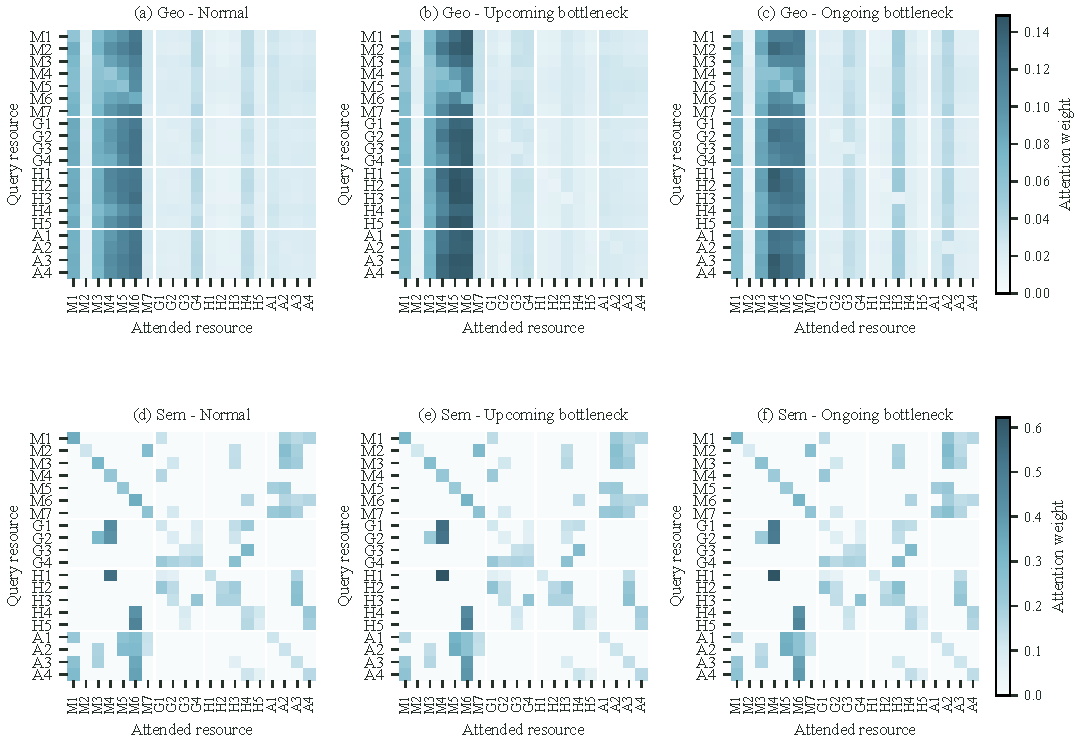
\includegraphics[width=0.92\textwidth]{figures/attention_heatmaps/fig02_resource_attention_states.pdf}
\caption{Absolute geographic (upper) and semantic (lower) resource attention under normal, upcoming, and ongoing conditions.}
\label{fig:attn-states}
\end{figure*}

\begin{figure*}[t]
\centering
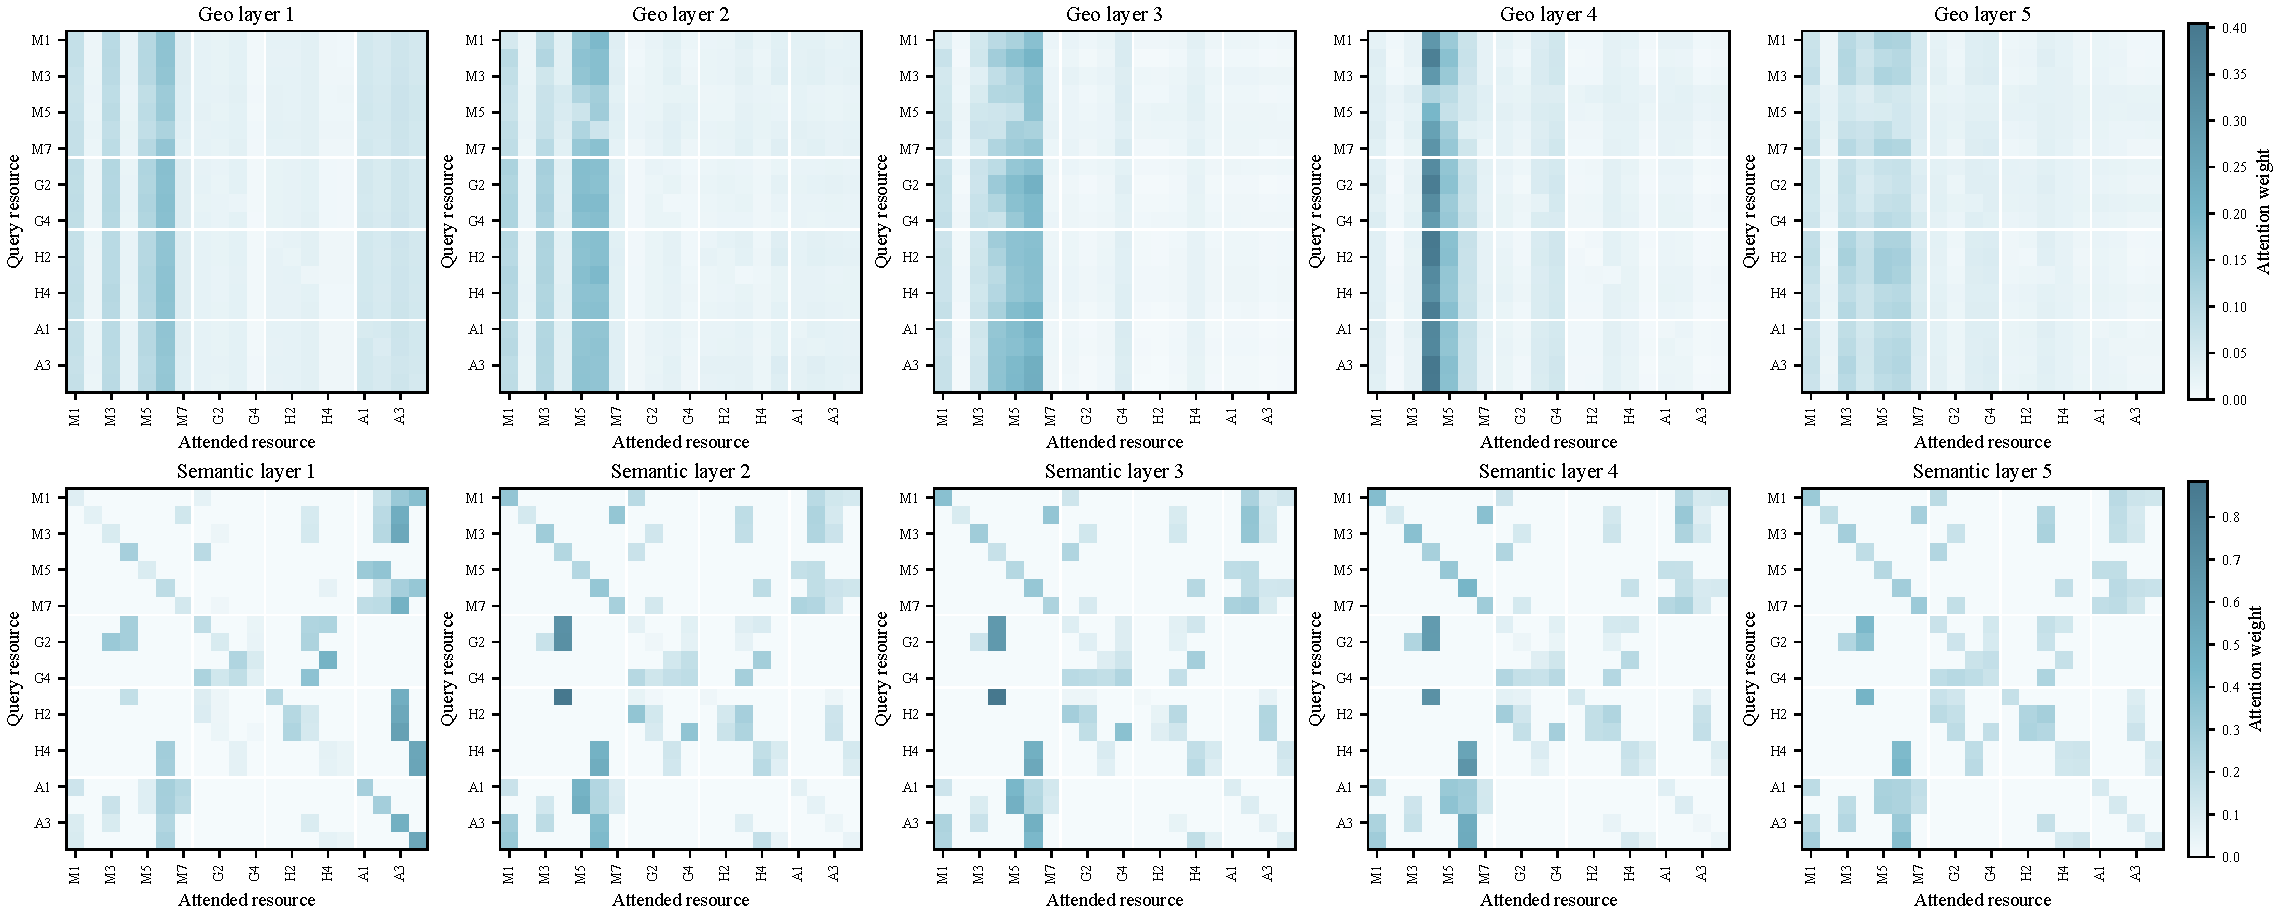
\includegraphics[width=0.94\textwidth]{figures/attention_heatmaps/fig05_layerwise_upcoming_attention.pdf}
\caption{Geographic (upper) and semantic (lower) attention across encoder layers 1--5 for upcoming samples.}
\label{fig:attn-layers-all}
\end{figure*}

\end{document}
